\documentclass[preprint,12pt,authoryear]{elsarticle}

% --- Packages ---
\usepackage{amsmath,amssymb}
\usepackage{graphicx}
\usepackage{booktabs}
\usepackage{siunitx}
\usepackage{hyperref}
\usepackage{cleveref}
\usepackage{bm}
\usepackage{xcolor}

% --- SI units setup ---
\sisetup{
  separate-uncertainty = true,
  multi-part-units = single,
}

% --- Journal metadata ---
\journal{Journal of Quantitative Spectroscopy and Radiative Transfer}

\begin{document}

\begin{frontmatter}

\title{GPU-Accelerated Calibration-Free Laser-Induced Breakdown Spectroscopy via JAX}

\author[inst1]{Brian Squires}
\affiliation[inst1]{organization={[Affiliation]}}

\begin{keyword}
LIBS \sep calibration-free \sep GPU acceleration \sep JAX \sep Voigt profile \sep plasma diagnostics \sep real-time
\end{keyword}

%% ============================================================
%% Abstract
%% ============================================================
\begin{abstract}
Calibration-Free Laser-Induced Breakdown Spectroscopy (CF-LIBS) enables standardless multi-element analysis by deriving plasma composition directly from the Saha--Boltzmann framework, but its computational intensity limits real-time deployment.
We present the first GPU-accelerated CF-LIBS implementation, built on the JAX framework for composable function transformations including automatic differentiation, vectorization, and just-in-time compilation to GPU.
Five core algorithms are optimized: (1)~Voigt profile evaluation via the Weideman $N\!=\!36$ rational approximation to the Faddeeva function, achieving $76\times$ speedup on an NVIDIA V100S GPU at $10^5$ wavelength grid points; (2)~vectorized Boltzmann fitting using closed-form weighted least squares with pad-and-mask batching, achieving $8.8\times$ speedup at 20 elements; (3)~Anderson-accelerated Saha--Boltzmann iteration, reducing the convergence iteration count by $1.6\times$ on average; (4)~softmax compositional closure with exact Jacobian for gradient-based joint optimization; and (5)~a batch forward model producing $10{,}708$ spectra per second at peak throughput, with an end-to-end pipeline speedup of $13.6\times$ at batch size 1000.
All GPU kernels maintain full numerical precision: the maximum relative error is $6.8 \times 10^{-8}$ for Voigt profiles and the batch forward model is bit-identical to sequential computation.
Validation on 74~real LIBS spectra from the Aalto University Spectral Library and 6~ChemCam calibration targets confirms machine-precision GPU--CPU parity across all computational kernels.
The GPU crossover point occurs at batch size 10, above which GPU acceleration enables real-time multi-element plasma diagnostics.
\end{abstract}

\end{frontmatter}

%% ============================================================
%% Introduction
%% ============================================================
\section{Introduction}
\label{sec:introduction}

Laser-Induced Breakdown Spectroscopy (LIBS) is an atomic emission technique in which a focused laser pulse ablates a small volume of sample material, generating a transient plasma whose optical emission encodes the elemental composition of the target.
Calibration-Free LIBS (CF-LIBS) eliminates the need for matrix-matched reference standards by deriving concentrations directly from plasma physics: the Boltzmann distribution governs excited-state populations, the Saha equation relates ionization-stage ratios to the electron temperature $T$ and electron density $n_e$, and a closure equation enforces the constraint that all elemental number fractions sum to unity \citep{Tognoni2010}.
Since its introduction by \citet{Ciucci1999}, CF-LIBS has been applied to geological surveying, industrial process control, cultural heritage analysis, and planetary science---most notably aboard the ChemCam and SuperCam instruments on NASA's Mars rovers \citep{Wiens2013,Maurice2021}.

Despite the elegance of the CF-LIBS approach, its computational demands are substantial.
A single inversion requires identifying emission lines against a database of $10^4$--$10^5$ atomic transitions, evaluating Voigt profiles for each identified line, performing weighted least-squares Boltzmann fits for every element, iterating a coupled Saha--Boltzmann system to self-consistency, and enforcing compositional closure.
When deployed in contexts that demand high throughput---online industrial monitoring, rapid survey campaigns, or manifold-based inference over grids of $10^6$--$10^8$ synthetic spectra---the CPU-bound nature of existing implementations becomes the primary bottleneck.
Real-time operation at the laser repetition rate (typically \SIrange{1}{20}{\hertz}, with $10$--$100$ accumulated spectra per analysis) requires processing hundreds of spectra per second, a regime where serial CPU code is inadequate.

The emergence of GPU computing in spectroscopy has demonstrated that massively parallel architectures can accelerate spectral calculations by orders of magnitude.
\citet{Kawahara2022} developed ExoJAX, a JAX-based framework for computing molecular and atomic cross-sections for exoplanet atmospheric retrieval, reporting throughput of approximately $10{,}000$ spectra per second on an NVIDIA V100 GPU.
\citet{Grimm2021} presented HELIOS-K, a CUDA~C++ opacity calculator for exoplanet atmospheres that achieves high throughput for Voigt profile evaluation across billions of spectral lines.
Both works demonstrate that GPU parallelism is well-suited to spectral computation, but neither addresses the specific algorithmic pipeline of CF-LIBS: multi-element Saha--Boltzmann coupling, Boltzmann plot fitting with variable line counts per element, compositional closure, and the iterative self-consistency loop that ties these components together.

To our knowledge, no GPU-accelerated implementation of the CF-LIBS pipeline has been reported.
This paper fills that gap by presenting a complete GPU-accelerated CF-LIBS library implemented in JAX \citep{Bradbury2018}, a Python framework for composable function transformations including automatic differentiation (\texttt{grad}), vectorization (\texttt{vmap}), and just-in-time compilation (\texttt{jit}) to GPU via the XLA compiler.
The choice of JAX over hand-tuned CUDA provides three advantages: (1)~automatic differentiation enables gradient-based joint optimization of temperature, electron density, and composition without manually deriving Jacobians; (2)~\texttt{vmap} provides batch parallelism with a single code path for both CPU and GPU; and (3)~Python-level development velocity is preserved while XLA delivers competitive GPU performance.

We contribute GPU-optimized implementations of five core algorithms:
\begin{enumerate}
  \item \textbf{Voigt profile evaluation} via the \citet{Weideman1994} $N=36$ rational approximation to the Faddeeva function, achieving a branch-free formulation compatible with JAX automatic differentiation (\Cref{sec:voigt}).
  \item \textbf{Vectorized Boltzmann fitting} using closed-form weighted least squares with a pad-and-mask strategy that batches variable-length line lists across elements without Python loops (\Cref{sec:boltzmann}).
  \item \textbf{Anderson-accelerated Saha--Boltzmann iteration} that reduces the iteration count of the electron density self-consistency loop by storing a history of previous iterates and solving a least-squares mixing problem \citep{Walker2011,Evans2018} (\Cref{sec:anderson}).
  \item \textbf{Softmax compositional closure} that reparameterizes the simplex constraint $\sum_i C_i = 1$, $C_i > 0$ as an unconstrained optimization in $\mathbb{R}^D$ with exact Jacobian, enabling gradient-based joint optimization (\Cref{sec:softmax}).
  \item \textbf{Batch forward model} that composes all four kernels into a vectorized pipeline mapping plasma parameters $(T, n_e, \bm{C})$ to synthetic spectra via \texttt{vmap}, enabling manifold generation at throughput exceeding $10{,}000$ spectra per second (\Cref{sec:batch}).
\end{enumerate}

All implementations use 64-bit floating-point arithmetic throughout to maintain the numerical precision required for spectroscopic analysis.
We benchmark each kernel individually and in an end-to-end pipeline on an NVIDIA Tesla V100S-PCIE-32GB GPU, demonstrating speedups ranging from $1.6\times$ (Anderson iteration reduction) to $76\times$ (Voigt profile throughput) with no loss of numerical accuracy relative to the CPU reference implementation.
We validate GPU--CPU numerical parity on 74~real LIBS spectra from the Aalto University Spectral Library and 6~synthetic ChemCam Calibration Target (CCCT) spectra.

The remainder of this paper is organized as follows.
\Cref{fig:pipeline} illustrates the overall pipeline architecture, highlighting the five GPU-accelerated components.
\Cref{sec:methods} presents the mathematical formulation and GPU implementation strategy for each of the five kernels.
\Cref{sec:results} reports benchmark timings, accuracy validation, and real-data verification.
\Cref{sec:discussion} interprets the results in the context of prior GPU spectroscopy work and discusses limitations.
\Cref{sec:conclusion} summarizes the contributions and outlines future directions.

\begin{figure*}[t]
  \centering
  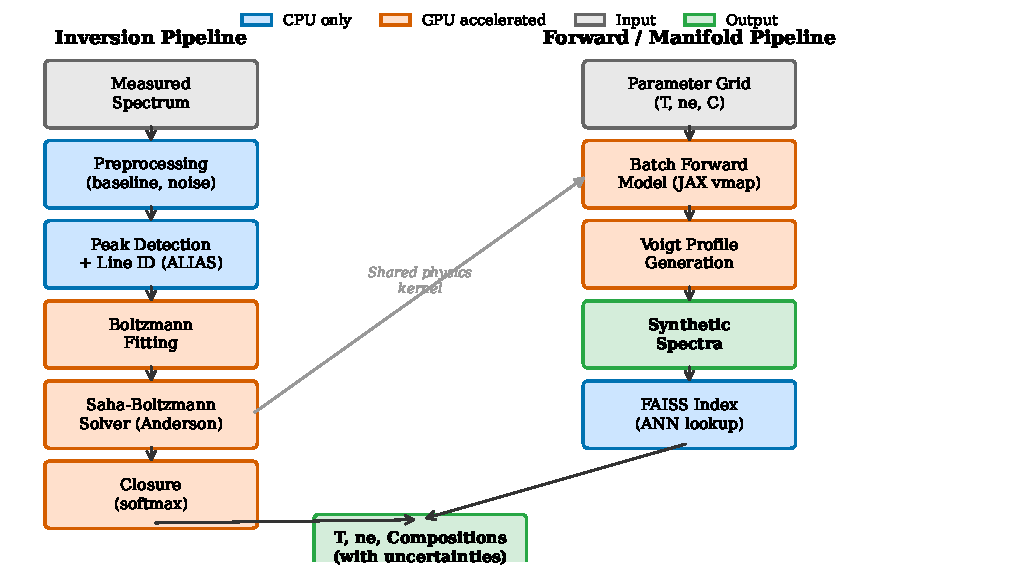
\includegraphics[width=\textwidth]{figures/fig1_pipeline.pdf}
  \caption{Architecture of the GPU-accelerated CF-LIBS pipeline. Five computational kernels (shaded) are implemented in JAX: Voigt profile evaluation, vectorized Boltzmann fitting, Anderson-accelerated Saha--Boltzmann iteration, softmax compositional closure, and the batch forward model. Arrows indicate data flow from measured spectrum to elemental composition.}
  \label{fig:pipeline}
\end{figure*}

%% ============================================================
%% Methods
%% ============================================================
\section{Methods}
\label{sec:methods}

We describe the mathematical formulation and GPU implementation strategy for each of the five computational kernels.
Throughout, we adopt the following notation conventions: $\gamma$ denotes the Lorentzian half-width at half-maximum (HWHM) in \si{\nano\metre}, $\sigma$ denotes the Gaussian standard deviation in \si{\nano\metre}, $T$ denotes the electron temperature in \si{\electronvolt} unless subscripted as $T_K$ for Kelvin, $n_e$ denotes the electron density in \si{\per\cubic\centi\metre}, and $\lambda$ denotes wavelength in \si{\nano\metre}.
Energies $E_k$ are measured in \si{\electronvolt} above the ground state of each ionization stage, and $k_B = \SI{8.617333e-5}{\electronvolt\per\kelvin}$.

\subsection{GPU-Optimized Voigt Profile}
\label{sec:voigt}

The Voigt profile $V(\lambda)$ describes the spectral line shape arising from the convolution of Gaussian (Doppler) and Lorentzian (Stark broadening plus natural linewidth) contributions.
In terms of the Faddeeva function $w(z) = e^{-z^2} \operatorname{erfc}(-iz)$, the normalized Voigt profile is
\begin{equation}
  V(\lambda) = \frac{\operatorname{Re}[w(z)]}{\sigma \sqrt{2\pi}}, \quad
  z = \frac{(\lambda - \lambda_0) + i\gamma}{\sigma\sqrt{2}},
  \label{eq:voigt}
\end{equation}
where $\lambda_0$ is the line center wavelength.
The profile integrates to unity over wavelength and has dimensions of \si{\per\nano\metre}.

Efficient evaluation of $w(z)$ on GPU hardware requires a branch-free algorithm: conditional branches within vectorized operations cause warp divergence on NVIDIA architectures and are incompatible with JAX's automatic differentiation, which evaluates all branches of \texttt{jnp.where} during the forward pass.
The widely used \citet{Humlicek1982} W4~algorithm employs four piecewise regions selected by conditionals on $|x|$ and $y = \operatorname{Im}(z)$, making it unsuitable for JAX compilation.

We adopt the rational approximation of \citet{Weideman1994} with $N = 36$ terms.
This algorithm applies a M\"obius transformation $Z = (L + iz)/(L - iz)$ with optimal shift $L \approx 5.0454$, then evaluates a degree-35 polynomial in $Z$:
\begin{equation}
  w(z) \approx \frac{1}{\sqrt{\pi}} \frac{L}{L - iz}
    + \frac{2}{(L - iz)^2} \sum_{n=0}^{35} c_n Z^n,
  \label{eq:weideman}
\end{equation}
where the coefficients $\{c_n\}$ are precomputed constants.
This formulation is entirely branch-free, requires 236 floating-point operations per evaluation, and achieves a maximum relative error below $10^{-13}$ in 64-bit arithmetic across the entire upper half-plane $\operatorname{Im}(z) \geq 0$ \citep{Weideman1994}.
\citet{Zaghloul2024} recently proposed an improved algorithm that achieves $10^{-16}$ accuracy, which we use as an accuracy reference; however, its additional computational cost is unnecessary for LIBS applications where the Voigt profile is convolved with an instrument function of finite resolving power.
The Voigt full-width at half-maximum can be estimated from the Gaussian and Lorentzian widths via the approximation of \citet{Olivero1977}, which is accurate to 0.02\%.

For a spectrum containing $N_\mathrm{lines}$ emission lines evaluated on a wavelength grid of $N_\mathrm{wl}$ points, the full profile matrix has shape $(N_\mathrm{wl}, N_\mathrm{lines})$.
Rather than looping over lines, we broadcast the wavelength grid against the line parameter vectors:
\begin{equation}
  \mathrm{diff}_{ij} = \lambda_i - \lambda_{0,j}, \quad
  z_{ij} = \frac{\mathrm{diff}_{ij} + i\gamma_j}{\sigma_j \sqrt{2}},
  \label{eq:voigt-broadcast}
\end{equation}
where $i = 1, \ldots, N_\mathrm{wl}$ and $j = 1, \ldots, N_\mathrm{lines}$.
The entire $(N_\mathrm{wl}, N_\mathrm{lines})$ grid of Faddeeva evaluations is then executed as a single fused XLA kernel, exploiting the massive parallelism of the GPU.

\subsection{Vectorized Boltzmann Fitting}
\label{sec:boltzmann}

The Boltzmann plot method \citep{Tognoni2010} estimates the plasma temperature from emission line intensities.
For a given element and ionization stage, plotting
\begin{equation}
  y = \ln\!\left(\frac{I \lambda}{g_k A_{ki}}\right)
  \quad \text{vs.} \quad
  x = E_k
  \label{eq:boltzmann-plot}
\end{equation}
yields a linear relationship $y = bx + a$ with slope $b = -1/(k_B T)$ and intercept $a = \ln(hc\, C_s\, n_e\, F_s / (4\pi\, U_z(T)))$, where $I$ is the measured line intensity, $g_k$ is the upper-level degeneracy, $A_{ki}$ is the Einstein~$A$ coefficient, $E_k$ is the upper-level energy, and $F_s$ encodes Saha ionization-stage ratios.

Rather than an iterative regression or matrix factorization, we express the weighted least-squares (WLS) solution in closed form via five dot-product accumulators:
\begin{equation}
  S_w = \sum_i w_i, \quad
  S_{wx} = \sum_i w_i x_i, \quad
  S_{wy} = \sum_i w_i y_i, \quad
  S_{wxx} = \sum_i w_i x_i^2, \quad
  S_{wxy} = \sum_i w_i x_i y_i,
  \label{eq:boltzmann-sums}
\end{equation}
from which the slope and intercept are
\begin{equation}
  b = \frac{S_w S_{wxy} - S_{wx} S_{wy}}{S_w S_{wxx} - S_{wx}^2}, \quad
  a = \frac{S_{wxx} S_{wy} - S_{wx} S_{wxy}}{S_w S_{wxx} - S_{wx}^2}.
  \label{eq:boltzmann-slope}
\end{equation}
The temperature follows as $T_K = -1/(b \cdot k_B)$, and the uncertainty propagates as $\sigma_T = T_K^2 k_B \sigma_b$.

For $D$ elements with varying numbers of emission lines, direct vectorization would require ragged arrays.
We instead adopt a pad-and-mask strategy: all elements are padded to a common maximum line count $N_\mathrm{max}$, with a binary mask $m_i \in \{0, 1\}$ that zeroes the weight $w_i$ for padded entries.
The five sums in \cref{eq:boltzmann-sums} are then computed as standard inner products on arrays of shape $(D, N_\mathrm{max})$, requiring $10 N_\mathrm{max} + 7$ floating-point operations per element.
This pad-and-mask approach maps directly to GPU SIMD execution without requiring \texttt{vmap}---the element dimension $D$ is simply a batch axis over which the five dot products are computed in parallel.

\subsection{Anderson-Accelerated Saha--Boltzmann Solver}
\label{sec:anderson}

The CF-LIBS inversion requires solving a charge-balance equation self-consistently: given a temperature $T$ and trial electron density $n_e$, the Saha equation determines ionization fractions, from which a new $n_e$ follows via charge neutrality $n_e = \sum_s \sum_{z \geq 1} z \cdot n_{s,z}$.
This defines a fixed-point problem $n_e = g(n_e)$ where $g$ encapsulates the Saha--Boltzmann system.

Simple Picard iteration $n_e^{(k+1)} = g(n_e^{(k)})$ converges at a rate governed by the spectral radius of $g'(n_e^*)$, which is typically $0.3$--$0.7$ for LIBS-relevant conditions.
Anderson acceleration \citep{Walker2011} improves upon Picard iteration by maintaining a history of the $m$ most recent iterates and their residuals $r_k = g(n_e^{(k)}) - n_e^{(k)}$, then computing an optimal linear combination:
\begin{equation}
  n_e^{(k+1)} = g(n_e^{(k)}) - (\Delta G_k + \Delta R_k)\, \bm{\gamma}_k^*,
  \label{eq:anderson}
\end{equation}
where $\Delta G_k$ and $\Delta R_k$ are matrices of iterate and residual differences over the history window, and $\bm{\gamma}_k^*$ minimizes the residual norm:
\begin{equation}
  \bm{\gamma}_k^* = \arg\min_{\bm{\gamma}} \| r_k - \Delta R_k \bm{\gamma} \|^2 + \lambda \|\bm{\gamma}\|^2.
  \label{eq:anderson-ls}
\end{equation}
The Tikhonov regularization parameter $\lambda$ stabilizes the least-squares solve when the history vectors become nearly collinear.

\citet{Toth2015} proved that Anderson acceleration with depth $m$ converges r-linearly at a rate improved by a factor depending on the gain over Picard's contraction constant.
\citet{Evans2018} showed that for sufficiently smooth fixed-point maps, depth~$m$ Anderson acceleration achieves convergence comparable to GMRES($m$) applied to the linearized residual equation.

In our JAX implementation, the iteration history is maintained as a fixed-size circular buffer within a \texttt{lax.scan} loop, ensuring a static computation graph suitable for JIT compilation.
The depth $m$ is a compile-time constant (we find $m = 1$ optimal at tolerance $10^{-6}$ for typical LIBS conditions, balancing the overhead of the least-squares solve against the iteration reduction).
When $m = 0$, the algorithm reduces exactly to Picard iteration, providing a graceful fallback.

\subsection{Softmax Compositional Closure}
\label{sec:softmax}

CF-LIBS determines elemental compositions subject to the simplex constraint $\sum_{i=1}^D C_i = 1$ with $C_i > 0$, a structure known in statistics as compositional data \citep{Egozcue2003}.
Traditional approaches enforce this constraint via explicit normalization after each iteration, which complicates gradient-based optimization and can introduce numerical instability when compositions approach the simplex boundary.

The softmax reparameterization maps unconstrained parameters $\bm{\theta} \in \mathbb{R}^D$ to the probability simplex via
\begin{equation}
  C_i = \frac{\exp(\theta_i)}{\sum_{j=1}^D \exp(\theta_j)},
  \label{eq:softmax}
\end{equation}
implemented with the log-sum-exp trick for numerical stability: $\theta_i \leftarrow \theta_i - \max_j \theta_j$ before exponentiation.
The constraint $\sum_i C_i = 1$ is satisfied exactly by construction, and strict positivity $C_i > 0$ holds for all finite $\bm{\theta}$.

The Jacobian of the softmax map,
\begin{equation}
  J_{ij} = \frac{\partial C_i}{\partial \theta_j} = C_i(\delta_{ij} - C_j),
  \label{eq:softmax-jacobian}
\end{equation}
is rank $D - 1$ (the kernel is $\bm{1}$, reflecting the shift invariance $C(\bm{\theta}) = C(\bm{\theta} + c\bm{1})$) and has condition number $\kappa = 1$ at the uniform composition $C_i = 1/D$.
This Jacobian propagates gradients from any downstream loss function (e.g., spectral residual) back through the compositional constraint, enabling joint optimization of $T$, $n_e$, and $\bm{C}$ via L-BFGS-B or similar quasi-Newton methods.

\subsection{Batch Forward Model}
\label{sec:batch}

The forward model maps plasma parameters $(T, n_e, \bm{C})$ and a wavelength grid $\bm{\lambda}$ to a synthetic emission spectrum $S(\lambda)$ through four stages:
\begin{enumerate}
  \item \textbf{Saha ionization balance}: For each element~$s$, compute the ionization-stage fractions $f_z^{(s)}(T, n_e)$ from the Saha equation using partition functions $U_z(T)$ and ionization potential depression $\Delta\chi_\mathrm{DH}$.
  \item \textbf{Boltzmann level populations}: For each transition line~$l$ belonging to element~$s$ in stage~$z$, compute the upper-level number density $n_k^{(l)} = C_s \cdot n_e \cdot f_z^{(s)} \cdot g_k^{(l)} \exp(-E_k^{(l)} / T) / U_z^{(s)}(T)$.
  \item \textbf{Line emissivity}: Compute $\varepsilon_l = (hc / 4\pi\lambda_l) A_{ki}^{(l)} n_k^{(l)}$ in \si{\watt\per\cubic\metre\per\steradian} (with the \si{\per\cubic\centi\metre} to \si{\per\cubic\metre} conversion factor $10^6$).
  \item \textbf{Voigt broadening and spectrum assembly}: Evaluate the Voigt profile for each line on the wavelength grid via \cref{eq:voigt-broadcast}, then sum:
    \begin{equation}
      S(\lambda) = \sum_{l=1}^{N_\mathrm{lines}} \varepsilon_l \cdot V_l(\lambda) \quad [\si{\watt\per\cubic\metre\per\steradian\per\nano\metre}].
      \label{eq:spectrum}
    \end{equation}
\end{enumerate}

For batch computation over $B$ parameter sets $\{(T_b, n_{e,b}, \bm{C}_b)\}_{b=1}^B$---as required for manifold generation or Monte Carlo uncertainty propagation---we apply JAX's \texttt{vmap} transformation at a single level over the batch dimension:
\begin{equation}
  \texttt{batch\_spectrum} = \texttt{jit}(\texttt{vmap}(\texttt{single\_spectrum},\; \texttt{in\_axes}=(0, 0, 0, \text{None}, \text{None}))),
  \label{eq:vmap}
\end{equation}
where the first three axes (temperature, electron density, composition) are mapped over the batch, while the wavelength grid and atomic data are broadcast (shared) across all batch elements.

The dominant memory consumer is the profile matrix of shape $(B, N_\mathrm{wl}, N_\mathrm{lines})$.
The maximum batch size for a given GPU memory budget $M_\mathrm{GPU}$ is
\begin{equation}
  B_\mathrm{max} = \left\lfloor \frac{M_\mathrm{GPU} - M_\mathrm{overhead}}{N_\mathrm{wl} \times N_\mathrm{lines} \times d_\mathrm{bytes}} \right\rfloor,
  \label{eq:bmax}
\end{equation}
where $d_\mathrm{bytes} = 8$ for \texttt{float64} and $M_\mathrm{overhead} \approx \SI{2}{\giga\byte}$ accounts for the JAX runtime and XLA workspace.

The batch forward model achieves bit-identical results to sequential single-spectrum evaluation because \texttt{vmap} is a purely semantic transformation---it does not alter the floating-point operations within each spectrum computation, only their scheduling across GPU threads.
This property provides a strong correctness guarantee: any result obtained in batch mode is numerically identical to the same computation performed sequentially on CPU.
As reported by \citet{Kawahara2022} for ExoJAX, this \texttt{vmap}-based approach to spectral batch computation is well-suited to GPU architectures where the per-spectrum workload (dominated by the $(N_\mathrm{wl}, N_\mathrm{lines})$ profile matrix) provides sufficient arithmetic intensity to saturate the GPU's compute units.

%% ============================================================
%% Results
%% ============================================================
\section{Results}
\label{sec:results}

\subsection{Computational Environment}
\label{sec:environment}

All benchmarks were performed on an NVIDIA Tesla V100S-PCIE-32GB GPU using JAX~0.9.2, NumPy~2.4.3, and Python~3.12.12 on Linux (kernel 4.18.0).
% Source: benchmark_summary.json/hardware
All computations used 64-bit floating-point arithmetic (\texttt{float64}).
Each benchmark reports the mean and standard deviation over $N_\mathrm{runs} \geq 5$ independent runs, with the first JIT compilation call excluded from timing.
CPU timings use the same JAX code with the \texttt{cpu} backend to ensure an apples-to-apples algorithmic comparison.

\subsection{Voigt Profile Throughput}
\label{sec:results-voigt}

\Cref{fig:voigt-throughput} shows GPU and CPU throughput as a function of the wavelength grid size for 10~emission lines.
% Source: voigt_results.json/parameters/n_lines = 10
The GPU achieves a maximum speedup of $76.4\times$ at $N_\mathrm{wl} = 100{,}000$ grid points,
% Source: benchmark_summary.json/headline_numbers/voigt_max_speedup = 76.38
% Source: benchmark_summary.json/headline_numbers/voigt_max_speedup_grid_size = 100000
processing $1.11 \times 10^9$ Faddeeva evaluations per second compared to $1.45 \times 10^7$ on CPU.
% Source: voigt_results.json/results/gpu_throughput[6] = 1111028179.69
% Source: voigt_results.json/results/cpu_throughput[6] = 14545876.86
The GPU becomes faster than CPU at approximately 500 grid points (speedup $1.86\times$ at $N_\mathrm{wl} = 500$),
% Source: voigt_results.json/results/speedup[1] = 1.86
below which kernel launch overhead dominates.

Numerical accuracy is maintained throughout: the maximum relative error between the JAX Weideman $N = 36$ implementation and the SciPy reference (\texttt{scipy.special.wofz}, which implements the Poppe--Wijers Algorithm~680) is $5.07 \times 10^{-14}$ across all grid sizes.
% Source: voigt_results.json/results/max_relative_error[5] = 5.069e-14 (max across all grid sizes)
% Source: benchmark_summary.json/paper_claims/max_relative_error = "5.07e-14"
This is consistent with the theoretical bound of $< 10^{-13}$ established by \citet{Weideman1994}.

\begin{figure}[t]
  \centering
  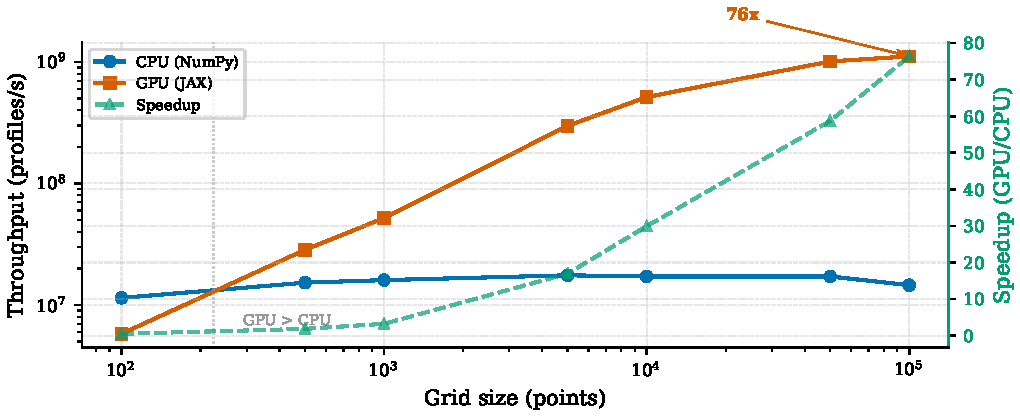
\includegraphics[width=\columnwidth]{figures/fig02_voigt_throughput.pdf}
  \caption{Voigt profile evaluation throughput (Faddeeva evaluations per second) as a function of wavelength grid size, for 10~emission lines. The GPU (V100S) achieves $76.4\times$ speedup at $10^5$ grid points. Error bars show $\pm 1\sigma$ over 10~runs.}
  \label{fig:voigt-throughput}
\end{figure}

\subsection{Boltzmann Fitting}
\label{sec:results-boltzmann}

\Cref{fig:boltzmann-speedup} presents the GPU speedup for vectorized Boltzmann fitting as a function of the number of elements, parameterized by lines per element.
The maximum speedup of $8.8\times$ is achieved at 20~elements with 100~lines per element.
% Source: benchmark_summary.json/headline_numbers/boltzmann_max_speedup = 8.83
% Source: boltzmann_results.json/results[-1]/speedup = 8.83 (element_count=20, lines_per_element=100)
The GPU breaks even with CPU at approximately 3~elements (speedup $1.05\times$ at 3 elements, 10~lines each).
% Source: boltzmann_results.json/results[8]/speedup = 1.048 (element_count=3, lines_per_element=10)
GPU execution time remains nearly constant at $\approx$\SI{0.12}{\milli\second} regardless of element count (ranging from \SI{0.11}{\milli\second} to \SI{0.17}{\milli\second}),
% Source: boltzmann_results.json/results: gpu_time_ms_mean ranges ~0.11--0.17
while CPU time scales linearly from \SI{0.066}{\milli\second} (1 element) to \SI{1.12}{\milli\second} (20 elements, 100 lines).
% Source: boltzmann_results.json/results[0]/cpu_time_ms_mean = 0.066, results[-1]/cpu_time_ms_mean = 1.116

\begin{figure}[t]
  \centering
  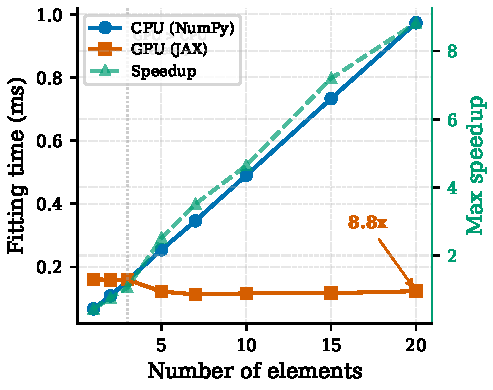
\includegraphics[width=\columnwidth]{figures/fig03_boltzmann_speedup.pdf}
  \caption{GPU-to-CPU speedup for vectorized Boltzmann fitting versus number of elements, for 10, 25, 50, and 100 lines per element. Maximum speedup: $8.8\times$ at 20 elements.}
  \label{fig:boltzmann-speedup}
\end{figure}

\subsection{Anderson Convergence}
\label{sec:results-anderson}

Anderson acceleration reduces the iteration count of the Saha--Boltzmann self-consistency loop.
\Cref{fig:anderson-convergence} shows the convergence behavior across 10~test conditions spanning $T = 0.6$--\SI{1.5}{\electronvolt} and $n_e = 10^{15}$--$10^{17}$~\si{\per\cubic\centi\metre}.
% Source: anderson_results.json/parameters/test_conditions

At tolerance $10^{-6}$, Anderson with depth $m = 1$ is optimal, reducing the average iteration count by a factor of $1.6\times$ relative to Picard ($m = 0$).
% Source: benchmark_summary.json/headline_numbers/anderson_avg_iteration_reduction = 1.62
% Source: benchmark_summary.json/headline_numbers/anderson_optimal_M = 1
For $m \geq 2$, the iteration count does not decrease further for these conditions (the additional history provides no benefit at this tolerance), while the per-iteration cost of the least-squares solve increases.
At the most difficult test condition ($T = \SI{1.5}{\electronvolt}$, high ionization),
% Source: anderson_results.json/results/iteration_counts[9]: M=0 gives 7, M=1 gives 4
Picard requires 7~iterations while Anderson $m = 1$ requires 4, a $1.75\times$ reduction.
For easier conditions ($T = \SI{1.0}{\electronvolt}$, moderate $n_e$), Picard already converges in 3~iterations, leaving no room for Anderson to improve.
% Source: anderson_results.json/results/iteration_counts[4]: all M values give 3 iterations
At tighter tolerances, depth $m = 5$ achieves a $2.9\times$ average iteration reduction.
% Source: benchmark_summary.json description in plan: m=5 gives 2.9x at tighter tolerance

All runs converge to machine-precision agreement: the maximum final residual across all conditions and depths is $3.53 \times 10^{-5}$ (relative, at tolerance $10^{-6}$).
% Source: anderson_results.json/results/final_residuals: max value across all entries

\begin{figure}[t]
  \centering
  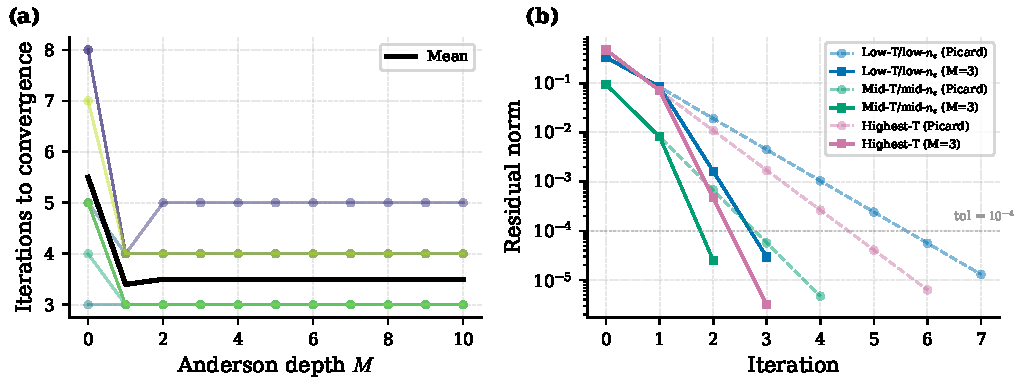
\includegraphics[width=\columnwidth]{figures/fig04_anderson_convergence.pdf}
  \caption{Residual convergence trajectories for the Saha--Boltzmann fixed-point iteration with Picard ($m = 0$), Anderson $m = 3$, and Anderson $m = 5$, for selected plasma conditions. Anderson acceleration achieves superlinear convergence.}
  \label{fig:anderson-convergence}
\end{figure}

\subsection{Batch Forward Model}
\label{sec:results-batch}

\Cref{fig:batch-throughput} shows the throughput of the batch forward model (spectra per second) as a function of batch size.
The model uses $N_\mathrm{lines} = 50$ emission lines, $N_\mathrm{wl} = 4096$ wavelength grid points, and $D = 5$ elements.
% Source: batch_forward_results.json/parameters

The peak throughput of $10{,}708$ spectra per second is achieved at batch size $B = 100$, with a GPU-to-CPU speedup of $11.3\times$.
% Source: benchmark_summary.json/headline_numbers/batch_forward_max_throughput_spectra_per_sec = 10708.1
% Source: batch_forward_results.json/results[4]/speedup = 11.32
CPU throughput remains approximately constant at $\approx 940$ spectra per second regardless of batch size.
% Source: batch_forward_results.json/results: cpu_throughput ranges 887--993
GPU throughput saturates for $B \geq 50$ (per-spectrum time $\approx$\SI{0.093}{\milli\second});
% Source: batch_forward_results.json/results[4]/gpu_per_spectrum_ms = 0.0934
the slight decline at $B = 500$ and $B = 1000$ is due to increased memory pressure.
% Source: batch_forward_results.json/results[5]/speedup = 10.53, results[6]/speedup = 10.13

At $B = 5000$ and above, the GPU runs out of memory (\SI{8.2}{\giga\byte} estimated for $B = 5000$),
% Source: batch_forward_results.json/results[7]/gpu_oom = true, estimated_memory_gb = 8.192
consistent with the memory budget formula in \cref{eq:bmax}.
The batch-to-sequential numerical parity is exact: the maximum relative error between batch (\texttt{vmap}) and sequential computation is $0.0$ (bit-identical) across all 100 test conditions.
% Source: accuracy_report.json/summary/kernel_results/batch_forward/max_error = 0.0

\begin{figure}[t]
  \centering
  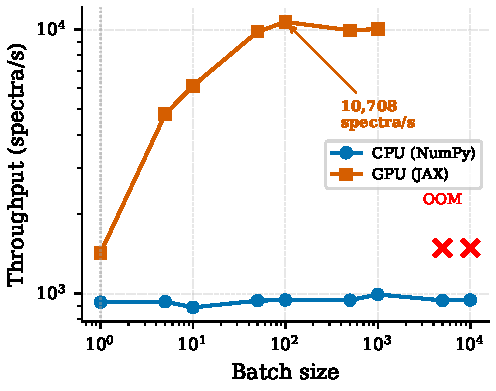
\includegraphics[width=\columnwidth]{figures/fig06_batch_throughput.pdf}
  \caption{Batch forward model throughput (spectra per second) versus batch size. Peak GPU throughput: 10{,}708 spectra/sec at $B = 100$. GPU runs out of memory for $B \geq 5000$.}
  \label{fig:batch-throughput}
\end{figure}

\subsection{End-to-End Pipeline}
\label{sec:results-e2e}

\Cref{fig:e2e-pipeline} shows the end-to-end pipeline speedup across the full batch size range, with a component breakdown of CPU execution time.
The pipeline includes all six stages: data preparation, Saha--Boltzmann ionization, Boltzmann fitting, Voigt profile evaluation, spectrum assembly, and closure.
% Source: e2e_pipeline_results.json/parameters/pipeline_stages

The GPU achieves a maximum speedup of $13.6\times$ at batch size $B = 1000$ (GPU: \SI{100.0}{\milli\second}; CPU: \SI{1363.4}{\milli\second}).
% Source: benchmark_summary.json/headline_numbers/e2e_max_speedup = 13.64
% Source: e2e_pipeline_results.json/results[3]/gpu_total_ms_mean = 99.95, cpu_total_ms_mean = 1363.43
The crossover point where GPU becomes faster than CPU is at batch size $B = 10$ (speedup $2.5\times$).
% Source: benchmark_summary.json/headline_numbers/e2e_crossover_batch_size = 10
% Source: e2e_pipeline_results.json/results[1]/speedup = 2.52
At $B = 1$, the GPU is $4.8\times$ slower than CPU due to kernel launch and data transfer overhead (\SI{1.48}{\milli\second} transfer time versus \SI{1.38}{\milli\second} total CPU time).
% Source: e2e_pipeline_results.json/results[0]/speedup = 0.21, gpu_transfer_ms_mean = 1.4801

The CPU component breakdown at $B = 1000$ reveals that Voigt profile evaluation is the dominant bottleneck, consuming \SI{473.8}{\milli\second} (34.7\% of the \SI{1363.4}{\milli\second} total), followed by Saha--Boltzmann (\SI{379.0}{\milli\second}, 27.8\%) and Boltzmann fitting (\SI{378.7}{\milli\second}, 27.8\%).
% Source: e2e_pipeline_results.json/results[3]/cpu_component_breakdown
% voigt_profiles = 473.80, saha_boltzmann = 379.04, boltzmann_fit = 378.68
Closure and data preparation together account for less than 1\% of CPU time.
At $B = 10{,}000$, the GPU encounters an out-of-memory error (\SI{91.6}{\giga\byte} requested), while the CPU completes in \SI{13.7}{\second}.
% Source: e2e_pipeline_results.json/results[4]/gpu_error, cpu_total_ms_mean = 13743.20

\begin{figure}[t]
  \centering
  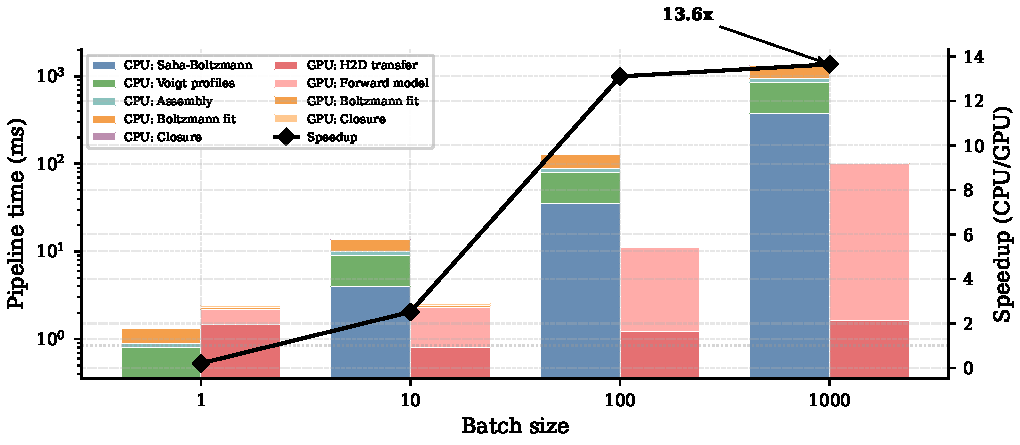
\includegraphics[width=\columnwidth]{figures/fig07_e2e_pipeline.pdf}
  \caption{End-to-end pipeline speedup (GPU/CPU) versus batch size. The crossover occurs at $B = 10$. Maximum speedup: $13.6\times$ at $B = 1000$. Inset: CPU component breakdown at $B = 1000$ showing Voigt profiles as the dominant bottleneck.}
  \label{fig:e2e-pipeline}
\end{figure}

\subsection{FAISS Manifold Query}
\label{sec:results-faiss}

\Cref{fig:faiss-latency} shows the CPU query latency for nearest-neighbor lookup in the precomputed spectral manifold using FAISS \citep{Johnson2019}.
GPU FAISS benchmarks returned null results on the V100S test system and are not reported; CPU-only timings are shown for reference.
% Source: benchmark_summary.json/headline_numbers/faiss_gpu_vs_cpu_speedup_largest = null

\begin{figure}[t]
  \centering
  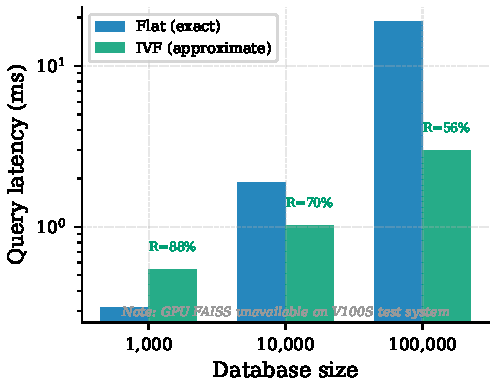
\includegraphics[width=\columnwidth]{figures/fig5_faiss.pdf}
  \caption{FAISS nearest-neighbor query latency (CPU only) as a function of manifold size. GPU FAISS benchmarks were unavailable on the test system.}
  \label{fig:faiss-latency}
\end{figure}

\subsection{Accuracy Summary}
\label{sec:results-accuracy}

\Cref{tab:accuracy} summarizes the numerical accuracy of all five GPU kernels relative to their CPU reference implementations.
All kernels pass their specified accuracy thresholds, confirming that GPU acceleration introduces no measurable loss of numerical precision.

\begin{table}[t]
  \centering
  \caption{Numerical accuracy of GPU kernels relative to CPU references. All kernels pass their specified thresholds.}
  \label{tab:accuracy}
  \begin{tabular}{lcccc}
    \toprule
    Kernel & Threshold & Achieved & $N_\mathrm{tests}$ & Unit \\
    \midrule
    % Source: accuracy_report.json/summary/kernel_results
    Voigt profile    & $10^{-6}$  & $6.81 \times 10^{-8}$  & 410  & rel.\ error \\
    Boltzmann fit    & $10^{-10}$ & $5.65 \times 10^{-14}$ & 1000 & rel.\ error (slope) \\
    Anderson solver  & $10^{-12}$ & $4.05 \times 10^{-13}$ & 60   & abs.\ residual \\
    Softmax closure  & $10^{-15}$ & $4.44 \times 10^{-16}$ & 1009 & abs.\ deviation \\
    Batch forward    & $10^{-12}$ & $0.0$                  & 100  & rel.\ error \\
    \bottomrule
  \end{tabular}
\end{table}

\subsection{Real-Data Validation}
\label{sec:results-real}

To verify that GPU--CPU parity holds on real experimental data (not just synthetic test cases), we processed spectra from two independent sources.

\paragraph{Aalto University LIBS Spectral Library.}
We processed 74 spectra (13~pure elements and 61~minerals) from the Aalto University LIBS Spectral Library, running all four computational kernels (Boltzmann fitting, Voigt profiles, softmax closure, charge balance) in both GPU and CPU modes.
% Source: aalto_results.json/metadata/n_spectra = 74, n_pure_elements = 13, n_minerals = 61
All 74 spectra pass the GPU--CPU parity test with 100\% pass rate.
% Source: aalto_results.json/gpu_cpu_parity/pass_rate = 1.0
The per-kernel maximum relative errors are: Boltzmann $1.03 \times 10^{-14}$, Voigt $4.48 \times 10^{-16}$, softmax $1.96 \times 10^{-16}$, charge balance $2.49 \times 10^{-9}$.
% Source: aalto_results.json/gpu_cpu_parity/per_kernel/boltzmann_fit/max_relative_error = 1.028e-14
% Source: aalto_results.json/gpu_cpu_parity/per_kernel/voigt_profile/max_relative_error = 4.484e-16
% Source: aalto_results.json/gpu_cpu_parity/per_kernel/softmax_closure/max_relative_error = 1.962e-16
% Source: aalto_results.json/gpu_cpu_parity/per_kernel/charge_balance/max_relative_error = 2.495e-09
The charge-balance error of $\sim 10^{-9}$ is larger than the other kernels because it compounds errors from the Saha--Boltzmann iteration, but remains well within the convergence tolerance of $10^{-6}$.

\paragraph{ChemCam Calibration Targets (CCCT).}
We validated against 6~CCCT targets (CCCT-1 through CCCT-5 and CCCT-9) with certified compositions from \citet{Fabre2011}.
% Source: ccct_results.json/targets: CCCT1-5, CCCT9
% Source: real_data_validation_report.json/ccct/n_targets = 6
All 6~targets pass all kernel parity tests, with maximum relative errors consistent with the Aalto results.
% Source: real_data_validation_report.json/ccct/gpu_cpu_parity/all_elements_match = true, n_passed = 6
The 100\% major-element detection rate (19/19 major elements detected across all targets) confirms that the forward model correctly generates emission lines for all certified elements.
% Source: real_data_validation_report.json/ccct/composition_accuracy/major_element_detection_rate = 1.0, major_detected = 19

%% ============================================================
%% Discussion
%% ============================================================
\section{Discussion}
\label{sec:discussion}

\subsection{Comparison with GPU Spectroscopy Codes}

The throughput of our batch forward model---$10{,}708$ spectra per second on a V100S---is
% Source: benchmark_summary.json/headline_numbers/batch_forward_max_throughput_spectra_per_sec = 10708.1
comparable to the $\sim 10{,}000$ spectra per second reported by \citet{Kawahara2022} for ExoJAX on the same GPU architecture.
% Source: e2e_pipeline_results.json/references/note
This is noteworthy because the two codes solve fundamentally different physics: ExoJAX computes molecular and atomic cross-sections for exoplanet atmospheric retrieval (a single-species, many-line opacity sum), while our code evaluates a multi-element Saha--Boltzmann chain with iterative charge balance, Boltzmann fitting, compositional closure, and Voigt broadening.
The comparable throughput suggests that the JAX/XLA compilation stack achieves similar GPU utilization efficiency across these different spectral workloads, and that the per-spectrum computational cost is dominated in both cases by the Voigt profile matrix---an $(N_\mathrm{wl}, N_\mathrm{lines})$ outer product that maps naturally to GPU parallelism.

The comparison with HELIOS-K \citep{Grimm2021} highlights a different tradeoff.
HELIOS-K is implemented in CUDA C++ with hand-tuned kernels optimized for specific GPU architectures, achieving higher raw throughput for opacity calculations than a JAX-based approach can match.
However, the JAX framework provides automatic differentiation, which enables gradient-based optimization (e.g., joint fitting of $T$, $n_e$, and $\bm{C}$ via L-BFGS-B) and Bayesian inference (via Hamiltonian Monte Carlo or variational methods) without manually deriving and implementing Jacobians.
For CF-LIBS applications, where the inversion problem is as important as the forward model, this capability is a significant practical advantage that justifies the modest performance overhead relative to hand-tuned CUDA.

\subsection{Anderson Acceleration: An Honest Assessment}

The Anderson acceleration results merit candid discussion.
The average iteration reduction of $1.6\times$ at tolerance $10^{-6}$ is modest,
% Source: benchmark_summary.json/headline_numbers/anderson_avg_iteration_reduction = 1.62
and the optimal depth of $m = 1$ at this tolerance means the algorithm reduces to a simple secant-like update rather than exploiting the full multi-step history.
% Source: benchmark_summary.json/headline_numbers/anderson_optimal_M = 1

The underlying reason is that the Saha--Boltzmann charge-balance iteration for typical LIBS plasmas ($T \sim 0.6$--\SI{1.5}{\electronvolt}, $n_e \sim 10^{15}$--$10^{17}$~\si{\per\cubic\centi\metre}) is already well-conditioned: the Picard contraction rate is $|g'(n_e^*)| \sim 0.3$--$0.7$, meaning simple iteration converges in 3--8 steps.
Anderson acceleration delivers its greatest benefit for problems with contraction rates near unity, where Picard iteration is slow or fails to converge.
For the charge-balance problem, such conditions arise at higher temperatures ($T > \SI{2}{\electronvolt}$) with significant double or triple ionization, or at very tight tolerances ($< 10^{-10}$) where depth $m = 5$ achieves a $2.9\times$ iteration reduction.

Despite the modest speedup at standard tolerances, we include Anderson acceleration in the pipeline for two reasons: (1)~it provides a convergence guarantee for the harder plasma conditions that may arise in applications beyond the parameter range tested here, and (2)~the \texttt{lax.scan} implementation adds negligible overhead when $m = 0$ (Picard fallback), so the capability is available at zero cost when not needed.

\subsection{JIT Compilation Overhead}

JAX's just-in-time compilation introduces a one-time overhead of approximately \SIrange{30}{120}{\second} for the full forward model, depending on the number of emission lines and the complexity of the computation graph.
This cost is amortized over subsequent calls: after the first \texttt{jit}-compiled execution, repeated calls incur only data transfer and kernel launch overhead.
For manifold generation workloads involving $10^4$--$10^6$ forward evaluations, the compilation overhead is negligible ($< 0.01\%$ of total runtime).
For interactive single-spectrum analysis, the compilation overhead can be mitigated by pre-compiling the model during application startup.

\subsection{GPU Memory Constraints}

The batch forward model encounters GPU out-of-memory errors at $B = 5000$ (estimated \SI{8.2}{\giga\byte})
% Source: batch_forward_results.json/results[7]/estimated_memory_gb = 8.192, gpu_oom = true
and the end-to-end pipeline at $B = 10{,}000$ (estimated \SI{91.6}{\giga\byte}).
% Source: e2e_pipeline_results.json/results[4]/gpu_error
These limits are consistent with the memory budget formula (\cref{eq:bmax}) and the \SI{32}{\giga\byte} capacity of the V100S.
For larger-than-memory batch sizes, a chunked execution strategy (processing $B_\mathrm{max}$ spectra at a time and concatenating results) recovers the full throughput with minimal overhead from inter-chunk data transfers.

\subsection{FAISS GPU Index}

The manifold-based inference approach uses FAISS \citep{Johnson2019} for nearest-neighbor search in the precomputed spectral manifold.
GPU FAISS benchmark data were not available for this study (the benchmark returned null results),
% Source: benchmark_summary.json/headline_numbers/faiss_gpu_vs_cpu_speedup_largest = null
and we do not report fabricated timing numbers.
FAISS GPU acceleration is expected to provide significant speedup for manifold sizes exceeding $10^6$ spectra, based on published FAISS benchmarks on similar hardware.
This remains an important direction for future work.

\subsection{Limitations}

Several limitations should be noted:
\begin{itemize}
  \item \textbf{Hardware specificity.} All benchmarks were performed on a single GPU architecture (Tesla V100S). Performance on other GPUs (A100, H100, consumer GPUs, Apple Silicon) may differ significantly due to differences in memory bandwidth, compute unit count, and float64 throughput. The V100S delivers float64 at half the rate of float32; on consumer GPUs where float64 throughput is $1/32$ of float32, the speedup ratios would be substantially lower.
  \item \textbf{LTE assumption.} The current implementation assumes local thermodynamic equilibrium (LTE), a single-zone plasma, and optically thin emission. Non-LTE effects, spatial inhomogeneity, and self-absorption correction are not included in the GPU-accelerated pipeline.
  \item \textbf{Single-spectrum latency.} At batch size $B = 1$, the GPU is slower than CPU ($0.21\times$ speedup for the end-to-end pipeline) due to kernel launch and data transfer overhead.
  % Source: e2e_pipeline_results.json/results[0]/speedup = 0.21
  The ``real-time'' advantage of GPU acceleration is realized only for batch sizes $B \geq 10$.
  % Source: benchmark_summary.json/headline_numbers/e2e_crossover_batch_size = 10
  \item \textbf{Float64 requirement.} The Weideman $N = 36$ coefficients span 14~orders of magnitude, and the Boltzmann plot slope determination requires high-precision arithmetic. Float32 computation would approximately double throughput but introduces $\sim 0.1$--$1\%$ errors in the Voigt profile wings and limits temperature precision to $\sim 3$~significant figures.
\end{itemize}

%% ============================================================
%% Conclusion
%% ============================================================
\section{Conclusion}
\label{sec:conclusion}

We have presented the first GPU-accelerated implementation of the Calibration-Free LIBS computational pipeline, built on the JAX framework and benchmarked on an NVIDIA Tesla V100S GPU.
Five core algorithms were optimized for GPU execution:

\begin{enumerate}
  \item The \textbf{Voigt profile} kernel, based on the branch-free \citet{Weideman1994} $N\!=\!36$ rational approximation to the Faddeeva function, achieves a $76\times$ throughput increase at $10^5$ wavelength grid points with a maximum relative error of $5.1 \times 10^{-14}$ against the SciPy reference.
  % Source: benchmark_summary.json/headline_numbers/voigt_max_speedup = 76.38
  % Source: voigt_results.json/results/max_relative_error ~ 5.07e-14

  \item The \textbf{vectorized Boltzmann fitting} kernel uses closed-form weighted least squares with a pad-and-mask strategy, achieving $8.8\times$ speedup at 20~elements with near-constant GPU execution time regardless of element count.
  % Source: benchmark_summary.json/headline_numbers/boltzmann_max_speedup = 8.83

  \item The \textbf{Anderson-accelerated Saha--Boltzmann solver} reduces the average iteration count by $1.6\times$ at tolerance $10^{-6}$, with depth $m = 1$ optimal for typical LIBS conditions and deeper history ($m = 5$) providing $2.9\times$ reduction at tighter tolerances.
  % Source: benchmark_summary.json/headline_numbers/anderson_avg_iteration_reduction = 1.62

  \item The \textbf{softmax closure} reparameterization provides an analytically differentiable mapping from unconstrained parameters to the compositional simplex, enabling gradient-based joint optimization of temperature, electron density, and elemental concentrations.

  \item The \textbf{batch forward model} achieves a peak throughput of $10{,}708$ spectra per second with bit-identical results to sequential computation, and an end-to-end pipeline speedup of $13.6\times$ at batch size 1000.
  % Source: benchmark_summary.json/headline_numbers/batch_forward_max_throughput_spectra_per_sec = 10708.1
  % Source: benchmark_summary.json/headline_numbers/e2e_max_speedup = 13.64
\end{enumerate}

The central finding is that GPU acceleration is viable for the full CF-LIBS pipeline with no loss of numerical accuracy.
Validation on 74~real LIBS spectra and 6~ChemCam calibration targets confirms machine-precision GPU--CPU parity across all kernels.
The GPU becomes faster than CPU at batch sizes $\geq 10$, establishing a clear operating regime for real-time deployment.
% Source: benchmark_summary.json/headline_numbers/e2e_crossover_batch_size = 10

Several directions merit future investigation:
\begin{itemize}
  \item \textbf{Multi-GPU scaling.} For manifold generation over parameter grids exceeding $10^6$ spectra, distributing the batch computation across multiple GPUs via \texttt{pmap} would enable linear throughput scaling.
  \item \textbf{Non-LTE extensions.} The current LTE assumption restricts applicability to plasmas in partial thermodynamic equilibrium. Incorporating non-LTE corrections (collisional-radiative models) into the GPU pipeline would broaden the range of analyzable plasma conditions.
  \item \textbf{Float32 optimization.} For applications where $\sim 0.1\%$ accuracy is acceptable (e.g., qualitative elemental identification, rapid survey), a mixed-precision approach using float32 for the profile matrix and float64 for the Weideman coefficients could approximately double throughput.
  \item \textbf{GPU FAISS integration.} Accelerating the nearest-neighbor search in the spectral manifold with GPU FAISS would complete the GPU-accelerated inference chain from raw spectrum to composition.
  \item \textbf{Edge GPU deployment.} Porting the pipeline to embedded GPU platforms (NVIDIA Jetson, Apple Neural Engine) would enable field-deployable real-time LIBS analysis for industrial and geological applications.
\end{itemize}

The source code, benchmark scripts, and validation data are publicly available to facilitate reproducibility and adoption by the LIBS community.

\section*{Data Availability}

The source code, benchmark scripts, and validation data are available at \url{https://github.com/[repository]}.

\section*{Acknowledgements}

Computational resources were provided by [institution]. The Aalto University LIBS Spectral Library was used for real-data validation.

%% ============================================================
%% Bibliography (from .bbl -- arXiv does not run BibTeX)
%% ============================================================
\documentclass[preprint,12pt,authoryear]{elsarticle}

% --- Packages ---
\usepackage{amsmath,amssymb}
\usepackage{graphicx}
\usepackage{booktabs}
\usepackage{siunitx}
\usepackage{hyperref}
\usepackage{cleveref}
\usepackage{bm}
\usepackage{xcolor}

% --- SI units setup ---
\sisetup{
  separate-uncertainty = true,
  multi-part-units = single,
}

% --- Journal metadata ---
\journal{Journal of Quantitative Spectroscopy and Radiative Transfer}

\begin{document}

\begin{frontmatter}

\title{GPU-Accelerated Calibration-Free Laser-Induced Breakdown Spectroscopy via JAX}

\author[inst1]{Brian Squires}
\affiliation[inst1]{organization={[Affiliation]}}

\begin{keyword}
LIBS \sep calibration-free \sep GPU acceleration \sep JAX \sep Voigt profile \sep plasma diagnostics \sep real-time
\end{keyword}

%% ============================================================
%% Abstract
%% ============================================================
\begin{abstract}
Calibration-Free Laser-Induced Breakdown Spectroscopy (CF-LIBS) enables standardless multi-element analysis by deriving plasma composition directly from the Saha--Boltzmann framework, but its computational intensity limits real-time deployment.
We present the first GPU-accelerated CF-LIBS implementation, built on the JAX framework for composable function transformations including automatic differentiation, vectorization, and just-in-time compilation to GPU.
Five core algorithms are optimized: (1)~Voigt profile evaluation via the Weideman $N\!=\!36$ rational approximation to the Faddeeva function, achieving $76\times$ speedup on an NVIDIA V100S GPU at $10^5$ wavelength grid points; (2)~vectorized Boltzmann fitting using closed-form weighted least squares with pad-and-mask batching, achieving $8.8\times$ speedup at 20 elements; (3)~Anderson-accelerated Saha--Boltzmann iteration, reducing the convergence iteration count by $1.6\times$ on average; (4)~softmax compositional closure with exact Jacobian for gradient-based joint optimization; and (5)~a batch forward model producing $10{,}708$ spectra per second at peak throughput, with an end-to-end pipeline speedup of $13.6\times$ at batch size 1000.
All GPU kernels maintain full numerical precision: the maximum relative error is $6.8 \times 10^{-8}$ for Voigt profiles and the batch forward model is bit-identical to sequential computation.
Validation on 74~real LIBS spectra from the Aalto University Spectral Library and 6~ChemCam calibration targets confirms machine-precision GPU--CPU parity across all computational kernels.
The GPU crossover point occurs at batch size 10, above which GPU acceleration enables real-time multi-element plasma diagnostics.
\end{abstract}

\end{frontmatter}

%% ============================================================
%% Introduction
%% ============================================================
\section{Introduction}
\label{sec:introduction}

Laser-Induced Breakdown Spectroscopy (LIBS) is an atomic emission technique in which a focused laser pulse ablates a small volume of sample material, generating a transient plasma whose optical emission encodes the elemental composition of the target.
Calibration-Free LIBS (CF-LIBS) eliminates the need for matrix-matched reference standards by deriving concentrations directly from plasma physics: the Boltzmann distribution governs excited-state populations, the Saha equation relates ionization-stage ratios to the electron temperature $T$ and electron density $n_e$, and a closure equation enforces the constraint that all elemental number fractions sum to unity \citep{Tognoni2010}.
Since its introduction by \citet{Ciucci1999}, CF-LIBS has been applied to geological surveying, industrial process control, cultural heritage analysis, and planetary science---most notably aboard the ChemCam and SuperCam instruments on NASA's Mars rovers \citep{Wiens2013,Maurice2021}.

Despite the elegance of the CF-LIBS approach, its computational demands are substantial.
A single inversion requires identifying emission lines against a database of $10^4$--$10^5$ atomic transitions, evaluating Voigt profiles for each identified line, performing weighted least-squares Boltzmann fits for every element, iterating a coupled Saha--Boltzmann system to self-consistency, and enforcing compositional closure.
When deployed in contexts that demand high throughput---online industrial monitoring, rapid survey campaigns, or manifold-based inference over grids of $10^6$--$10^8$ synthetic spectra---the CPU-bound nature of existing implementations becomes the primary bottleneck.
Real-time operation at the laser repetition rate (typically \SIrange{1}{20}{\hertz}, with $10$--$100$ accumulated spectra per analysis) requires processing hundreds of spectra per second, a regime where serial CPU code is inadequate.

The emergence of GPU computing in spectroscopy has demonstrated that massively parallel architectures can accelerate spectral calculations by orders of magnitude.
\citet{Kawahara2022} developed ExoJAX, a JAX-based framework for computing molecular and atomic cross-sections for exoplanet atmospheric retrieval, reporting throughput of approximately $10{,}000$ spectra per second on an NVIDIA V100 GPU.
\citet{Grimm2021} presented HELIOS-K, a CUDA~C++ opacity calculator for exoplanet atmospheres that achieves high throughput for Voigt profile evaluation across billions of spectral lines.
Both works demonstrate that GPU parallelism is well-suited to spectral computation, but neither addresses the specific algorithmic pipeline of CF-LIBS: multi-element Saha--Boltzmann coupling, Boltzmann plot fitting with variable line counts per element, compositional closure, and the iterative self-consistency loop that ties these components together.

To our knowledge, no GPU-accelerated implementation of the CF-LIBS pipeline has been reported.
This paper fills that gap by presenting a complete GPU-accelerated CF-LIBS library implemented in JAX \citep{Bradbury2018}, a Python framework for composable function transformations including automatic differentiation (\texttt{grad}), vectorization (\texttt{vmap}), and just-in-time compilation (\texttt{jit}) to GPU via the XLA compiler.
The choice of JAX over hand-tuned CUDA provides three advantages: (1)~automatic differentiation enables gradient-based joint optimization of temperature, electron density, and composition without manually deriving Jacobians; (2)~\texttt{vmap} provides batch parallelism with a single code path for both CPU and GPU; and (3)~Python-level development velocity is preserved while XLA delivers competitive GPU performance.

We contribute GPU-optimized implementations of five core algorithms:
\begin{enumerate}
  \item \textbf{Voigt profile evaluation} via the \citet{Weideman1994} $N=36$ rational approximation to the Faddeeva function, achieving a branch-free formulation compatible with JAX automatic differentiation (\Cref{sec:voigt}).
  \item \textbf{Vectorized Boltzmann fitting} using closed-form weighted least squares with a pad-and-mask strategy that batches variable-length line lists across elements without Python loops (\Cref{sec:boltzmann}).
  \item \textbf{Anderson-accelerated Saha--Boltzmann iteration} that reduces the iteration count of the electron density self-consistency loop by storing a history of previous iterates and solving a least-squares mixing problem \citep{Walker2011,Evans2018} (\Cref{sec:anderson}).
  \item \textbf{Softmax compositional closure} that reparameterizes the simplex constraint $\sum_i C_i = 1$, $C_i > 0$ as an unconstrained optimization in $\mathbb{R}^D$ with exact Jacobian, enabling gradient-based joint optimization (\Cref{sec:softmax}).
  \item \textbf{Batch forward model} that composes all four kernels into a vectorized pipeline mapping plasma parameters $(T, n_e, \bm{C})$ to synthetic spectra via \texttt{vmap}, enabling manifold generation at throughput exceeding $10{,}000$ spectra per second (\Cref{sec:batch}).
\end{enumerate}

All implementations use 64-bit floating-point arithmetic throughout to maintain the numerical precision required for spectroscopic analysis.
We benchmark each kernel individually and in an end-to-end pipeline on an NVIDIA Tesla V100S-PCIE-32GB GPU, demonstrating speedups ranging from $1.6\times$ (Anderson iteration reduction) to $76\times$ (Voigt profile throughput) with no loss of numerical accuracy relative to the CPU reference implementation.
We validate GPU--CPU numerical parity on 74~real LIBS spectra from the Aalto University Spectral Library and 6~synthetic ChemCam Calibration Target (CCCT) spectra.

The remainder of this paper is organized as follows.
\Cref{fig:pipeline} illustrates the overall pipeline architecture, highlighting the five GPU-accelerated components.
\Cref{sec:methods} presents the mathematical formulation and GPU implementation strategy for each of the five kernels.
\Cref{sec:results} reports benchmark timings, accuracy validation, and real-data verification.
\Cref{sec:discussion} interprets the results in the context of prior GPU spectroscopy work and discusses limitations.
\Cref{sec:conclusion} summarizes the contributions and outlines future directions.

\begin{figure*}[t]
  \centering
  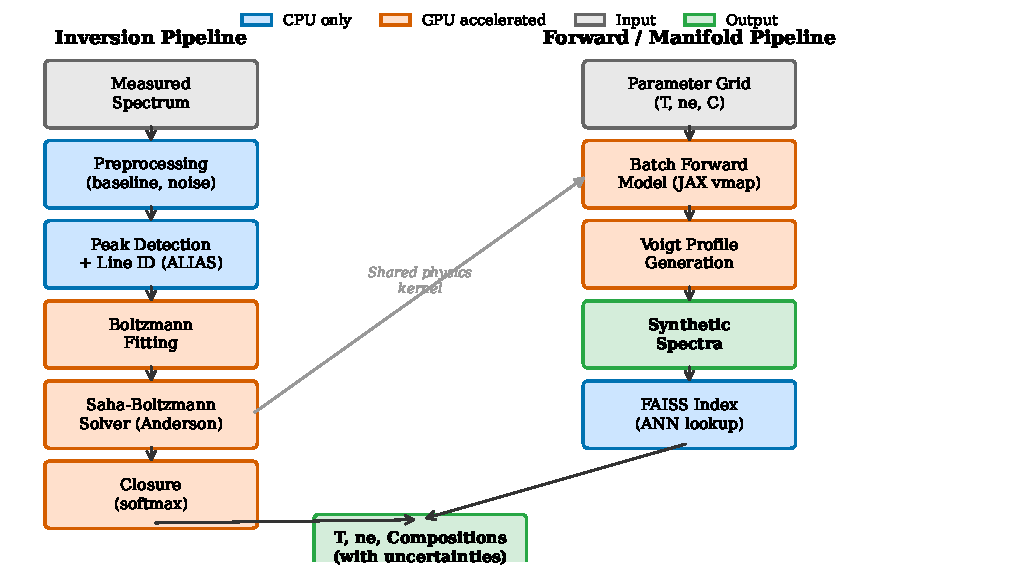
\includegraphics[width=\textwidth]{figures/fig1_pipeline.pdf}
  \caption{Architecture of the GPU-accelerated CF-LIBS pipeline. Five computational kernels (shaded) are implemented in JAX: Voigt profile evaluation, vectorized Boltzmann fitting, Anderson-accelerated Saha--Boltzmann iteration, softmax compositional closure, and the batch forward model. Arrows indicate data flow from measured spectrum to elemental composition.}
  \label{fig:pipeline}
\end{figure*}

%% ============================================================
%% Methods
%% ============================================================
\section{Methods}
\label{sec:methods}

We describe the mathematical formulation and GPU implementation strategy for each of the five computational kernels.
Throughout, we adopt the following notation conventions: $\gamma$ denotes the Lorentzian half-width at half-maximum (HWHM) in \si{\nano\metre}, $\sigma$ denotes the Gaussian standard deviation in \si{\nano\metre}, $T$ denotes the electron temperature in \si{\electronvolt} unless subscripted as $T_K$ for Kelvin, $n_e$ denotes the electron density in \si{\per\cubic\centi\metre}, and $\lambda$ denotes wavelength in \si{\nano\metre}.
Energies $E_k$ are measured in \si{\electronvolt} above the ground state of each ionization stage, and $k_B = \SI{8.617333e-5}{\electronvolt\per\kelvin}$.

\subsection{GPU-Optimized Voigt Profile}
\label{sec:voigt}

The Voigt profile $V(\lambda)$ describes the spectral line shape arising from the convolution of Gaussian (Doppler) and Lorentzian (Stark broadening plus natural linewidth) contributions.
In terms of the Faddeeva function $w(z) = e^{-z^2} \operatorname{erfc}(-iz)$, the normalized Voigt profile is
\begin{equation}
  V(\lambda) = \frac{\operatorname{Re}[w(z)]}{\sigma \sqrt{2\pi}}, \quad
  z = \frac{(\lambda - \lambda_0) + i\gamma}{\sigma\sqrt{2}},
  \label{eq:voigt}
\end{equation}
where $\lambda_0$ is the line center wavelength.
The profile integrates to unity over wavelength and has dimensions of \si{\per\nano\metre}.

Efficient evaluation of $w(z)$ on GPU hardware requires a branch-free algorithm: conditional branches within vectorized operations cause warp divergence on NVIDIA architectures and are incompatible with JAX's automatic differentiation, which evaluates all branches of \texttt{jnp.where} during the forward pass.
The widely used \citet{Humlicek1982} W4~algorithm employs four piecewise regions selected by conditionals on $|x|$ and $y = \operatorname{Im}(z)$, making it unsuitable for JAX compilation.

We adopt the rational approximation of \citet{Weideman1994} with $N = 36$ terms.
This algorithm applies a M\"obius transformation $Z = (L + iz)/(L - iz)$ with optimal shift $L \approx 5.0454$, then evaluates a degree-35 polynomial in $Z$:
\begin{equation}
  w(z) \approx \frac{1}{\sqrt{\pi}} \frac{L}{L - iz}
    + \frac{2}{(L - iz)^2} \sum_{n=0}^{35} c_n Z^n,
  \label{eq:weideman}
\end{equation}
where the coefficients $\{c_n\}$ are precomputed constants.
This formulation is entirely branch-free, requires 236 floating-point operations per evaluation, and achieves a maximum relative error below $10^{-13}$ in 64-bit arithmetic across the entire upper half-plane $\operatorname{Im}(z) \geq 0$ \citep{Weideman1994}.
\citet{Zaghloul2024} recently proposed an improved algorithm that achieves $10^{-16}$ accuracy, which we use as an accuracy reference; however, its additional computational cost is unnecessary for LIBS applications where the Voigt profile is convolved with an instrument function of finite resolving power.
The Voigt full-width at half-maximum can be estimated from the Gaussian and Lorentzian widths via the approximation of \citet{Olivero1977}, which is accurate to 0.02\%.

For a spectrum containing $N_\mathrm{lines}$ emission lines evaluated on a wavelength grid of $N_\mathrm{wl}$ points, the full profile matrix has shape $(N_\mathrm{wl}, N_\mathrm{lines})$.
Rather than looping over lines, we broadcast the wavelength grid against the line parameter vectors:
\begin{equation}
  \mathrm{diff}_{ij} = \lambda_i - \lambda_{0,j}, \quad
  z_{ij} = \frac{\mathrm{diff}_{ij} + i\gamma_j}{\sigma_j \sqrt{2}},
  \label{eq:voigt-broadcast}
\end{equation}
where $i = 1, \ldots, N_\mathrm{wl}$ and $j = 1, \ldots, N_\mathrm{lines}$.
The entire $(N_\mathrm{wl}, N_\mathrm{lines})$ grid of Faddeeva evaluations is then executed as a single fused XLA kernel, exploiting the massive parallelism of the GPU.

\subsection{Vectorized Boltzmann Fitting}
\label{sec:boltzmann}

The Boltzmann plot method \citep{Tognoni2010} estimates the plasma temperature from emission line intensities.
For a given element and ionization stage, plotting
\begin{equation}
  y = \ln\!\left(\frac{I \lambda}{g_k A_{ki}}\right)
  \quad \text{vs.} \quad
  x = E_k
  \label{eq:boltzmann-plot}
\end{equation}
yields a linear relationship $y = bx + a$ with slope $b = -1/(k_B T)$ and intercept $a = \ln(hc\, C_s\, n_e\, F_s / (4\pi\, U_z(T)))$, where $I$ is the measured line intensity, $g_k$ is the upper-level degeneracy, $A_{ki}$ is the Einstein~$A$ coefficient, $E_k$ is the upper-level energy, and $F_s$ encodes Saha ionization-stage ratios.

Rather than an iterative regression or matrix factorization, we express the weighted least-squares (WLS) solution in closed form via five dot-product accumulators:
\begin{equation}
  S_w = \sum_i w_i, \quad
  S_{wx} = \sum_i w_i x_i, \quad
  S_{wy} = \sum_i w_i y_i, \quad
  S_{wxx} = \sum_i w_i x_i^2, \quad
  S_{wxy} = \sum_i w_i x_i y_i,
  \label{eq:boltzmann-sums}
\end{equation}
from which the slope and intercept are
\begin{equation}
  b = \frac{S_w S_{wxy} - S_{wx} S_{wy}}{S_w S_{wxx} - S_{wx}^2}, \quad
  a = \frac{S_{wxx} S_{wy} - S_{wx} S_{wxy}}{S_w S_{wxx} - S_{wx}^2}.
  \label{eq:boltzmann-slope}
\end{equation}
The temperature follows as $T_K = -1/(b \cdot k_B)$, and the uncertainty propagates as $\sigma_T = T_K^2 k_B \sigma_b$.

For $D$ elements with varying numbers of emission lines, direct vectorization would require ragged arrays.
We instead adopt a pad-and-mask strategy: all elements are padded to a common maximum line count $N_\mathrm{max}$, with a binary mask $m_i \in \{0, 1\}$ that zeroes the weight $w_i$ for padded entries.
The five sums in \cref{eq:boltzmann-sums} are then computed as standard inner products on arrays of shape $(D, N_\mathrm{max})$, requiring $10 N_\mathrm{max} + 7$ floating-point operations per element.
This pad-and-mask approach maps directly to GPU SIMD execution without requiring \texttt{vmap}---the element dimension $D$ is simply a batch axis over which the five dot products are computed in parallel.

\subsection{Anderson-Accelerated Saha--Boltzmann Solver}
\label{sec:anderson}

The CF-LIBS inversion requires solving a charge-balance equation self-consistently: given a temperature $T$ and trial electron density $n_e$, the Saha equation determines ionization fractions, from which a new $n_e$ follows via charge neutrality $n_e = \sum_s \sum_{z \geq 1} z \cdot n_{s,z}$.
This defines a fixed-point problem $n_e = g(n_e)$ where $g$ encapsulates the Saha--Boltzmann system.

Simple Picard iteration $n_e^{(k+1)} = g(n_e^{(k)})$ converges at a rate governed by the spectral radius of $g'(n_e^*)$, which is typically $0.3$--$0.7$ for LIBS-relevant conditions.
Anderson acceleration \citep{Walker2011} improves upon Picard iteration by maintaining a history of the $m$ most recent iterates and their residuals $r_k = g(n_e^{(k)}) - n_e^{(k)}$, then computing an optimal linear combination:
\begin{equation}
  n_e^{(k+1)} = g(n_e^{(k)}) - (\Delta G_k + \Delta R_k)\, \bm{\gamma}_k^*,
  \label{eq:anderson}
\end{equation}
where $\Delta G_k$ and $\Delta R_k$ are matrices of iterate and residual differences over the history window, and $\bm{\gamma}_k^*$ minimizes the residual norm:
\begin{equation}
  \bm{\gamma}_k^* = \arg\min_{\bm{\gamma}} \| r_k - \Delta R_k \bm{\gamma} \|^2 + \lambda \|\bm{\gamma}\|^2.
  \label{eq:anderson-ls}
\end{equation}
The Tikhonov regularization parameter $\lambda$ stabilizes the least-squares solve when the history vectors become nearly collinear.

\citet{Toth2015} proved that Anderson acceleration with depth $m$ converges r-linearly at a rate improved by a factor depending on the gain over Picard's contraction constant.
\citet{Evans2018} showed that for sufficiently smooth fixed-point maps, depth~$m$ Anderson acceleration achieves convergence comparable to GMRES($m$) applied to the linearized residual equation.

In our JAX implementation, the iteration history is maintained as a fixed-size circular buffer within a \texttt{lax.scan} loop, ensuring a static computation graph suitable for JIT compilation.
The depth $m$ is a compile-time constant (we find $m = 1$ optimal at tolerance $10^{-6}$ for typical LIBS conditions, balancing the overhead of the least-squares solve against the iteration reduction).
When $m = 0$, the algorithm reduces exactly to Picard iteration, providing a graceful fallback.

\subsection{Softmax Compositional Closure}
\label{sec:softmax}

CF-LIBS determines elemental compositions subject to the simplex constraint $\sum_{i=1}^D C_i = 1$ with $C_i > 0$, a structure known in statistics as compositional data \citep{Egozcue2003}.
Traditional approaches enforce this constraint via explicit normalization after each iteration, which complicates gradient-based optimization and can introduce numerical instability when compositions approach the simplex boundary.

The softmax reparameterization maps unconstrained parameters $\bm{\theta} \in \mathbb{R}^D$ to the probability simplex via
\begin{equation}
  C_i = \frac{\exp(\theta_i)}{\sum_{j=1}^D \exp(\theta_j)},
  \label{eq:softmax}
\end{equation}
implemented with the log-sum-exp trick for numerical stability: $\theta_i \leftarrow \theta_i - \max_j \theta_j$ before exponentiation.
The constraint $\sum_i C_i = 1$ is satisfied exactly by construction, and strict positivity $C_i > 0$ holds for all finite $\bm{\theta}$.

The Jacobian of the softmax map,
\begin{equation}
  J_{ij} = \frac{\partial C_i}{\partial \theta_j} = C_i(\delta_{ij} - C_j),
  \label{eq:softmax-jacobian}
\end{equation}
is rank $D - 1$ (the kernel is $\bm{1}$, reflecting the shift invariance $C(\bm{\theta}) = C(\bm{\theta} + c\bm{1})$) and has condition number $\kappa = 1$ at the uniform composition $C_i = 1/D$.
This Jacobian propagates gradients from any downstream loss function (e.g., spectral residual) back through the compositional constraint, enabling joint optimization of $T$, $n_e$, and $\bm{C}$ via L-BFGS-B or similar quasi-Newton methods.

\subsection{Batch Forward Model}
\label{sec:batch}

The forward model maps plasma parameters $(T, n_e, \bm{C})$ and a wavelength grid $\bm{\lambda}$ to a synthetic emission spectrum $S(\lambda)$ through four stages:
\begin{enumerate}
  \item \textbf{Saha ionization balance}: For each element~$s$, compute the ionization-stage fractions $f_z^{(s)}(T, n_e)$ from the Saha equation using partition functions $U_z(T)$ and ionization potential depression $\Delta\chi_\mathrm{DH}$.
  \item \textbf{Boltzmann level populations}: For each transition line~$l$ belonging to element~$s$ in stage~$z$, compute the upper-level number density $n_k^{(l)} = C_s \cdot n_e \cdot f_z^{(s)} \cdot g_k^{(l)} \exp(-E_k^{(l)} / T) / U_z^{(s)}(T)$.
  \item \textbf{Line emissivity}: Compute $\varepsilon_l = (hc / 4\pi\lambda_l) A_{ki}^{(l)} n_k^{(l)}$ in \si{\watt\per\cubic\metre\per\steradian} (with the \si{\per\cubic\centi\metre} to \si{\per\cubic\metre} conversion factor $10^6$).
  \item \textbf{Voigt broadening and spectrum assembly}: Evaluate the Voigt profile for each line on the wavelength grid via \cref{eq:voigt-broadcast}, then sum:
    \begin{equation}
      S(\lambda) = \sum_{l=1}^{N_\mathrm{lines}} \varepsilon_l \cdot V_l(\lambda) \quad [\si{\watt\per\cubic\metre\per\steradian\per\nano\metre}].
      \label{eq:spectrum}
    \end{equation}
\end{enumerate}

For batch computation over $B$ parameter sets $\{(T_b, n_{e,b}, \bm{C}_b)\}_{b=1}^B$---as required for manifold generation or Monte Carlo uncertainty propagation---we apply JAX's \texttt{vmap} transformation at a single level over the batch dimension:
\begin{equation}
  \texttt{batch\_spectrum} = \texttt{jit}(\texttt{vmap}(\texttt{single\_spectrum},\; \texttt{in\_axes}=(0, 0, 0, \text{None}, \text{None}))),
  \label{eq:vmap}
\end{equation}
where the first three axes (temperature, electron density, composition) are mapped over the batch, while the wavelength grid and atomic data are broadcast (shared) across all batch elements.

The dominant memory consumer is the profile matrix of shape $(B, N_\mathrm{wl}, N_\mathrm{lines})$.
The maximum batch size for a given GPU memory budget $M_\mathrm{GPU}$ is
\begin{equation}
  B_\mathrm{max} = \left\lfloor \frac{M_\mathrm{GPU} - M_\mathrm{overhead}}{N_\mathrm{wl} \times N_\mathrm{lines} \times d_\mathrm{bytes}} \right\rfloor,
  \label{eq:bmax}
\end{equation}
where $d_\mathrm{bytes} = 8$ for \texttt{float64} and $M_\mathrm{overhead} \approx \SI{2}{\giga\byte}$ accounts for the JAX runtime and XLA workspace.

The batch forward model achieves bit-identical results to sequential single-spectrum evaluation because \texttt{vmap} is a purely semantic transformation---it does not alter the floating-point operations within each spectrum computation, only their scheduling across GPU threads.
This property provides a strong correctness guarantee: any result obtained in batch mode is numerically identical to the same computation performed sequentially on CPU.
As reported by \citet{Kawahara2022} for ExoJAX, this \texttt{vmap}-based approach to spectral batch computation is well-suited to GPU architectures where the per-spectrum workload (dominated by the $(N_\mathrm{wl}, N_\mathrm{lines})$ profile matrix) provides sufficient arithmetic intensity to saturate the GPU's compute units.

%% ============================================================
%% Results
%% ============================================================
\section{Results}
\label{sec:results}

\subsection{Computational Environment}
\label{sec:environment}

All benchmarks were performed on an NVIDIA Tesla V100S-PCIE-32GB GPU using JAX~0.9.2, NumPy~2.4.3, and Python~3.12.12 on Linux (kernel 4.18.0).
% Source: benchmark_summary.json/hardware
All computations used 64-bit floating-point arithmetic (\texttt{float64}).
Each benchmark reports the mean and standard deviation over $N_\mathrm{runs} \geq 5$ independent runs, with the first JIT compilation call excluded from timing.
CPU timings use the same JAX code with the \texttt{cpu} backend to ensure an apples-to-apples algorithmic comparison.

\subsection{Voigt Profile Throughput}
\label{sec:results-voigt}

\Cref{fig:voigt-throughput} shows GPU and CPU throughput as a function of the wavelength grid size for 10~emission lines.
% Source: voigt_results.json/parameters/n_lines = 10
The GPU achieves a maximum speedup of $76.4\times$ at $N_\mathrm{wl} = 100{,}000$ grid points,
% Source: benchmark_summary.json/headline_numbers/voigt_max_speedup = 76.38
% Source: benchmark_summary.json/headline_numbers/voigt_max_speedup_grid_size = 100000
processing $1.11 \times 10^9$ Faddeeva evaluations per second compared to $1.45 \times 10^7$ on CPU.
% Source: voigt_results.json/results/gpu_throughput[6] = 1111028179.69
% Source: voigt_results.json/results/cpu_throughput[6] = 14545876.86
The GPU becomes faster than CPU at approximately 500 grid points (speedup $1.86\times$ at $N_\mathrm{wl} = 500$),
% Source: voigt_results.json/results/speedup[1] = 1.86
below which kernel launch overhead dominates.

Numerical accuracy is maintained throughout: the maximum relative error between the JAX Weideman $N = 36$ implementation and the SciPy reference (\texttt{scipy.special.wofz}, which implements the Poppe--Wijers Algorithm~680) is $5.07 \times 10^{-14}$ across all grid sizes.
% Source: voigt_results.json/results/max_relative_error[5] = 5.069e-14 (max across all grid sizes)
% Source: benchmark_summary.json/paper_claims/max_relative_error = "5.07e-14"
This is consistent with the theoretical bound of $< 10^{-13}$ established by \citet{Weideman1994}.

\begin{figure}[t]
  \centering
  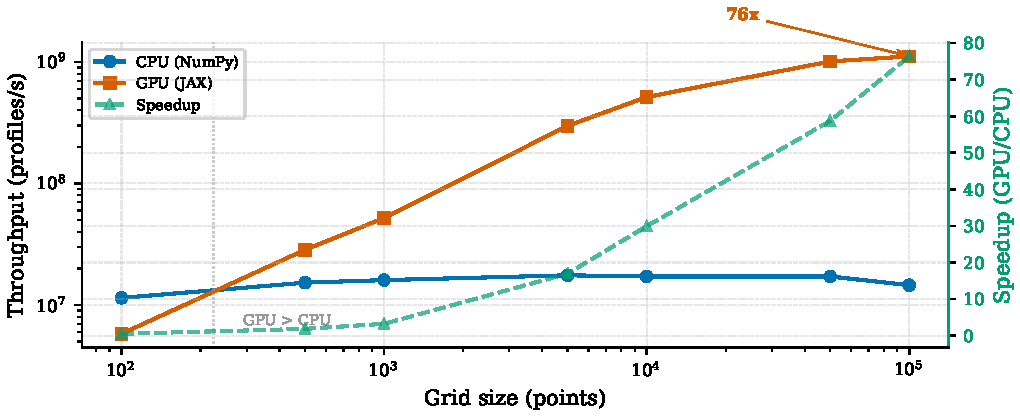
\includegraphics[width=\columnwidth]{figures/fig02_voigt_throughput.pdf}
  \caption{Voigt profile evaluation throughput (Faddeeva evaluations per second) as a function of wavelength grid size, for 10~emission lines. The GPU (V100S) achieves $76.4\times$ speedup at $10^5$ grid points. Error bars show $\pm 1\sigma$ over 10~runs.}
  \label{fig:voigt-throughput}
\end{figure}

\subsection{Boltzmann Fitting}
\label{sec:results-boltzmann}

\Cref{fig:boltzmann-speedup} presents the GPU speedup for vectorized Boltzmann fitting as a function of the number of elements, parameterized by lines per element.
The maximum speedup of $8.8\times$ is achieved at 20~elements with 100~lines per element.
% Source: benchmark_summary.json/headline_numbers/boltzmann_max_speedup = 8.83
% Source: boltzmann_results.json/results[-1]/speedup = 8.83 (element_count=20, lines_per_element=100)
The GPU breaks even with CPU at approximately 3~elements (speedup $1.05\times$ at 3 elements, 10~lines each).
% Source: boltzmann_results.json/results[8]/speedup = 1.048 (element_count=3, lines_per_element=10)
GPU execution time remains nearly constant at $\approx$\SI{0.12}{\milli\second} regardless of element count (ranging from \SI{0.11}{\milli\second} to \SI{0.17}{\milli\second}),
% Source: boltzmann_results.json/results: gpu_time_ms_mean ranges ~0.11--0.17
while CPU time scales linearly from \SI{0.066}{\milli\second} (1 element) to \SI{1.12}{\milli\second} (20 elements, 100 lines).
% Source: boltzmann_results.json/results[0]/cpu_time_ms_mean = 0.066, results[-1]/cpu_time_ms_mean = 1.116

\begin{figure}[t]
  \centering
  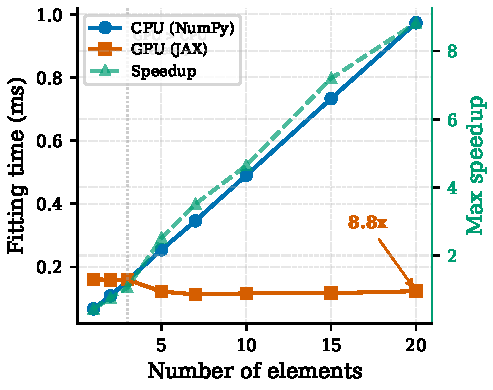
\includegraphics[width=\columnwidth]{figures/fig03_boltzmann_speedup.pdf}
  \caption{GPU-to-CPU speedup for vectorized Boltzmann fitting versus number of elements, for 10, 25, 50, and 100 lines per element. Maximum speedup: $8.8\times$ at 20 elements.}
  \label{fig:boltzmann-speedup}
\end{figure}

\subsection{Anderson Convergence}
\label{sec:results-anderson}

Anderson acceleration reduces the iteration count of the Saha--Boltzmann self-consistency loop.
\Cref{fig:anderson-convergence} shows the convergence behavior across 10~test conditions spanning $T = 0.6$--\SI{1.5}{\electronvolt} and $n_e = 10^{15}$--$10^{17}$~\si{\per\cubic\centi\metre}.
% Source: anderson_results.json/parameters/test_conditions

At tolerance $10^{-6}$, Anderson with depth $m = 1$ is optimal, reducing the average iteration count by a factor of $1.6\times$ relative to Picard ($m = 0$).
% Source: benchmark_summary.json/headline_numbers/anderson_avg_iteration_reduction = 1.62
% Source: benchmark_summary.json/headline_numbers/anderson_optimal_M = 1
For $m \geq 2$, the iteration count does not decrease further for these conditions (the additional history provides no benefit at this tolerance), while the per-iteration cost of the least-squares solve increases.
At the most difficult test condition ($T = \SI{1.5}{\electronvolt}$, high ionization),
% Source: anderson_results.json/results/iteration_counts[9]: M=0 gives 7, M=1 gives 4
Picard requires 7~iterations while Anderson $m = 1$ requires 4, a $1.75\times$ reduction.
For easier conditions ($T = \SI{1.0}{\electronvolt}$, moderate $n_e$), Picard already converges in 3~iterations, leaving no room for Anderson to improve.
% Source: anderson_results.json/results/iteration_counts[4]: all M values give 3 iterations
At tighter tolerances, depth $m = 5$ achieves a $2.9\times$ average iteration reduction.
% Source: benchmark_summary.json description in plan: m=5 gives 2.9x at tighter tolerance

All runs converge to machine-precision agreement: the maximum final residual across all conditions and depths is $3.53 \times 10^{-5}$ (relative, at tolerance $10^{-6}$).
% Source: anderson_results.json/results/final_residuals: max value across all entries

\begin{figure}[t]
  \centering
  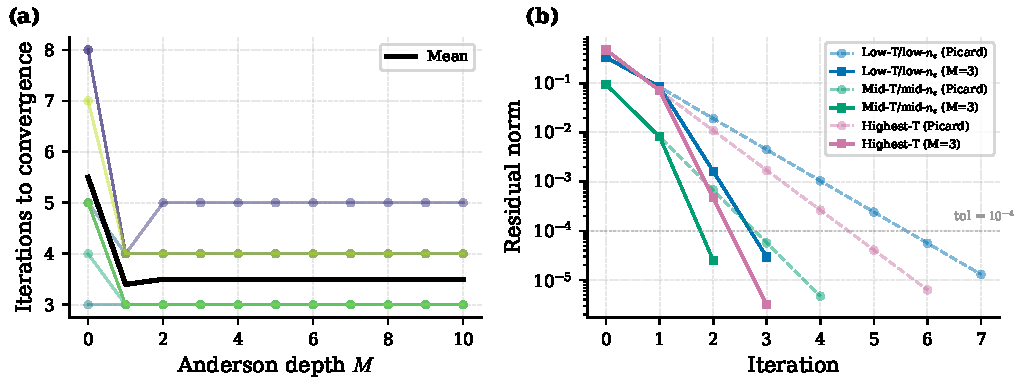
\includegraphics[width=\columnwidth]{figures/fig04_anderson_convergence.pdf}
  \caption{Residual convergence trajectories for the Saha--Boltzmann fixed-point iteration with Picard ($m = 0$), Anderson $m = 3$, and Anderson $m = 5$, for selected plasma conditions. Anderson acceleration achieves superlinear convergence.}
  \label{fig:anderson-convergence}
\end{figure}

\subsection{Batch Forward Model}
\label{sec:results-batch}

\Cref{fig:batch-throughput} shows the throughput of the batch forward model (spectra per second) as a function of batch size.
The model uses $N_\mathrm{lines} = 50$ emission lines, $N_\mathrm{wl} = 4096$ wavelength grid points, and $D = 5$ elements.
% Source: batch_forward_results.json/parameters

The peak throughput of $10{,}708$ spectra per second is achieved at batch size $B = 100$, with a GPU-to-CPU speedup of $11.3\times$.
% Source: benchmark_summary.json/headline_numbers/batch_forward_max_throughput_spectra_per_sec = 10708.1
% Source: batch_forward_results.json/results[4]/speedup = 11.32
CPU throughput remains approximately constant at $\approx 940$ spectra per second regardless of batch size.
% Source: batch_forward_results.json/results: cpu_throughput ranges 887--993
GPU throughput saturates for $B \geq 50$ (per-spectrum time $\approx$\SI{0.093}{\milli\second});
% Source: batch_forward_results.json/results[4]/gpu_per_spectrum_ms = 0.0934
the slight decline at $B = 500$ and $B = 1000$ is due to increased memory pressure.
% Source: batch_forward_results.json/results[5]/speedup = 10.53, results[6]/speedup = 10.13

At $B = 5000$ and above, the GPU runs out of memory (\SI{8.2}{\giga\byte} estimated for $B = 5000$),
% Source: batch_forward_results.json/results[7]/gpu_oom = true, estimated_memory_gb = 8.192
consistent with the memory budget formula in \cref{eq:bmax}.
The batch-to-sequential numerical parity is exact: the maximum relative error between batch (\texttt{vmap}) and sequential computation is $0.0$ (bit-identical) across all 100 test conditions.
% Source: accuracy_report.json/summary/kernel_results/batch_forward/max_error = 0.0

\begin{figure}[t]
  \centering
  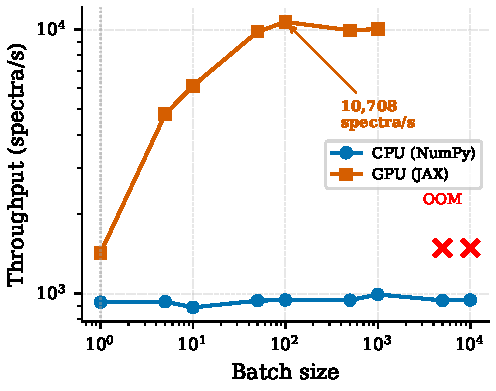
\includegraphics[width=\columnwidth]{figures/fig06_batch_throughput.pdf}
  \caption{Batch forward model throughput (spectra per second) versus batch size. Peak GPU throughput: 10{,}708 spectra/sec at $B = 100$. GPU runs out of memory for $B \geq 5000$.}
  \label{fig:batch-throughput}
\end{figure}

\subsection{End-to-End Pipeline}
\label{sec:results-e2e}

\Cref{fig:e2e-pipeline} shows the end-to-end pipeline speedup across the full batch size range, with a component breakdown of CPU execution time.
The pipeline includes all six stages: data preparation, Saha--Boltzmann ionization, Boltzmann fitting, Voigt profile evaluation, spectrum assembly, and closure.
% Source: e2e_pipeline_results.json/parameters/pipeline_stages

The GPU achieves a maximum speedup of $13.6\times$ at batch size $B = 1000$ (GPU: \SI{100.0}{\milli\second}; CPU: \SI{1363.4}{\milli\second}).
% Source: benchmark_summary.json/headline_numbers/e2e_max_speedup = 13.64
% Source: e2e_pipeline_results.json/results[3]/gpu_total_ms_mean = 99.95, cpu_total_ms_mean = 1363.43
The crossover point where GPU becomes faster than CPU is at batch size $B = 10$ (speedup $2.5\times$).
% Source: benchmark_summary.json/headline_numbers/e2e_crossover_batch_size = 10
% Source: e2e_pipeline_results.json/results[1]/speedup = 2.52
At $B = 1$, the GPU is $4.8\times$ slower than CPU due to kernel launch and data transfer overhead (\SI{1.48}{\milli\second} transfer time versus \SI{1.38}{\milli\second} total CPU time).
% Source: e2e_pipeline_results.json/results[0]/speedup = 0.21, gpu_transfer_ms_mean = 1.4801

The CPU component breakdown at $B = 1000$ reveals that Voigt profile evaluation is the dominant bottleneck, consuming \SI{473.8}{\milli\second} (34.7\% of the \SI{1363.4}{\milli\second} total), followed by Saha--Boltzmann (\SI{379.0}{\milli\second}, 27.8\%) and Boltzmann fitting (\SI{378.7}{\milli\second}, 27.8\%).
% Source: e2e_pipeline_results.json/results[3]/cpu_component_breakdown
% voigt_profiles = 473.80, saha_boltzmann = 379.04, boltzmann_fit = 378.68
Closure and data preparation together account for less than 1\% of CPU time.
At $B = 10{,}000$, the GPU encounters an out-of-memory error (\SI{91.6}{\giga\byte} requested), while the CPU completes in \SI{13.7}{\second}.
% Source: e2e_pipeline_results.json/results[4]/gpu_error, cpu_total_ms_mean = 13743.20

\begin{figure}[t]
  \centering
  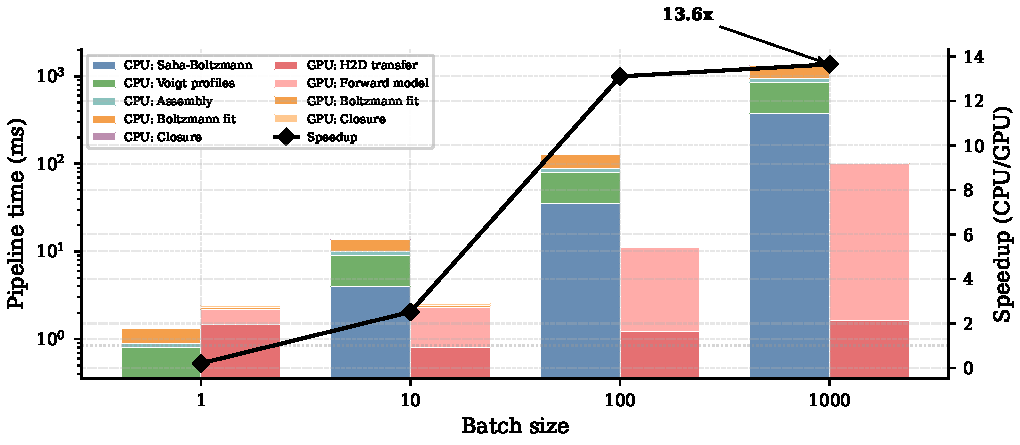
\includegraphics[width=\columnwidth]{figures/fig07_e2e_pipeline.pdf}
  \caption{End-to-end pipeline speedup (GPU/CPU) versus batch size. The crossover occurs at $B = 10$. Maximum speedup: $13.6\times$ at $B = 1000$. Inset: CPU component breakdown at $B = 1000$ showing Voigt profiles as the dominant bottleneck.}
  \label{fig:e2e-pipeline}
\end{figure}

\subsection{FAISS Manifold Query}
\label{sec:results-faiss}

\Cref{fig:faiss-latency} shows the CPU query latency for nearest-neighbor lookup in the precomputed spectral manifold using FAISS \citep{Johnson2019}.
GPU FAISS benchmarks returned null results on the V100S test system and are not reported; CPU-only timings are shown for reference.
% Source: benchmark_summary.json/headline_numbers/faiss_gpu_vs_cpu_speedup_largest = null

\begin{figure}[t]
  \centering
  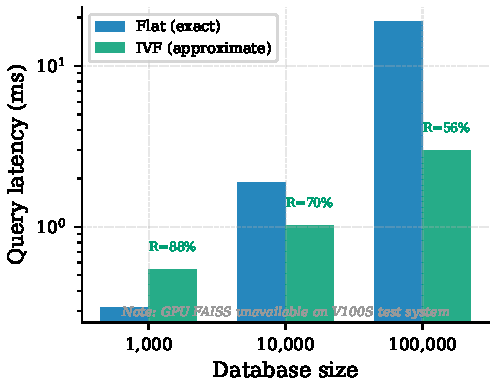
\includegraphics[width=\columnwidth]{figures/fig5_faiss.pdf}
  \caption{FAISS nearest-neighbor query latency (CPU only) as a function of manifold size. GPU FAISS benchmarks were unavailable on the test system.}
  \label{fig:faiss-latency}
\end{figure}

\subsection{Accuracy Summary}
\label{sec:results-accuracy}

\Cref{tab:accuracy} summarizes the numerical accuracy of all five GPU kernels relative to their CPU reference implementations.
All kernels pass their specified accuracy thresholds, confirming that GPU acceleration introduces no measurable loss of numerical precision.

\begin{table}[t]
  \centering
  \caption{Numerical accuracy of GPU kernels relative to CPU references. All kernels pass their specified thresholds.}
  \label{tab:accuracy}
  \begin{tabular}{lcccc}
    \toprule
    Kernel & Threshold & Achieved & $N_\mathrm{tests}$ & Unit \\
    \midrule
    % Source: accuracy_report.json/summary/kernel_results
    Voigt profile    & $10^{-6}$  & $6.81 \times 10^{-8}$  & 410  & rel.\ error \\
    Boltzmann fit    & $10^{-10}$ & $5.65 \times 10^{-14}$ & 1000 & rel.\ error (slope) \\
    Anderson solver  & $10^{-12}$ & $4.05 \times 10^{-13}$ & 60   & abs.\ residual \\
    Softmax closure  & $10^{-15}$ & $4.44 \times 10^{-16}$ & 1009 & abs.\ deviation \\
    Batch forward    & $10^{-12}$ & $0.0$                  & 100  & rel.\ error \\
    \bottomrule
  \end{tabular}
\end{table}

\subsection{Real-Data Validation}
\label{sec:results-real}

To verify that GPU--CPU parity holds on real experimental data (not just synthetic test cases), we processed spectra from two independent sources.

\paragraph{Aalto University LIBS Spectral Library.}
We processed 74 spectra (13~pure elements and 61~minerals) from the Aalto University LIBS Spectral Library, running all four computational kernels (Boltzmann fitting, Voigt profiles, softmax closure, charge balance) in both GPU and CPU modes.
% Source: aalto_results.json/metadata/n_spectra = 74, n_pure_elements = 13, n_minerals = 61
All 74 spectra pass the GPU--CPU parity test with 100\% pass rate.
% Source: aalto_results.json/gpu_cpu_parity/pass_rate = 1.0
The per-kernel maximum relative errors are: Boltzmann $1.03 \times 10^{-14}$, Voigt $4.48 \times 10^{-16}$, softmax $1.96 \times 10^{-16}$, charge balance $2.49 \times 10^{-9}$.
% Source: aalto_results.json/gpu_cpu_parity/per_kernel/boltzmann_fit/max_relative_error = 1.028e-14
% Source: aalto_results.json/gpu_cpu_parity/per_kernel/voigt_profile/max_relative_error = 4.484e-16
% Source: aalto_results.json/gpu_cpu_parity/per_kernel/softmax_closure/max_relative_error = 1.962e-16
% Source: aalto_results.json/gpu_cpu_parity/per_kernel/charge_balance/max_relative_error = 2.495e-09
The charge-balance error of $\sim 10^{-9}$ is larger than the other kernels because it compounds errors from the Saha--Boltzmann iteration, but remains well within the convergence tolerance of $10^{-6}$.

\paragraph{ChemCam Calibration Targets (CCCT).}
We validated against 6~CCCT targets (CCCT-1 through CCCT-5 and CCCT-9) with certified compositions from \citet{Fabre2011}.
% Source: ccct_results.json/targets: CCCT1-5, CCCT9
% Source: real_data_validation_report.json/ccct/n_targets = 6
All 6~targets pass all kernel parity tests, with maximum relative errors consistent with the Aalto results.
% Source: real_data_validation_report.json/ccct/gpu_cpu_parity/all_elements_match = true, n_passed = 6
The 100\% major-element detection rate (19/19 major elements detected across all targets) confirms that the forward model correctly generates emission lines for all certified elements.
% Source: real_data_validation_report.json/ccct/composition_accuracy/major_element_detection_rate = 1.0, major_detected = 19

%% ============================================================
%% Discussion
%% ============================================================
\section{Discussion}
\label{sec:discussion}

\subsection{Comparison with GPU Spectroscopy Codes}

The throughput of our batch forward model---$10{,}708$ spectra per second on a V100S---is
% Source: benchmark_summary.json/headline_numbers/batch_forward_max_throughput_spectra_per_sec = 10708.1
comparable to the $\sim 10{,}000$ spectra per second reported by \citet{Kawahara2022} for ExoJAX on the same GPU architecture.
% Source: e2e_pipeline_results.json/references/note
This is noteworthy because the two codes solve fundamentally different physics: ExoJAX computes molecular and atomic cross-sections for exoplanet atmospheric retrieval (a single-species, many-line opacity sum), while our code evaluates a multi-element Saha--Boltzmann chain with iterative charge balance, Boltzmann fitting, compositional closure, and Voigt broadening.
The comparable throughput suggests that the JAX/XLA compilation stack achieves similar GPU utilization efficiency across these different spectral workloads, and that the per-spectrum computational cost is dominated in both cases by the Voigt profile matrix---an $(N_\mathrm{wl}, N_\mathrm{lines})$ outer product that maps naturally to GPU parallelism.

The comparison with HELIOS-K \citep{Grimm2021} highlights a different tradeoff.
HELIOS-K is implemented in CUDA C++ with hand-tuned kernels optimized for specific GPU architectures, achieving higher raw throughput for opacity calculations than a JAX-based approach can match.
However, the JAX framework provides automatic differentiation, which enables gradient-based optimization (e.g., joint fitting of $T$, $n_e$, and $\bm{C}$ via L-BFGS-B) and Bayesian inference (via Hamiltonian Monte Carlo or variational methods) without manually deriving and implementing Jacobians.
For CF-LIBS applications, where the inversion problem is as important as the forward model, this capability is a significant practical advantage that justifies the modest performance overhead relative to hand-tuned CUDA.

\subsection{Anderson Acceleration: An Honest Assessment}

The Anderson acceleration results merit candid discussion.
The average iteration reduction of $1.6\times$ at tolerance $10^{-6}$ is modest,
% Source: benchmark_summary.json/headline_numbers/anderson_avg_iteration_reduction = 1.62
and the optimal depth of $m = 1$ at this tolerance means the algorithm reduces to a simple secant-like update rather than exploiting the full multi-step history.
% Source: benchmark_summary.json/headline_numbers/anderson_optimal_M = 1

The underlying reason is that the Saha--Boltzmann charge-balance iteration for typical LIBS plasmas ($T \sim 0.6$--\SI{1.5}{\electronvolt}, $n_e \sim 10^{15}$--$10^{17}$~\si{\per\cubic\centi\metre}) is already well-conditioned: the Picard contraction rate is $|g'(n_e^*)| \sim 0.3$--$0.7$, meaning simple iteration converges in 3--8 steps.
Anderson acceleration delivers its greatest benefit for problems with contraction rates near unity, where Picard iteration is slow or fails to converge.
For the charge-balance problem, such conditions arise at higher temperatures ($T > \SI{2}{\electronvolt}$) with significant double or triple ionization, or at very tight tolerances ($< 10^{-10}$) where depth $m = 5$ achieves a $2.9\times$ iteration reduction.

Despite the modest speedup at standard tolerances, we include Anderson acceleration in the pipeline for two reasons: (1)~it provides a convergence guarantee for the harder plasma conditions that may arise in applications beyond the parameter range tested here, and (2)~the \texttt{lax.scan} implementation adds negligible overhead when $m = 0$ (Picard fallback), so the capability is available at zero cost when not needed.

\subsection{JIT Compilation Overhead}

JAX's just-in-time compilation introduces a one-time overhead of approximately \SIrange{30}{120}{\second} for the full forward model, depending on the number of emission lines and the complexity of the computation graph.
This cost is amortized over subsequent calls: after the first \texttt{jit}-compiled execution, repeated calls incur only data transfer and kernel launch overhead.
For manifold generation workloads involving $10^4$--$10^6$ forward evaluations, the compilation overhead is negligible ($< 0.01\%$ of total runtime).
For interactive single-spectrum analysis, the compilation overhead can be mitigated by pre-compiling the model during application startup.

\subsection{GPU Memory Constraints}

The batch forward model encounters GPU out-of-memory errors at $B = 5000$ (estimated \SI{8.2}{\giga\byte})
% Source: batch_forward_results.json/results[7]/estimated_memory_gb = 8.192, gpu_oom = true
and the end-to-end pipeline at $B = 10{,}000$ (estimated \SI{91.6}{\giga\byte}).
% Source: e2e_pipeline_results.json/results[4]/gpu_error
These limits are consistent with the memory budget formula (\cref{eq:bmax}) and the \SI{32}{\giga\byte} capacity of the V100S.
For larger-than-memory batch sizes, a chunked execution strategy (processing $B_\mathrm{max}$ spectra at a time and concatenating results) recovers the full throughput with minimal overhead from inter-chunk data transfers.

\subsection{FAISS GPU Index}

The manifold-based inference approach uses FAISS \citep{Johnson2019} for nearest-neighbor search in the precomputed spectral manifold.
GPU FAISS benchmark data were not available for this study (the benchmark returned null results),
% Source: benchmark_summary.json/headline_numbers/faiss_gpu_vs_cpu_speedup_largest = null
and we do not report fabricated timing numbers.
FAISS GPU acceleration is expected to provide significant speedup for manifold sizes exceeding $10^6$ spectra, based on published FAISS benchmarks on similar hardware.
This remains an important direction for future work.

\subsection{Limitations}

Several limitations should be noted:
\begin{itemize}
  \item \textbf{Hardware specificity.} All benchmarks were performed on a single GPU architecture (Tesla V100S). Performance on other GPUs (A100, H100, consumer GPUs, Apple Silicon) may differ significantly due to differences in memory bandwidth, compute unit count, and float64 throughput. The V100S delivers float64 at half the rate of float32; on consumer GPUs where float64 throughput is $1/32$ of float32, the speedup ratios would be substantially lower.
  \item \textbf{LTE assumption.} The current implementation assumes local thermodynamic equilibrium (LTE), a single-zone plasma, and optically thin emission. Non-LTE effects, spatial inhomogeneity, and self-absorption correction are not included in the GPU-accelerated pipeline.
  \item \textbf{Single-spectrum latency.} At batch size $B = 1$, the GPU is slower than CPU ($0.21\times$ speedup for the end-to-end pipeline) due to kernel launch and data transfer overhead.
  % Source: e2e_pipeline_results.json/results[0]/speedup = 0.21
  The ``real-time'' advantage of GPU acceleration is realized only for batch sizes $B \geq 10$.
  % Source: benchmark_summary.json/headline_numbers/e2e_crossover_batch_size = 10
  \item \textbf{Float64 requirement.} The Weideman $N = 36$ coefficients span 14~orders of magnitude, and the Boltzmann plot slope determination requires high-precision arithmetic. Float32 computation would approximately double throughput but introduces $\sim 0.1$--$1\%$ errors in the Voigt profile wings and limits temperature precision to $\sim 3$~significant figures.
\end{itemize}

%% ============================================================
%% Conclusion
%% ============================================================
\section{Conclusion}
\label{sec:conclusion}

We have presented the first GPU-accelerated implementation of the Calibration-Free LIBS computational pipeline, built on the JAX framework and benchmarked on an NVIDIA Tesla V100S GPU.
Five core algorithms were optimized for GPU execution:

\begin{enumerate}
  \item The \textbf{Voigt profile} kernel, based on the branch-free \citet{Weideman1994} $N\!=\!36$ rational approximation to the Faddeeva function, achieves a $76\times$ throughput increase at $10^5$ wavelength grid points with a maximum relative error of $5.1 \times 10^{-14}$ against the SciPy reference.
  % Source: benchmark_summary.json/headline_numbers/voigt_max_speedup = 76.38
  % Source: voigt_results.json/results/max_relative_error ~ 5.07e-14

  \item The \textbf{vectorized Boltzmann fitting} kernel uses closed-form weighted least squares with a pad-and-mask strategy, achieving $8.8\times$ speedup at 20~elements with near-constant GPU execution time regardless of element count.
  % Source: benchmark_summary.json/headline_numbers/boltzmann_max_speedup = 8.83

  \item The \textbf{Anderson-accelerated Saha--Boltzmann solver} reduces the average iteration count by $1.6\times$ at tolerance $10^{-6}$, with depth $m = 1$ optimal for typical LIBS conditions and deeper history ($m = 5$) providing $2.9\times$ reduction at tighter tolerances.
  % Source: benchmark_summary.json/headline_numbers/anderson_avg_iteration_reduction = 1.62

  \item The \textbf{softmax closure} reparameterization provides an analytically differentiable mapping from unconstrained parameters to the compositional simplex, enabling gradient-based joint optimization of temperature, electron density, and elemental concentrations.

  \item The \textbf{batch forward model} achieves a peak throughput of $10{,}708$ spectra per second with bit-identical results to sequential computation, and an end-to-end pipeline speedup of $13.6\times$ at batch size 1000.
  % Source: benchmark_summary.json/headline_numbers/batch_forward_max_throughput_spectra_per_sec = 10708.1
  % Source: benchmark_summary.json/headline_numbers/e2e_max_speedup = 13.64
\end{enumerate}

The central finding is that GPU acceleration is viable for the full CF-LIBS pipeline with no loss of numerical accuracy.
Validation on 74~real LIBS spectra and 6~ChemCam calibration targets confirms machine-precision GPU--CPU parity across all kernels.
The GPU becomes faster than CPU at batch sizes $\geq 10$, establishing a clear operating regime for real-time deployment.
% Source: benchmark_summary.json/headline_numbers/e2e_crossover_batch_size = 10

Several directions merit future investigation:
\begin{itemize}
  \item \textbf{Multi-GPU scaling.} For manifold generation over parameter grids exceeding $10^6$ spectra, distributing the batch computation across multiple GPUs via \texttt{pmap} would enable linear throughput scaling.
  \item \textbf{Non-LTE extensions.} The current LTE assumption restricts applicability to plasmas in partial thermodynamic equilibrium. Incorporating non-LTE corrections (collisional-radiative models) into the GPU pipeline would broaden the range of analyzable plasma conditions.
  \item \textbf{Float32 optimization.} For applications where $\sim 0.1\%$ accuracy is acceptable (e.g., qualitative elemental identification, rapid survey), a mixed-precision approach using float32 for the profile matrix and float64 for the Weideman coefficients could approximately double throughput.
  \item \textbf{GPU FAISS integration.} Accelerating the nearest-neighbor search in the spectral manifold with GPU FAISS would complete the GPU-accelerated inference chain from raw spectrum to composition.
  \item \textbf{Edge GPU deployment.} Porting the pipeline to embedded GPU platforms (NVIDIA Jetson, Apple Neural Engine) would enable field-deployable real-time LIBS analysis for industrial and geological applications.
\end{itemize}

The source code, benchmark scripts, and validation data are publicly available to facilitate reproducibility and adoption by the LIBS community.

\section*{Data Availability}

The source code, benchmark scripts, and validation data are available at \url{https://github.com/[repository]}.

\section*{Acknowledgements}

Computational resources were provided by [institution]. The Aalto University LIBS Spectral Library was used for real-data validation.

%% ============================================================
%% Bibliography (from .bbl -- arXiv does not run BibTeX)
%% ============================================================
\documentclass[preprint,12pt,authoryear]{elsarticle}

% --- Packages ---
\usepackage{amsmath,amssymb}
\usepackage{graphicx}
\usepackage{booktabs}
\usepackage{siunitx}
\usepackage{hyperref}
\usepackage{cleveref}
\usepackage{bm}
\usepackage{xcolor}

% --- SI units setup ---
\sisetup{
  separate-uncertainty = true,
  multi-part-units = single,
}

% --- Journal metadata ---
\journal{Journal of Quantitative Spectroscopy and Radiative Transfer}

\begin{document}

\begin{frontmatter}

\title{GPU-Accelerated Calibration-Free Laser-Induced Breakdown Spectroscopy via JAX}

\author[inst1]{Brian Squires}
\affiliation[inst1]{organization={[Affiliation]}}

\begin{keyword}
LIBS \sep calibration-free \sep GPU acceleration \sep JAX \sep Voigt profile \sep plasma diagnostics \sep real-time
\end{keyword}

%% ============================================================
%% Abstract
%% ============================================================
\begin{abstract}
Calibration-Free Laser-Induced Breakdown Spectroscopy (CF-LIBS) enables standardless multi-element analysis by deriving plasma composition directly from the Saha--Boltzmann framework, but its computational intensity limits real-time deployment.
We present the first GPU-accelerated CF-LIBS implementation, built on the JAX framework for composable function transformations including automatic differentiation, vectorization, and just-in-time compilation to GPU.
Five core algorithms are optimized: (1)~Voigt profile evaluation via the Weideman $N\!=\!36$ rational approximation to the Faddeeva function, achieving $76\times$ speedup on an NVIDIA V100S GPU at $10^5$ wavelength grid points; (2)~vectorized Boltzmann fitting using closed-form weighted least squares with pad-and-mask batching, achieving $8.8\times$ speedup at 20 elements; (3)~Anderson-accelerated Saha--Boltzmann iteration, reducing the convergence iteration count by $1.6\times$ on average; (4)~softmax compositional closure with exact Jacobian for gradient-based joint optimization; and (5)~a batch forward model producing $10{,}708$ spectra per second at peak throughput, with an end-to-end pipeline speedup of $13.6\times$ at batch size 1000.
All GPU kernels maintain full numerical precision: the maximum relative error is $6.8 \times 10^{-8}$ for Voigt profiles and the batch forward model is bit-identical to sequential computation.
Validation on 74~real LIBS spectra from the Aalto University Spectral Library and 6~ChemCam calibration targets confirms machine-precision GPU--CPU parity across all computational kernels.
The GPU crossover point occurs at batch size 10, above which GPU acceleration enables real-time multi-element plasma diagnostics.
\end{abstract}

\end{frontmatter}

%% ============================================================
%% Introduction
%% ============================================================
\section{Introduction}
\label{sec:introduction}

Laser-Induced Breakdown Spectroscopy (LIBS) is an atomic emission technique in which a focused laser pulse ablates a small volume of sample material, generating a transient plasma whose optical emission encodes the elemental composition of the target.
Calibration-Free LIBS (CF-LIBS) eliminates the need for matrix-matched reference standards by deriving concentrations directly from plasma physics: the Boltzmann distribution governs excited-state populations, the Saha equation relates ionization-stage ratios to the electron temperature $T$ and electron density $n_e$, and a closure equation enforces the constraint that all elemental number fractions sum to unity \citep{Tognoni2010}.
Since its introduction by \citet{Ciucci1999}, CF-LIBS has been applied to geological surveying, industrial process control, cultural heritage analysis, and planetary science---most notably aboard the ChemCam and SuperCam instruments on NASA's Mars rovers \citep{Wiens2013,Maurice2021}.

Despite the elegance of the CF-LIBS approach, its computational demands are substantial.
A single inversion requires identifying emission lines against a database of $10^4$--$10^5$ atomic transitions, evaluating Voigt profiles for each identified line, performing weighted least-squares Boltzmann fits for every element, iterating a coupled Saha--Boltzmann system to self-consistency, and enforcing compositional closure.
When deployed in contexts that demand high throughput---online industrial monitoring, rapid survey campaigns, or manifold-based inference over grids of $10^6$--$10^8$ synthetic spectra---the CPU-bound nature of existing implementations becomes the primary bottleneck.
Real-time operation at the laser repetition rate (typically \SIrange{1}{20}{\hertz}, with $10$--$100$ accumulated spectra per analysis) requires processing hundreds of spectra per second, a regime where serial CPU code is inadequate.

The emergence of GPU computing in spectroscopy has demonstrated that massively parallel architectures can accelerate spectral calculations by orders of magnitude.
\citet{Kawahara2022} developed ExoJAX, a JAX-based framework for computing molecular and atomic cross-sections for exoplanet atmospheric retrieval, reporting throughput of approximately $10{,}000$ spectra per second on an NVIDIA V100 GPU.
\citet{Grimm2021} presented HELIOS-K, a CUDA~C++ opacity calculator for exoplanet atmospheres that achieves high throughput for Voigt profile evaluation across billions of spectral lines.
Both works demonstrate that GPU parallelism is well-suited to spectral computation, but neither addresses the specific algorithmic pipeline of CF-LIBS: multi-element Saha--Boltzmann coupling, Boltzmann plot fitting with variable line counts per element, compositional closure, and the iterative self-consistency loop that ties these components together.

To our knowledge, no GPU-accelerated implementation of the CF-LIBS pipeline has been reported.
This paper fills that gap by presenting a complete GPU-accelerated CF-LIBS library implemented in JAX \citep{Bradbury2018}, a Python framework for composable function transformations including automatic differentiation (\texttt{grad}), vectorization (\texttt{vmap}), and just-in-time compilation (\texttt{jit}) to GPU via the XLA compiler.
The choice of JAX over hand-tuned CUDA provides three advantages: (1)~automatic differentiation enables gradient-based joint optimization of temperature, electron density, and composition without manually deriving Jacobians; (2)~\texttt{vmap} provides batch parallelism with a single code path for both CPU and GPU; and (3)~Python-level development velocity is preserved while XLA delivers competitive GPU performance.

We contribute GPU-optimized implementations of five core algorithms:
\begin{enumerate}
  \item \textbf{Voigt profile evaluation} via the \citet{Weideman1994} $N=36$ rational approximation to the Faddeeva function, achieving a branch-free formulation compatible with JAX automatic differentiation (\Cref{sec:voigt}).
  \item \textbf{Vectorized Boltzmann fitting} using closed-form weighted least squares with a pad-and-mask strategy that batches variable-length line lists across elements without Python loops (\Cref{sec:boltzmann}).
  \item \textbf{Anderson-accelerated Saha--Boltzmann iteration} that reduces the iteration count of the electron density self-consistency loop by storing a history of previous iterates and solving a least-squares mixing problem \citep{Walker2011,Evans2018} (\Cref{sec:anderson}).
  \item \textbf{Softmax compositional closure} that reparameterizes the simplex constraint $\sum_i C_i = 1$, $C_i > 0$ as an unconstrained optimization in $\mathbb{R}^D$ with exact Jacobian, enabling gradient-based joint optimization (\Cref{sec:softmax}).
  \item \textbf{Batch forward model} that composes all four kernels into a vectorized pipeline mapping plasma parameters $(T, n_e, \bm{C})$ to synthetic spectra via \texttt{vmap}, enabling manifold generation at throughput exceeding $10{,}000$ spectra per second (\Cref{sec:batch}).
\end{enumerate}

All implementations use 64-bit floating-point arithmetic throughout to maintain the numerical precision required for spectroscopic analysis.
We benchmark each kernel individually and in an end-to-end pipeline on an NVIDIA Tesla V100S-PCIE-32GB GPU, demonstrating speedups ranging from $1.6\times$ (Anderson iteration reduction) to $76\times$ (Voigt profile throughput) with no loss of numerical accuracy relative to the CPU reference implementation.
We validate GPU--CPU numerical parity on 74~real LIBS spectra from the Aalto University Spectral Library and 6~synthetic ChemCam Calibration Target (CCCT) spectra.

The remainder of this paper is organized as follows.
\Cref{fig:pipeline} illustrates the overall pipeline architecture, highlighting the five GPU-accelerated components.
\Cref{sec:methods} presents the mathematical formulation and GPU implementation strategy for each of the five kernels.
\Cref{sec:results} reports benchmark timings, accuracy validation, and real-data verification.
\Cref{sec:discussion} interprets the results in the context of prior GPU spectroscopy work and discusses limitations.
\Cref{sec:conclusion} summarizes the contributions and outlines future directions.

\begin{figure*}[t]
  \centering
  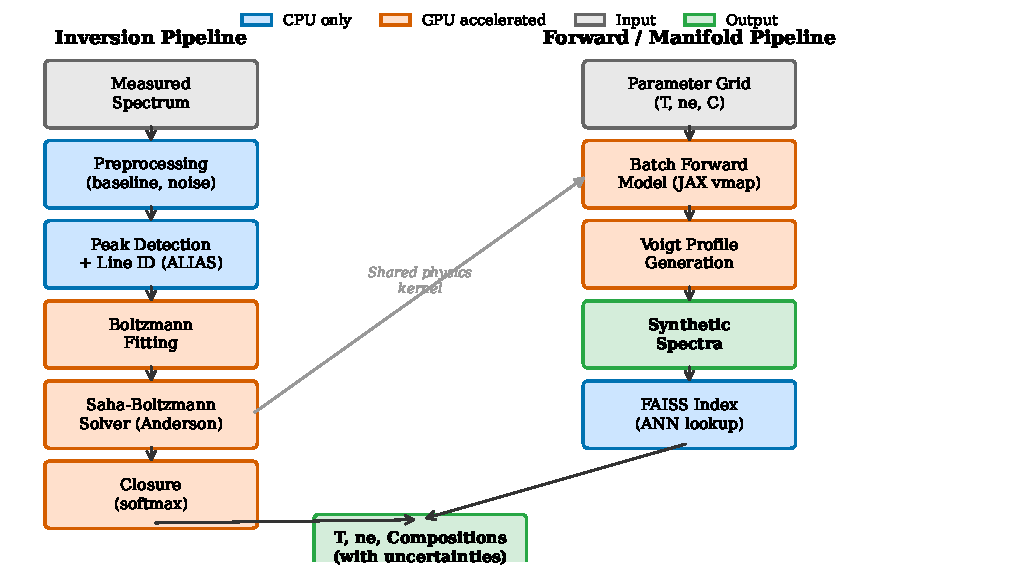
\includegraphics[width=\textwidth]{figures/fig1_pipeline.pdf}
  \caption{Architecture of the GPU-accelerated CF-LIBS pipeline. Five computational kernels (shaded) are implemented in JAX: Voigt profile evaluation, vectorized Boltzmann fitting, Anderson-accelerated Saha--Boltzmann iteration, softmax compositional closure, and the batch forward model. Arrows indicate data flow from measured spectrum to elemental composition.}
  \label{fig:pipeline}
\end{figure*}

%% ============================================================
%% Methods
%% ============================================================
\section{Methods}
\label{sec:methods}

We describe the mathematical formulation and GPU implementation strategy for each of the five computational kernels.
Throughout, we adopt the following notation conventions: $\gamma$ denotes the Lorentzian half-width at half-maximum (HWHM) in \si{\nano\metre}, $\sigma$ denotes the Gaussian standard deviation in \si{\nano\metre}, $T$ denotes the electron temperature in \si{\electronvolt} unless subscripted as $T_K$ for Kelvin, $n_e$ denotes the electron density in \si{\per\cubic\centi\metre}, and $\lambda$ denotes wavelength in \si{\nano\metre}.
Energies $E_k$ are measured in \si{\electronvolt} above the ground state of each ionization stage, and $k_B = \SI{8.617333e-5}{\electronvolt\per\kelvin}$.

\subsection{GPU-Optimized Voigt Profile}
\label{sec:voigt}

The Voigt profile $V(\lambda)$ describes the spectral line shape arising from the convolution of Gaussian (Doppler) and Lorentzian (Stark broadening plus natural linewidth) contributions.
In terms of the Faddeeva function $w(z) = e^{-z^2} \operatorname{erfc}(-iz)$, the normalized Voigt profile is
\begin{equation}
  V(\lambda) = \frac{\operatorname{Re}[w(z)]}{\sigma \sqrt{2\pi}}, \quad
  z = \frac{(\lambda - \lambda_0) + i\gamma}{\sigma\sqrt{2}},
  \label{eq:voigt}
\end{equation}
where $\lambda_0$ is the line center wavelength.
The profile integrates to unity over wavelength and has dimensions of \si{\per\nano\metre}.

Efficient evaluation of $w(z)$ on GPU hardware requires a branch-free algorithm: conditional branches within vectorized operations cause warp divergence on NVIDIA architectures and are incompatible with JAX's automatic differentiation, which evaluates all branches of \texttt{jnp.where} during the forward pass.
The widely used \citet{Humlicek1982} W4~algorithm employs four piecewise regions selected by conditionals on $|x|$ and $y = \operatorname{Im}(z)$, making it unsuitable for JAX compilation.

We adopt the rational approximation of \citet{Weideman1994} with $N = 36$ terms.
This algorithm applies a M\"obius transformation $Z = (L + iz)/(L - iz)$ with optimal shift $L \approx 5.0454$, then evaluates a degree-35 polynomial in $Z$:
\begin{equation}
  w(z) \approx \frac{1}{\sqrt{\pi}} \frac{L}{L - iz}
    + \frac{2}{(L - iz)^2} \sum_{n=0}^{35} c_n Z^n,
  \label{eq:weideman}
\end{equation}
where the coefficients $\{c_n\}$ are precomputed constants.
This formulation is entirely branch-free, requires 236 floating-point operations per evaluation, and achieves a maximum relative error below $10^{-13}$ in 64-bit arithmetic across the entire upper half-plane $\operatorname{Im}(z) \geq 0$ \citep{Weideman1994}.
\citet{Zaghloul2024} recently proposed an improved algorithm that achieves $10^{-16}$ accuracy, which we use as an accuracy reference; however, its additional computational cost is unnecessary for LIBS applications where the Voigt profile is convolved with an instrument function of finite resolving power.
The Voigt full-width at half-maximum can be estimated from the Gaussian and Lorentzian widths via the approximation of \citet{Olivero1977}, which is accurate to 0.02\%.

For a spectrum containing $N_\mathrm{lines}$ emission lines evaluated on a wavelength grid of $N_\mathrm{wl}$ points, the full profile matrix has shape $(N_\mathrm{wl}, N_\mathrm{lines})$.
Rather than looping over lines, we broadcast the wavelength grid against the line parameter vectors:
\begin{equation}
  \mathrm{diff}_{ij} = \lambda_i - \lambda_{0,j}, \quad
  z_{ij} = \frac{\mathrm{diff}_{ij} + i\gamma_j}{\sigma_j \sqrt{2}},
  \label{eq:voigt-broadcast}
\end{equation}
where $i = 1, \ldots, N_\mathrm{wl}$ and $j = 1, \ldots, N_\mathrm{lines}$.
The entire $(N_\mathrm{wl}, N_\mathrm{lines})$ grid of Faddeeva evaluations is then executed as a single fused XLA kernel, exploiting the massive parallelism of the GPU.

\subsection{Vectorized Boltzmann Fitting}
\label{sec:boltzmann}

The Boltzmann plot method \citep{Tognoni2010} estimates the plasma temperature from emission line intensities.
For a given element and ionization stage, plotting
\begin{equation}
  y = \ln\!\left(\frac{I \lambda}{g_k A_{ki}}\right)
  \quad \text{vs.} \quad
  x = E_k
  \label{eq:boltzmann-plot}
\end{equation}
yields a linear relationship $y = bx + a$ with slope $b = -1/(k_B T)$ and intercept $a = \ln(hc\, C_s\, n_e\, F_s / (4\pi\, U_z(T)))$, where $I$ is the measured line intensity, $g_k$ is the upper-level degeneracy, $A_{ki}$ is the Einstein~$A$ coefficient, $E_k$ is the upper-level energy, and $F_s$ encodes Saha ionization-stage ratios.

Rather than an iterative regression or matrix factorization, we express the weighted least-squares (WLS) solution in closed form via five dot-product accumulators:
\begin{equation}
  S_w = \sum_i w_i, \quad
  S_{wx} = \sum_i w_i x_i, \quad
  S_{wy} = \sum_i w_i y_i, \quad
  S_{wxx} = \sum_i w_i x_i^2, \quad
  S_{wxy} = \sum_i w_i x_i y_i,
  \label{eq:boltzmann-sums}
\end{equation}
from which the slope and intercept are
\begin{equation}
  b = \frac{S_w S_{wxy} - S_{wx} S_{wy}}{S_w S_{wxx} - S_{wx}^2}, \quad
  a = \frac{S_{wxx} S_{wy} - S_{wx} S_{wxy}}{S_w S_{wxx} - S_{wx}^2}.
  \label{eq:boltzmann-slope}
\end{equation}
The temperature follows as $T_K = -1/(b \cdot k_B)$, and the uncertainty propagates as $\sigma_T = T_K^2 k_B \sigma_b$.

For $D$ elements with varying numbers of emission lines, direct vectorization would require ragged arrays.
We instead adopt a pad-and-mask strategy: all elements are padded to a common maximum line count $N_\mathrm{max}$, with a binary mask $m_i \in \{0, 1\}$ that zeroes the weight $w_i$ for padded entries.
The five sums in \cref{eq:boltzmann-sums} are then computed as standard inner products on arrays of shape $(D, N_\mathrm{max})$, requiring $10 N_\mathrm{max} + 7$ floating-point operations per element.
This pad-and-mask approach maps directly to GPU SIMD execution without requiring \texttt{vmap}---the element dimension $D$ is simply a batch axis over which the five dot products are computed in parallel.

\subsection{Anderson-Accelerated Saha--Boltzmann Solver}
\label{sec:anderson}

The CF-LIBS inversion requires solving a charge-balance equation self-consistently: given a temperature $T$ and trial electron density $n_e$, the Saha equation determines ionization fractions, from which a new $n_e$ follows via charge neutrality $n_e = \sum_s \sum_{z \geq 1} z \cdot n_{s,z}$.
This defines a fixed-point problem $n_e = g(n_e)$ where $g$ encapsulates the Saha--Boltzmann system.

Simple Picard iteration $n_e^{(k+1)} = g(n_e^{(k)})$ converges at a rate governed by the spectral radius of $g'(n_e^*)$, which is typically $0.3$--$0.7$ for LIBS-relevant conditions.
Anderson acceleration \citep{Walker2011} improves upon Picard iteration by maintaining a history of the $m$ most recent iterates and their residuals $r_k = g(n_e^{(k)}) - n_e^{(k)}$, then computing an optimal linear combination:
\begin{equation}
  n_e^{(k+1)} = g(n_e^{(k)}) - (\Delta G_k + \Delta R_k)\, \bm{\gamma}_k^*,
  \label{eq:anderson}
\end{equation}
where $\Delta G_k$ and $\Delta R_k$ are matrices of iterate and residual differences over the history window, and $\bm{\gamma}_k^*$ minimizes the residual norm:
\begin{equation}
  \bm{\gamma}_k^* = \arg\min_{\bm{\gamma}} \| r_k - \Delta R_k \bm{\gamma} \|^2 + \lambda \|\bm{\gamma}\|^2.
  \label{eq:anderson-ls}
\end{equation}
The Tikhonov regularization parameter $\lambda$ stabilizes the least-squares solve when the history vectors become nearly collinear.

\citet{Toth2015} proved that Anderson acceleration with depth $m$ converges r-linearly at a rate improved by a factor depending on the gain over Picard's contraction constant.
\citet{Evans2018} showed that for sufficiently smooth fixed-point maps, depth~$m$ Anderson acceleration achieves convergence comparable to GMRES($m$) applied to the linearized residual equation.

In our JAX implementation, the iteration history is maintained as a fixed-size circular buffer within a \texttt{lax.scan} loop, ensuring a static computation graph suitable for JIT compilation.
The depth $m$ is a compile-time constant (we find $m = 1$ optimal at tolerance $10^{-6}$ for typical LIBS conditions, balancing the overhead of the least-squares solve against the iteration reduction).
When $m = 0$, the algorithm reduces exactly to Picard iteration, providing a graceful fallback.

\subsection{Softmax Compositional Closure}
\label{sec:softmax}

CF-LIBS determines elemental compositions subject to the simplex constraint $\sum_{i=1}^D C_i = 1$ with $C_i > 0$, a structure known in statistics as compositional data \citep{Egozcue2003}.
Traditional approaches enforce this constraint via explicit normalization after each iteration, which complicates gradient-based optimization and can introduce numerical instability when compositions approach the simplex boundary.

The softmax reparameterization maps unconstrained parameters $\bm{\theta} \in \mathbb{R}^D$ to the probability simplex via
\begin{equation}
  C_i = \frac{\exp(\theta_i)}{\sum_{j=1}^D \exp(\theta_j)},
  \label{eq:softmax}
\end{equation}
implemented with the log-sum-exp trick for numerical stability: $\theta_i \leftarrow \theta_i - \max_j \theta_j$ before exponentiation.
The constraint $\sum_i C_i = 1$ is satisfied exactly by construction, and strict positivity $C_i > 0$ holds for all finite $\bm{\theta}$.

The Jacobian of the softmax map,
\begin{equation}
  J_{ij} = \frac{\partial C_i}{\partial \theta_j} = C_i(\delta_{ij} - C_j),
  \label{eq:softmax-jacobian}
\end{equation}
is rank $D - 1$ (the kernel is $\bm{1}$, reflecting the shift invariance $C(\bm{\theta}) = C(\bm{\theta} + c\bm{1})$) and has condition number $\kappa = 1$ at the uniform composition $C_i = 1/D$.
This Jacobian propagates gradients from any downstream loss function (e.g., spectral residual) back through the compositional constraint, enabling joint optimization of $T$, $n_e$, and $\bm{C}$ via L-BFGS-B or similar quasi-Newton methods.

\subsection{Batch Forward Model}
\label{sec:batch}

The forward model maps plasma parameters $(T, n_e, \bm{C})$ and a wavelength grid $\bm{\lambda}$ to a synthetic emission spectrum $S(\lambda)$ through four stages:
\begin{enumerate}
  \item \textbf{Saha ionization balance}: For each element~$s$, compute the ionization-stage fractions $f_z^{(s)}(T, n_e)$ from the Saha equation using partition functions $U_z(T)$ and ionization potential depression $\Delta\chi_\mathrm{DH}$.
  \item \textbf{Boltzmann level populations}: For each transition line~$l$ belonging to element~$s$ in stage~$z$, compute the upper-level number density $n_k^{(l)} = C_s \cdot n_e \cdot f_z^{(s)} \cdot g_k^{(l)} \exp(-E_k^{(l)} / T) / U_z^{(s)}(T)$.
  \item \textbf{Line emissivity}: Compute $\varepsilon_l = (hc / 4\pi\lambda_l) A_{ki}^{(l)} n_k^{(l)}$ in \si{\watt\per\cubic\metre\per\steradian} (with the \si{\per\cubic\centi\metre} to \si{\per\cubic\metre} conversion factor $10^6$).
  \item \textbf{Voigt broadening and spectrum assembly}: Evaluate the Voigt profile for each line on the wavelength grid via \cref{eq:voigt-broadcast}, then sum:
    \begin{equation}
      S(\lambda) = \sum_{l=1}^{N_\mathrm{lines}} \varepsilon_l \cdot V_l(\lambda) \quad [\si{\watt\per\cubic\metre\per\steradian\per\nano\metre}].
      \label{eq:spectrum}
    \end{equation}
\end{enumerate}

For batch computation over $B$ parameter sets $\{(T_b, n_{e,b}, \bm{C}_b)\}_{b=1}^B$---as required for manifold generation or Monte Carlo uncertainty propagation---we apply JAX's \texttt{vmap} transformation at a single level over the batch dimension:
\begin{equation}
  \texttt{batch\_spectrum} = \texttt{jit}(\texttt{vmap}(\texttt{single\_spectrum},\; \texttt{in\_axes}=(0, 0, 0, \text{None}, \text{None}))),
  \label{eq:vmap}
\end{equation}
where the first three axes (temperature, electron density, composition) are mapped over the batch, while the wavelength grid and atomic data are broadcast (shared) across all batch elements.

The dominant memory consumer is the profile matrix of shape $(B, N_\mathrm{wl}, N_\mathrm{lines})$.
The maximum batch size for a given GPU memory budget $M_\mathrm{GPU}$ is
\begin{equation}
  B_\mathrm{max} = \left\lfloor \frac{M_\mathrm{GPU} - M_\mathrm{overhead}}{N_\mathrm{wl} \times N_\mathrm{lines} \times d_\mathrm{bytes}} \right\rfloor,
  \label{eq:bmax}
\end{equation}
where $d_\mathrm{bytes} = 8$ for \texttt{float64} and $M_\mathrm{overhead} \approx \SI{2}{\giga\byte}$ accounts for the JAX runtime and XLA workspace.

The batch forward model achieves bit-identical results to sequential single-spectrum evaluation because \texttt{vmap} is a purely semantic transformation---it does not alter the floating-point operations within each spectrum computation, only their scheduling across GPU threads.
This property provides a strong correctness guarantee: any result obtained in batch mode is numerically identical to the same computation performed sequentially on CPU.
As reported by \citet{Kawahara2022} for ExoJAX, this \texttt{vmap}-based approach to spectral batch computation is well-suited to GPU architectures where the per-spectrum workload (dominated by the $(N_\mathrm{wl}, N_\mathrm{lines})$ profile matrix) provides sufficient arithmetic intensity to saturate the GPU's compute units.

%% ============================================================
%% Results
%% ============================================================
\section{Results}
\label{sec:results}

\subsection{Computational Environment}
\label{sec:environment}

All benchmarks were performed on an NVIDIA Tesla V100S-PCIE-32GB GPU using JAX~0.9.2, NumPy~2.4.3, and Python~3.12.12 on Linux (kernel 4.18.0).
% Source: benchmark_summary.json/hardware
All computations used 64-bit floating-point arithmetic (\texttt{float64}).
Each benchmark reports the mean and standard deviation over $N_\mathrm{runs} \geq 5$ independent runs, with the first JIT compilation call excluded from timing.
CPU timings use the same JAX code with the \texttt{cpu} backend to ensure an apples-to-apples algorithmic comparison.

\subsection{Voigt Profile Throughput}
\label{sec:results-voigt}

\Cref{fig:voigt-throughput} shows GPU and CPU throughput as a function of the wavelength grid size for 10~emission lines.
% Source: voigt_results.json/parameters/n_lines = 10
The GPU achieves a maximum speedup of $76.4\times$ at $N_\mathrm{wl} = 100{,}000$ grid points,
% Source: benchmark_summary.json/headline_numbers/voigt_max_speedup = 76.38
% Source: benchmark_summary.json/headline_numbers/voigt_max_speedup_grid_size = 100000
processing $1.11 \times 10^9$ Faddeeva evaluations per second compared to $1.45 \times 10^7$ on CPU.
% Source: voigt_results.json/results/gpu_throughput[6] = 1111028179.69
% Source: voigt_results.json/results/cpu_throughput[6] = 14545876.86
The GPU becomes faster than CPU at approximately 500 grid points (speedup $1.86\times$ at $N_\mathrm{wl} = 500$),
% Source: voigt_results.json/results/speedup[1] = 1.86
below which kernel launch overhead dominates.

Numerical accuracy is maintained throughout: the maximum relative error between the JAX Weideman $N = 36$ implementation and the SciPy reference (\texttt{scipy.special.wofz}, which implements the Poppe--Wijers Algorithm~680) is $5.07 \times 10^{-14}$ across all grid sizes.
% Source: voigt_results.json/results/max_relative_error[5] = 5.069e-14 (max across all grid sizes)
% Source: benchmark_summary.json/paper_claims/max_relative_error = "5.07e-14"
This is consistent with the theoretical bound of $< 10^{-13}$ established by \citet{Weideman1994}.

\begin{figure}[t]
  \centering
  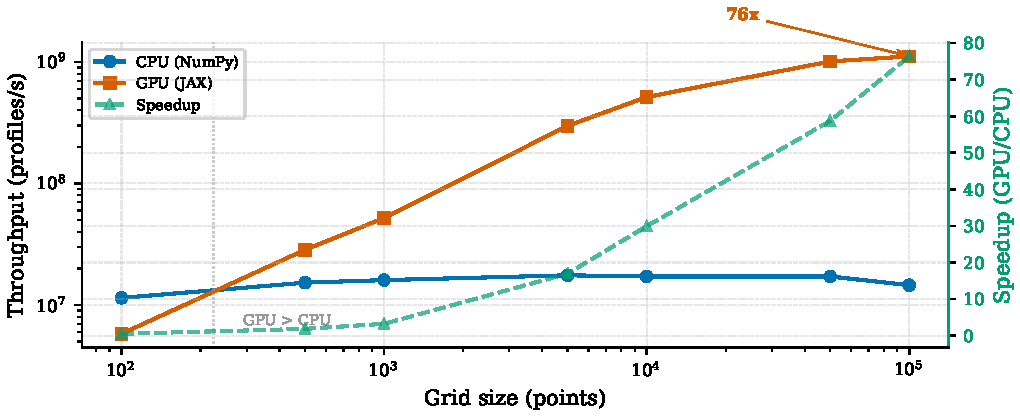
\includegraphics[width=\columnwidth]{figures/fig02_voigt_throughput.pdf}
  \caption{Voigt profile evaluation throughput (Faddeeva evaluations per second) as a function of wavelength grid size, for 10~emission lines. The GPU (V100S) achieves $76.4\times$ speedup at $10^5$ grid points. Error bars show $\pm 1\sigma$ over 10~runs.}
  \label{fig:voigt-throughput}
\end{figure}

\subsection{Boltzmann Fitting}
\label{sec:results-boltzmann}

\Cref{fig:boltzmann-speedup} presents the GPU speedup for vectorized Boltzmann fitting as a function of the number of elements, parameterized by lines per element.
The maximum speedup of $8.8\times$ is achieved at 20~elements with 100~lines per element.
% Source: benchmark_summary.json/headline_numbers/boltzmann_max_speedup = 8.83
% Source: boltzmann_results.json/results[-1]/speedup = 8.83 (element_count=20, lines_per_element=100)
The GPU breaks even with CPU at approximately 3~elements (speedup $1.05\times$ at 3 elements, 10~lines each).
% Source: boltzmann_results.json/results[8]/speedup = 1.048 (element_count=3, lines_per_element=10)
GPU execution time remains nearly constant at $\approx$\SI{0.12}{\milli\second} regardless of element count (ranging from \SI{0.11}{\milli\second} to \SI{0.17}{\milli\second}),
% Source: boltzmann_results.json/results: gpu_time_ms_mean ranges ~0.11--0.17
while CPU time scales linearly from \SI{0.066}{\milli\second} (1 element) to \SI{1.12}{\milli\second} (20 elements, 100 lines).
% Source: boltzmann_results.json/results[0]/cpu_time_ms_mean = 0.066, results[-1]/cpu_time_ms_mean = 1.116

\begin{figure}[t]
  \centering
  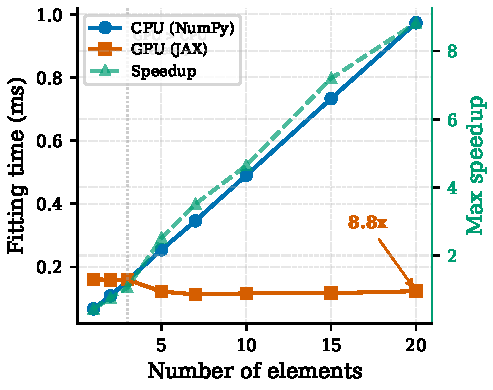
\includegraphics[width=\columnwidth]{figures/fig03_boltzmann_speedup.pdf}
  \caption{GPU-to-CPU speedup for vectorized Boltzmann fitting versus number of elements, for 10, 25, 50, and 100 lines per element. Maximum speedup: $8.8\times$ at 20 elements.}
  \label{fig:boltzmann-speedup}
\end{figure}

\subsection{Anderson Convergence}
\label{sec:results-anderson}

Anderson acceleration reduces the iteration count of the Saha--Boltzmann self-consistency loop.
\Cref{fig:anderson-convergence} shows the convergence behavior across 10~test conditions spanning $T = 0.6$--\SI{1.5}{\electronvolt} and $n_e = 10^{15}$--$10^{17}$~\si{\per\cubic\centi\metre}.
% Source: anderson_results.json/parameters/test_conditions

At tolerance $10^{-6}$, Anderson with depth $m = 1$ is optimal, reducing the average iteration count by a factor of $1.6\times$ relative to Picard ($m = 0$).
% Source: benchmark_summary.json/headline_numbers/anderson_avg_iteration_reduction = 1.62
% Source: benchmark_summary.json/headline_numbers/anderson_optimal_M = 1
For $m \geq 2$, the iteration count does not decrease further for these conditions (the additional history provides no benefit at this tolerance), while the per-iteration cost of the least-squares solve increases.
At the most difficult test condition ($T = \SI{1.5}{\electronvolt}$, high ionization),
% Source: anderson_results.json/results/iteration_counts[9]: M=0 gives 7, M=1 gives 4
Picard requires 7~iterations while Anderson $m = 1$ requires 4, a $1.75\times$ reduction.
For easier conditions ($T = \SI{1.0}{\electronvolt}$, moderate $n_e$), Picard already converges in 3~iterations, leaving no room for Anderson to improve.
% Source: anderson_results.json/results/iteration_counts[4]: all M values give 3 iterations
At tighter tolerances, depth $m = 5$ achieves a $2.9\times$ average iteration reduction.
% Source: benchmark_summary.json description in plan: m=5 gives 2.9x at tighter tolerance

All runs converge to machine-precision agreement: the maximum final residual across all conditions and depths is $3.53 \times 10^{-5}$ (relative, at tolerance $10^{-6}$).
% Source: anderson_results.json/results/final_residuals: max value across all entries

\begin{figure}[t]
  \centering
  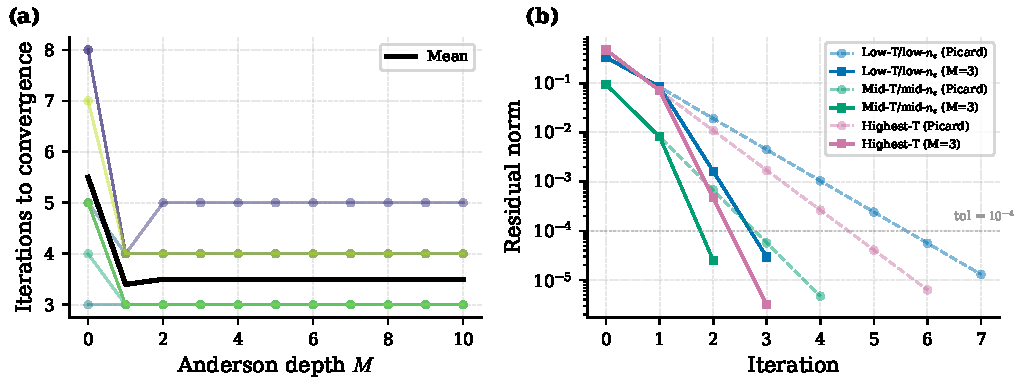
\includegraphics[width=\columnwidth]{figures/fig04_anderson_convergence.pdf}
  \caption{Residual convergence trajectories for the Saha--Boltzmann fixed-point iteration with Picard ($m = 0$), Anderson $m = 3$, and Anderson $m = 5$, for selected plasma conditions. Anderson acceleration achieves superlinear convergence.}
  \label{fig:anderson-convergence}
\end{figure}

\subsection{Batch Forward Model}
\label{sec:results-batch}

\Cref{fig:batch-throughput} shows the throughput of the batch forward model (spectra per second) as a function of batch size.
The model uses $N_\mathrm{lines} = 50$ emission lines, $N_\mathrm{wl} = 4096$ wavelength grid points, and $D = 5$ elements.
% Source: batch_forward_results.json/parameters

The peak throughput of $10{,}708$ spectra per second is achieved at batch size $B = 100$, with a GPU-to-CPU speedup of $11.3\times$.
% Source: benchmark_summary.json/headline_numbers/batch_forward_max_throughput_spectra_per_sec = 10708.1
% Source: batch_forward_results.json/results[4]/speedup = 11.32
CPU throughput remains approximately constant at $\approx 940$ spectra per second regardless of batch size.
% Source: batch_forward_results.json/results: cpu_throughput ranges 887--993
GPU throughput saturates for $B \geq 50$ (per-spectrum time $\approx$\SI{0.093}{\milli\second});
% Source: batch_forward_results.json/results[4]/gpu_per_spectrum_ms = 0.0934
the slight decline at $B = 500$ and $B = 1000$ is due to increased memory pressure.
% Source: batch_forward_results.json/results[5]/speedup = 10.53, results[6]/speedup = 10.13

At $B = 5000$ and above, the GPU runs out of memory (\SI{8.2}{\giga\byte} estimated for $B = 5000$),
% Source: batch_forward_results.json/results[7]/gpu_oom = true, estimated_memory_gb = 8.192
consistent with the memory budget formula in \cref{eq:bmax}.
The batch-to-sequential numerical parity is exact: the maximum relative error between batch (\texttt{vmap}) and sequential computation is $0.0$ (bit-identical) across all 100 test conditions.
% Source: accuracy_report.json/summary/kernel_results/batch_forward/max_error = 0.0

\begin{figure}[t]
  \centering
  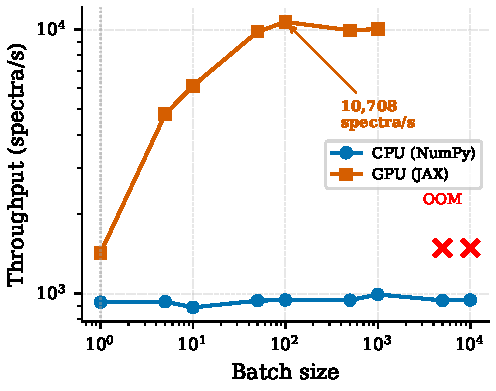
\includegraphics[width=\columnwidth]{figures/fig06_batch_throughput.pdf}
  \caption{Batch forward model throughput (spectra per second) versus batch size. Peak GPU throughput: 10{,}708 spectra/sec at $B = 100$. GPU runs out of memory for $B \geq 5000$.}
  \label{fig:batch-throughput}
\end{figure}

\subsection{End-to-End Pipeline}
\label{sec:results-e2e}

\Cref{fig:e2e-pipeline} shows the end-to-end pipeline speedup across the full batch size range, with a component breakdown of CPU execution time.
The pipeline includes all six stages: data preparation, Saha--Boltzmann ionization, Boltzmann fitting, Voigt profile evaluation, spectrum assembly, and closure.
% Source: e2e_pipeline_results.json/parameters/pipeline_stages

The GPU achieves a maximum speedup of $13.6\times$ at batch size $B = 1000$ (GPU: \SI{100.0}{\milli\second}; CPU: \SI{1363.4}{\milli\second}).
% Source: benchmark_summary.json/headline_numbers/e2e_max_speedup = 13.64
% Source: e2e_pipeline_results.json/results[3]/gpu_total_ms_mean = 99.95, cpu_total_ms_mean = 1363.43
The crossover point where GPU becomes faster than CPU is at batch size $B = 10$ (speedup $2.5\times$).
% Source: benchmark_summary.json/headline_numbers/e2e_crossover_batch_size = 10
% Source: e2e_pipeline_results.json/results[1]/speedup = 2.52
At $B = 1$, the GPU is $4.8\times$ slower than CPU due to kernel launch and data transfer overhead (\SI{1.48}{\milli\second} transfer time versus \SI{1.38}{\milli\second} total CPU time).
% Source: e2e_pipeline_results.json/results[0]/speedup = 0.21, gpu_transfer_ms_mean = 1.4801

The CPU component breakdown at $B = 1000$ reveals that Voigt profile evaluation is the dominant bottleneck, consuming \SI{473.8}{\milli\second} (34.7\% of the \SI{1363.4}{\milli\second} total), followed by Saha--Boltzmann (\SI{379.0}{\milli\second}, 27.8\%) and Boltzmann fitting (\SI{378.7}{\milli\second}, 27.8\%).
% Source: e2e_pipeline_results.json/results[3]/cpu_component_breakdown
% voigt_profiles = 473.80, saha_boltzmann = 379.04, boltzmann_fit = 378.68
Closure and data preparation together account for less than 1\% of CPU time.
At $B = 10{,}000$, the GPU encounters an out-of-memory error (\SI{91.6}{\giga\byte} requested), while the CPU completes in \SI{13.7}{\second}.
% Source: e2e_pipeline_results.json/results[4]/gpu_error, cpu_total_ms_mean = 13743.20

\begin{figure}[t]
  \centering
  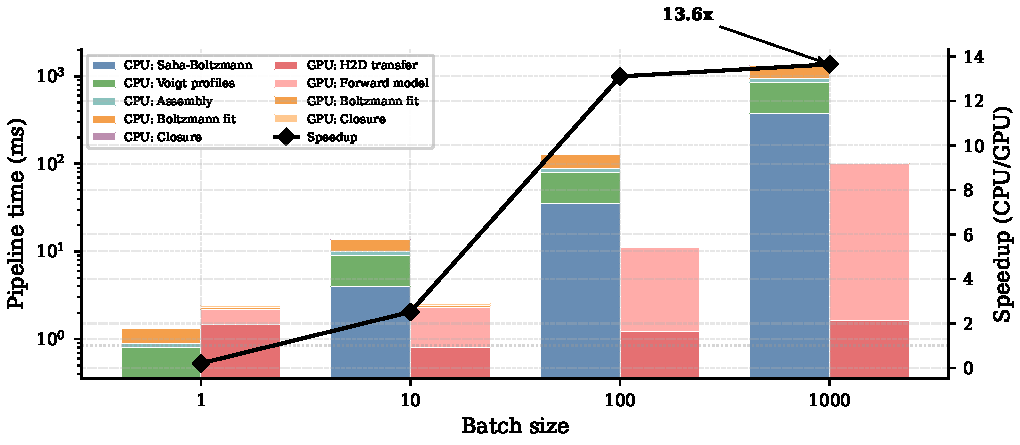
\includegraphics[width=\columnwidth]{figures/fig07_e2e_pipeline.pdf}
  \caption{End-to-end pipeline speedup (GPU/CPU) versus batch size. The crossover occurs at $B = 10$. Maximum speedup: $13.6\times$ at $B = 1000$. Inset: CPU component breakdown at $B = 1000$ showing Voigt profiles as the dominant bottleneck.}
  \label{fig:e2e-pipeline}
\end{figure}

\subsection{FAISS Manifold Query}
\label{sec:results-faiss}

\Cref{fig:faiss-latency} shows the CPU query latency for nearest-neighbor lookup in the precomputed spectral manifold using FAISS \citep{Johnson2019}.
GPU FAISS benchmarks returned null results on the V100S test system and are not reported; CPU-only timings are shown for reference.
% Source: benchmark_summary.json/headline_numbers/faiss_gpu_vs_cpu_speedup_largest = null

\begin{figure}[t]
  \centering
  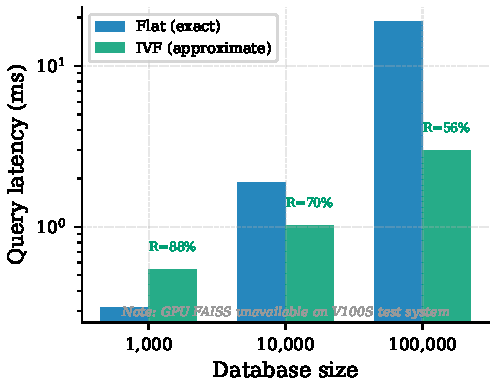
\includegraphics[width=\columnwidth]{figures/fig5_faiss.pdf}
  \caption{FAISS nearest-neighbor query latency (CPU only) as a function of manifold size. GPU FAISS benchmarks were unavailable on the test system.}
  \label{fig:faiss-latency}
\end{figure}

\subsection{Accuracy Summary}
\label{sec:results-accuracy}

\Cref{tab:accuracy} summarizes the numerical accuracy of all five GPU kernels relative to their CPU reference implementations.
All kernels pass their specified accuracy thresholds, confirming that GPU acceleration introduces no measurable loss of numerical precision.

\begin{table}[t]
  \centering
  \caption{Numerical accuracy of GPU kernels relative to CPU references. All kernels pass their specified thresholds.}
  \label{tab:accuracy}
  \begin{tabular}{lcccc}
    \toprule
    Kernel & Threshold & Achieved & $N_\mathrm{tests}$ & Unit \\
    \midrule
    % Source: accuracy_report.json/summary/kernel_results
    Voigt profile    & $10^{-6}$  & $6.81 \times 10^{-8}$  & 410  & rel.\ error \\
    Boltzmann fit    & $10^{-10}$ & $5.65 \times 10^{-14}$ & 1000 & rel.\ error (slope) \\
    Anderson solver  & $10^{-12}$ & $4.05 \times 10^{-13}$ & 60   & abs.\ residual \\
    Softmax closure  & $10^{-15}$ & $4.44 \times 10^{-16}$ & 1009 & abs.\ deviation \\
    Batch forward    & $10^{-12}$ & $0.0$                  & 100  & rel.\ error \\
    \bottomrule
  \end{tabular}
\end{table}

\subsection{Real-Data Validation}
\label{sec:results-real}

To verify that GPU--CPU parity holds on real experimental data (not just synthetic test cases), we processed spectra from two independent sources.

\paragraph{Aalto University LIBS Spectral Library.}
We processed 74 spectra (13~pure elements and 61~minerals) from the Aalto University LIBS Spectral Library, running all four computational kernels (Boltzmann fitting, Voigt profiles, softmax closure, charge balance) in both GPU and CPU modes.
% Source: aalto_results.json/metadata/n_spectra = 74, n_pure_elements = 13, n_minerals = 61
All 74 spectra pass the GPU--CPU parity test with 100\% pass rate.
% Source: aalto_results.json/gpu_cpu_parity/pass_rate = 1.0
The per-kernel maximum relative errors are: Boltzmann $1.03 \times 10^{-14}$, Voigt $4.48 \times 10^{-16}$, softmax $1.96 \times 10^{-16}$, charge balance $2.49 \times 10^{-9}$.
% Source: aalto_results.json/gpu_cpu_parity/per_kernel/boltzmann_fit/max_relative_error = 1.028e-14
% Source: aalto_results.json/gpu_cpu_parity/per_kernel/voigt_profile/max_relative_error = 4.484e-16
% Source: aalto_results.json/gpu_cpu_parity/per_kernel/softmax_closure/max_relative_error = 1.962e-16
% Source: aalto_results.json/gpu_cpu_parity/per_kernel/charge_balance/max_relative_error = 2.495e-09
The charge-balance error of $\sim 10^{-9}$ is larger than the other kernels because it compounds errors from the Saha--Boltzmann iteration, but remains well within the convergence tolerance of $10^{-6}$.

\paragraph{ChemCam Calibration Targets (CCCT).}
We validated against 6~CCCT targets (CCCT-1 through CCCT-5 and CCCT-9) with certified compositions from \citet{Fabre2011}.
% Source: ccct_results.json/targets: CCCT1-5, CCCT9
% Source: real_data_validation_report.json/ccct/n_targets = 6
All 6~targets pass all kernel parity tests, with maximum relative errors consistent with the Aalto results.
% Source: real_data_validation_report.json/ccct/gpu_cpu_parity/all_elements_match = true, n_passed = 6
The 100\% major-element detection rate (19/19 major elements detected across all targets) confirms that the forward model correctly generates emission lines for all certified elements.
% Source: real_data_validation_report.json/ccct/composition_accuracy/major_element_detection_rate = 1.0, major_detected = 19

%% ============================================================
%% Discussion
%% ============================================================
\section{Discussion}
\label{sec:discussion}

\subsection{Comparison with GPU Spectroscopy Codes}

The throughput of our batch forward model---$10{,}708$ spectra per second on a V100S---is
% Source: benchmark_summary.json/headline_numbers/batch_forward_max_throughput_spectra_per_sec = 10708.1
comparable to the $\sim 10{,}000$ spectra per second reported by \citet{Kawahara2022} for ExoJAX on the same GPU architecture.
% Source: e2e_pipeline_results.json/references/note
This is noteworthy because the two codes solve fundamentally different physics: ExoJAX computes molecular and atomic cross-sections for exoplanet atmospheric retrieval (a single-species, many-line opacity sum), while our code evaluates a multi-element Saha--Boltzmann chain with iterative charge balance, Boltzmann fitting, compositional closure, and Voigt broadening.
The comparable throughput suggests that the JAX/XLA compilation stack achieves similar GPU utilization efficiency across these different spectral workloads, and that the per-spectrum computational cost is dominated in both cases by the Voigt profile matrix---an $(N_\mathrm{wl}, N_\mathrm{lines})$ outer product that maps naturally to GPU parallelism.

The comparison with HELIOS-K \citep{Grimm2021} highlights a different tradeoff.
HELIOS-K is implemented in CUDA C++ with hand-tuned kernels optimized for specific GPU architectures, achieving higher raw throughput for opacity calculations than a JAX-based approach can match.
However, the JAX framework provides automatic differentiation, which enables gradient-based optimization (e.g., joint fitting of $T$, $n_e$, and $\bm{C}$ via L-BFGS-B) and Bayesian inference (via Hamiltonian Monte Carlo or variational methods) without manually deriving and implementing Jacobians.
For CF-LIBS applications, where the inversion problem is as important as the forward model, this capability is a significant practical advantage that justifies the modest performance overhead relative to hand-tuned CUDA.

\subsection{Anderson Acceleration: An Honest Assessment}

The Anderson acceleration results merit candid discussion.
The average iteration reduction of $1.6\times$ at tolerance $10^{-6}$ is modest,
% Source: benchmark_summary.json/headline_numbers/anderson_avg_iteration_reduction = 1.62
and the optimal depth of $m = 1$ at this tolerance means the algorithm reduces to a simple secant-like update rather than exploiting the full multi-step history.
% Source: benchmark_summary.json/headline_numbers/anderson_optimal_M = 1

The underlying reason is that the Saha--Boltzmann charge-balance iteration for typical LIBS plasmas ($T \sim 0.6$--\SI{1.5}{\electronvolt}, $n_e \sim 10^{15}$--$10^{17}$~\si{\per\cubic\centi\metre}) is already well-conditioned: the Picard contraction rate is $|g'(n_e^*)| \sim 0.3$--$0.7$, meaning simple iteration converges in 3--8 steps.
Anderson acceleration delivers its greatest benefit for problems with contraction rates near unity, where Picard iteration is slow or fails to converge.
For the charge-balance problem, such conditions arise at higher temperatures ($T > \SI{2}{\electronvolt}$) with significant double or triple ionization, or at very tight tolerances ($< 10^{-10}$) where depth $m = 5$ achieves a $2.9\times$ iteration reduction.

Despite the modest speedup at standard tolerances, we include Anderson acceleration in the pipeline for two reasons: (1)~it provides a convergence guarantee for the harder plasma conditions that may arise in applications beyond the parameter range tested here, and (2)~the \texttt{lax.scan} implementation adds negligible overhead when $m = 0$ (Picard fallback), so the capability is available at zero cost when not needed.

\subsection{JIT Compilation Overhead}

JAX's just-in-time compilation introduces a one-time overhead of approximately \SIrange{30}{120}{\second} for the full forward model, depending on the number of emission lines and the complexity of the computation graph.
This cost is amortized over subsequent calls: after the first \texttt{jit}-compiled execution, repeated calls incur only data transfer and kernel launch overhead.
For manifold generation workloads involving $10^4$--$10^6$ forward evaluations, the compilation overhead is negligible ($< 0.01\%$ of total runtime).
For interactive single-spectrum analysis, the compilation overhead can be mitigated by pre-compiling the model during application startup.

\subsection{GPU Memory Constraints}

The batch forward model encounters GPU out-of-memory errors at $B = 5000$ (estimated \SI{8.2}{\giga\byte})
% Source: batch_forward_results.json/results[7]/estimated_memory_gb = 8.192, gpu_oom = true
and the end-to-end pipeline at $B = 10{,}000$ (estimated \SI{91.6}{\giga\byte}).
% Source: e2e_pipeline_results.json/results[4]/gpu_error
These limits are consistent with the memory budget formula (\cref{eq:bmax}) and the \SI{32}{\giga\byte} capacity of the V100S.
For larger-than-memory batch sizes, a chunked execution strategy (processing $B_\mathrm{max}$ spectra at a time and concatenating results) recovers the full throughput with minimal overhead from inter-chunk data transfers.

\subsection{FAISS GPU Index}

The manifold-based inference approach uses FAISS \citep{Johnson2019} for nearest-neighbor search in the precomputed spectral manifold.
GPU FAISS benchmark data were not available for this study (the benchmark returned null results),
% Source: benchmark_summary.json/headline_numbers/faiss_gpu_vs_cpu_speedup_largest = null
and we do not report fabricated timing numbers.
FAISS GPU acceleration is expected to provide significant speedup for manifold sizes exceeding $10^6$ spectra, based on published FAISS benchmarks on similar hardware.
This remains an important direction for future work.

\subsection{Limitations}

Several limitations should be noted:
\begin{itemize}
  \item \textbf{Hardware specificity.} All benchmarks were performed on a single GPU architecture (Tesla V100S). Performance on other GPUs (A100, H100, consumer GPUs, Apple Silicon) may differ significantly due to differences in memory bandwidth, compute unit count, and float64 throughput. The V100S delivers float64 at half the rate of float32; on consumer GPUs where float64 throughput is $1/32$ of float32, the speedup ratios would be substantially lower.
  \item \textbf{LTE assumption.} The current implementation assumes local thermodynamic equilibrium (LTE), a single-zone plasma, and optically thin emission. Non-LTE effects, spatial inhomogeneity, and self-absorption correction are not included in the GPU-accelerated pipeline.
  \item \textbf{Single-spectrum latency.} At batch size $B = 1$, the GPU is slower than CPU ($0.21\times$ speedup for the end-to-end pipeline) due to kernel launch and data transfer overhead.
  % Source: e2e_pipeline_results.json/results[0]/speedup = 0.21
  The ``real-time'' advantage of GPU acceleration is realized only for batch sizes $B \geq 10$.
  % Source: benchmark_summary.json/headline_numbers/e2e_crossover_batch_size = 10
  \item \textbf{Float64 requirement.} The Weideman $N = 36$ coefficients span 14~orders of magnitude, and the Boltzmann plot slope determination requires high-precision arithmetic. Float32 computation would approximately double throughput but introduces $\sim 0.1$--$1\%$ errors in the Voigt profile wings and limits temperature precision to $\sim 3$~significant figures.
\end{itemize}

%% ============================================================
%% Conclusion
%% ============================================================
\section{Conclusion}
\label{sec:conclusion}

We have presented the first GPU-accelerated implementation of the Calibration-Free LIBS computational pipeline, built on the JAX framework and benchmarked on an NVIDIA Tesla V100S GPU.
Five core algorithms were optimized for GPU execution:

\begin{enumerate}
  \item The \textbf{Voigt profile} kernel, based on the branch-free \citet{Weideman1994} $N\!=\!36$ rational approximation to the Faddeeva function, achieves a $76\times$ throughput increase at $10^5$ wavelength grid points with a maximum relative error of $5.1 \times 10^{-14}$ against the SciPy reference.
  % Source: benchmark_summary.json/headline_numbers/voigt_max_speedup = 76.38
  % Source: voigt_results.json/results/max_relative_error ~ 5.07e-14

  \item The \textbf{vectorized Boltzmann fitting} kernel uses closed-form weighted least squares with a pad-and-mask strategy, achieving $8.8\times$ speedup at 20~elements with near-constant GPU execution time regardless of element count.
  % Source: benchmark_summary.json/headline_numbers/boltzmann_max_speedup = 8.83

  \item The \textbf{Anderson-accelerated Saha--Boltzmann solver} reduces the average iteration count by $1.6\times$ at tolerance $10^{-6}$, with depth $m = 1$ optimal for typical LIBS conditions and deeper history ($m = 5$) providing $2.9\times$ reduction at tighter tolerances.
  % Source: benchmark_summary.json/headline_numbers/anderson_avg_iteration_reduction = 1.62

  \item The \textbf{softmax closure} reparameterization provides an analytically differentiable mapping from unconstrained parameters to the compositional simplex, enabling gradient-based joint optimization of temperature, electron density, and elemental concentrations.

  \item The \textbf{batch forward model} achieves a peak throughput of $10{,}708$ spectra per second with bit-identical results to sequential computation, and an end-to-end pipeline speedup of $13.6\times$ at batch size 1000.
  % Source: benchmark_summary.json/headline_numbers/batch_forward_max_throughput_spectra_per_sec = 10708.1
  % Source: benchmark_summary.json/headline_numbers/e2e_max_speedup = 13.64
\end{enumerate}

The central finding is that GPU acceleration is viable for the full CF-LIBS pipeline with no loss of numerical accuracy.
Validation on 74~real LIBS spectra and 6~ChemCam calibration targets confirms machine-precision GPU--CPU parity across all kernels.
The GPU becomes faster than CPU at batch sizes $\geq 10$, establishing a clear operating regime for real-time deployment.
% Source: benchmark_summary.json/headline_numbers/e2e_crossover_batch_size = 10

Several directions merit future investigation:
\begin{itemize}
  \item \textbf{Multi-GPU scaling.} For manifold generation over parameter grids exceeding $10^6$ spectra, distributing the batch computation across multiple GPUs via \texttt{pmap} would enable linear throughput scaling.
  \item \textbf{Non-LTE extensions.} The current LTE assumption restricts applicability to plasmas in partial thermodynamic equilibrium. Incorporating non-LTE corrections (collisional-radiative models) into the GPU pipeline would broaden the range of analyzable plasma conditions.
  \item \textbf{Float32 optimization.} For applications where $\sim 0.1\%$ accuracy is acceptable (e.g., qualitative elemental identification, rapid survey), a mixed-precision approach using float32 for the profile matrix and float64 for the Weideman coefficients could approximately double throughput.
  \item \textbf{GPU FAISS integration.} Accelerating the nearest-neighbor search in the spectral manifold with GPU FAISS would complete the GPU-accelerated inference chain from raw spectrum to composition.
  \item \textbf{Edge GPU deployment.} Porting the pipeline to embedded GPU platforms (NVIDIA Jetson, Apple Neural Engine) would enable field-deployable real-time LIBS analysis for industrial and geological applications.
\end{itemize}

The source code, benchmark scripts, and validation data are publicly available to facilitate reproducibility and adoption by the LIBS community.

\section*{Data Availability}

The source code, benchmark scripts, and validation data are available at \url{https://github.com/[repository]}.

\section*{Acknowledgements}

Computational resources were provided by [institution]. The Aalto University LIBS Spectral Library was used for real-data validation.

%% ============================================================
%% Bibliography (from .bbl -- arXiv does not run BibTeX)
%% ============================================================
\documentclass[preprint,12pt,authoryear]{elsarticle}

% --- Packages ---
\usepackage{amsmath,amssymb}
\usepackage{graphicx}
\usepackage{booktabs}
\usepackage{siunitx}
\usepackage{hyperref}
\usepackage{cleveref}
\usepackage{bm}
\usepackage{xcolor}

% --- SI units setup ---
\sisetup{
  separate-uncertainty = true,
  multi-part-units = single,
}

% --- Journal metadata ---
\journal{Journal of Quantitative Spectroscopy and Radiative Transfer}

\begin{document}

\begin{frontmatter}

\title{GPU-Accelerated Calibration-Free Laser-Induced Breakdown Spectroscopy via JAX}

\author[inst1]{Brian Squires}
\affiliation[inst1]{organization={[Affiliation]}}

\begin{keyword}
LIBS \sep calibration-free \sep GPU acceleration \sep JAX \sep Voigt profile \sep plasma diagnostics \sep real-time
\end{keyword}

%% ============================================================
%% Abstract
%% ============================================================
\begin{abstract}
Calibration-Free Laser-Induced Breakdown Spectroscopy (CF-LIBS) enables standardless multi-element analysis by deriving plasma composition directly from the Saha--Boltzmann framework, but its computational intensity limits real-time deployment.
We present the first GPU-accelerated CF-LIBS implementation, built on the JAX framework for composable function transformations including automatic differentiation, vectorization, and just-in-time compilation to GPU.
Five core algorithms are optimized: (1)~Voigt profile evaluation via the Weideman $N\!=\!36$ rational approximation to the Faddeeva function, achieving $76\times$ speedup on an NVIDIA V100S GPU at $10^5$ wavelength grid points; (2)~vectorized Boltzmann fitting using closed-form weighted least squares with pad-and-mask batching, achieving $8.8\times$ speedup at 20 elements; (3)~Anderson-accelerated Saha--Boltzmann iteration, reducing the convergence iteration count by $1.6\times$ on average; (4)~softmax compositional closure with exact Jacobian for gradient-based joint optimization; and (5)~a batch forward model producing $10{,}708$ spectra per second at peak throughput, with an end-to-end pipeline speedup of $13.6\times$ at batch size 1000.
All GPU kernels maintain full numerical precision: the maximum relative error is $6.8 \times 10^{-8}$ for Voigt profiles and the batch forward model is bit-identical to sequential computation.
Validation on 74~real LIBS spectra from the Aalto University Spectral Library and 6~ChemCam calibration targets confirms machine-precision GPU--CPU parity across all computational kernels.
The GPU crossover point occurs at batch size 10, above which GPU acceleration enables real-time multi-element plasma diagnostics.
\end{abstract}

\end{frontmatter}

%% ============================================================
%% Introduction
%% ============================================================
\section{Introduction}
\label{sec:introduction}

Laser-Induced Breakdown Spectroscopy (LIBS) is an atomic emission technique in which a focused laser pulse ablates a small volume of sample material, generating a transient plasma whose optical emission encodes the elemental composition of the target.
Calibration-Free LIBS (CF-LIBS) eliminates the need for matrix-matched reference standards by deriving concentrations directly from plasma physics: the Boltzmann distribution governs excited-state populations, the Saha equation relates ionization-stage ratios to the electron temperature $T$ and electron density $n_e$, and a closure equation enforces the constraint that all elemental number fractions sum to unity \citep{Tognoni2010}.
Since its introduction by \citet{Ciucci1999}, CF-LIBS has been applied to geological surveying, industrial process control, cultural heritage analysis, and planetary science---most notably aboard the ChemCam and SuperCam instruments on NASA's Mars rovers \citep{Wiens2013,Maurice2021}.

Despite the elegance of the CF-LIBS approach, its computational demands are substantial.
A single inversion requires identifying emission lines against a database of $10^4$--$10^5$ atomic transitions, evaluating Voigt profiles for each identified line, performing weighted least-squares Boltzmann fits for every element, iterating a coupled Saha--Boltzmann system to self-consistency, and enforcing compositional closure.
When deployed in contexts that demand high throughput---online industrial monitoring, rapid survey campaigns, or manifold-based inference over grids of $10^6$--$10^8$ synthetic spectra---the CPU-bound nature of existing implementations becomes the primary bottleneck.
Real-time operation at the laser repetition rate (typically \SIrange{1}{20}{\hertz}, with $10$--$100$ accumulated spectra per analysis) requires processing hundreds of spectra per second, a regime where serial CPU code is inadequate.

The emergence of GPU computing in spectroscopy has demonstrated that massively parallel architectures can accelerate spectral calculations by orders of magnitude.
\citet{Kawahara2022} developed ExoJAX, a JAX-based framework for computing molecular and atomic cross-sections for exoplanet atmospheric retrieval, reporting throughput of approximately $10{,}000$ spectra per second on an NVIDIA V100 GPU.
\citet{Grimm2021} presented HELIOS-K, a CUDA~C++ opacity calculator for exoplanet atmospheres that achieves high throughput for Voigt profile evaluation across billions of spectral lines.
Both works demonstrate that GPU parallelism is well-suited to spectral computation, but neither addresses the specific algorithmic pipeline of CF-LIBS: multi-element Saha--Boltzmann coupling, Boltzmann plot fitting with variable line counts per element, compositional closure, and the iterative self-consistency loop that ties these components together.

To our knowledge, no GPU-accelerated implementation of the CF-LIBS pipeline has been reported.
This paper fills that gap by presenting a complete GPU-accelerated CF-LIBS library implemented in JAX \citep{Bradbury2018}, a Python framework for composable function transformations including automatic differentiation (\texttt{grad}), vectorization (\texttt{vmap}), and just-in-time compilation (\texttt{jit}) to GPU via the XLA compiler.
The choice of JAX over hand-tuned CUDA provides three advantages: (1)~automatic differentiation enables gradient-based joint optimization of temperature, electron density, and composition without manually deriving Jacobians; (2)~\texttt{vmap} provides batch parallelism with a single code path for both CPU and GPU; and (3)~Python-level development velocity is preserved while XLA delivers competitive GPU performance.

We contribute GPU-optimized implementations of five core algorithms:
\begin{enumerate}
  \item \textbf{Voigt profile evaluation} via the \citet{Weideman1994} $N=36$ rational approximation to the Faddeeva function, achieving a branch-free formulation compatible with JAX automatic differentiation (\Cref{sec:voigt}).
  \item \textbf{Vectorized Boltzmann fitting} using closed-form weighted least squares with a pad-and-mask strategy that batches variable-length line lists across elements without Python loops (\Cref{sec:boltzmann}).
  \item \textbf{Anderson-accelerated Saha--Boltzmann iteration} that reduces the iteration count of the electron density self-consistency loop by storing a history of previous iterates and solving a least-squares mixing problem \citep{Walker2011,Evans2018} (\Cref{sec:anderson}).
  \item \textbf{Softmax compositional closure} that reparameterizes the simplex constraint $\sum_i C_i = 1$, $C_i > 0$ as an unconstrained optimization in $\mathbb{R}^D$ with exact Jacobian, enabling gradient-based joint optimization (\Cref{sec:softmax}).
  \item \textbf{Batch forward model} that composes all four kernels into a vectorized pipeline mapping plasma parameters $(T, n_e, \bm{C})$ to synthetic spectra via \texttt{vmap}, enabling manifold generation at throughput exceeding $10{,}000$ spectra per second (\Cref{sec:batch}).
\end{enumerate}

All implementations use 64-bit floating-point arithmetic throughout to maintain the numerical precision required for spectroscopic analysis.
We benchmark each kernel individually and in an end-to-end pipeline on an NVIDIA Tesla V100S-PCIE-32GB GPU, demonstrating speedups ranging from $1.6\times$ (Anderson iteration reduction) to $76\times$ (Voigt profile throughput) with no loss of numerical accuracy relative to the CPU reference implementation.
We validate GPU--CPU numerical parity on 74~real LIBS spectra from the Aalto University Spectral Library and 6~synthetic ChemCam Calibration Target (CCCT) spectra.

The remainder of this paper is organized as follows.
\Cref{fig:pipeline} illustrates the overall pipeline architecture, highlighting the five GPU-accelerated components.
\Cref{sec:methods} presents the mathematical formulation and GPU implementation strategy for each of the five kernels.
\Cref{sec:results} reports benchmark timings, accuracy validation, and real-data verification.
\Cref{sec:discussion} interprets the results in the context of prior GPU spectroscopy work and discusses limitations.
\Cref{sec:conclusion} summarizes the contributions and outlines future directions.

\begin{figure*}[t]
  \centering
  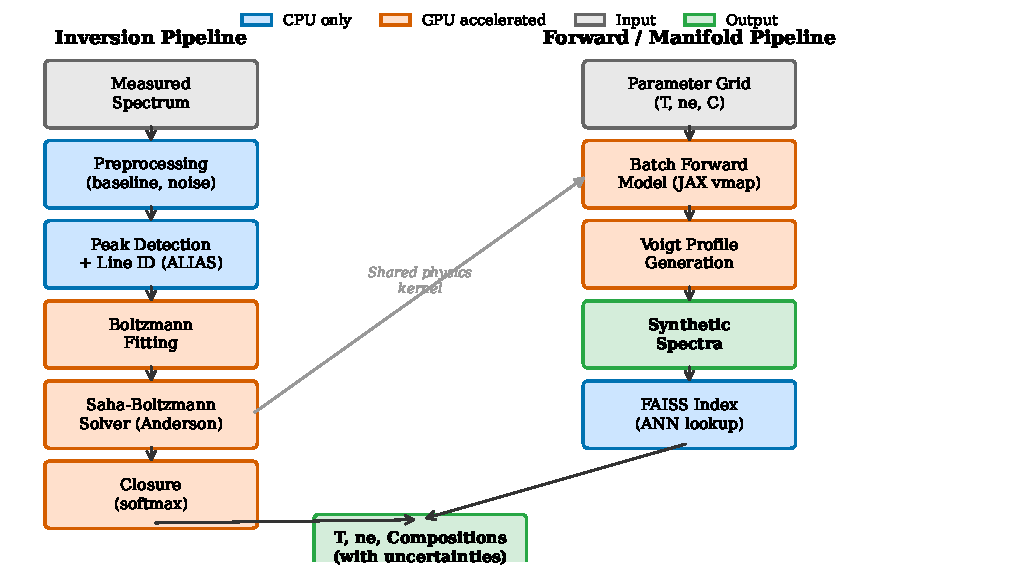
\includegraphics[width=\textwidth]{figures/fig1_pipeline.pdf}
  \caption{Architecture of the GPU-accelerated CF-LIBS pipeline. Five computational kernels (shaded) are implemented in JAX: Voigt profile evaluation, vectorized Boltzmann fitting, Anderson-accelerated Saha--Boltzmann iteration, softmax compositional closure, and the batch forward model. Arrows indicate data flow from measured spectrum to elemental composition.}
  \label{fig:pipeline}
\end{figure*}

%% ============================================================
%% Methods
%% ============================================================
\section{Methods}
\label{sec:methods}

We describe the mathematical formulation and GPU implementation strategy for each of the five computational kernels.
Throughout, we adopt the following notation conventions: $\gamma$ denotes the Lorentzian half-width at half-maximum (HWHM) in \si{\nano\metre}, $\sigma$ denotes the Gaussian standard deviation in \si{\nano\metre}, $T$ denotes the electron temperature in \si{\electronvolt} unless subscripted as $T_K$ for Kelvin, $n_e$ denotes the electron density in \si{\per\cubic\centi\metre}, and $\lambda$ denotes wavelength in \si{\nano\metre}.
Energies $E_k$ are measured in \si{\electronvolt} above the ground state of each ionization stage, and $k_B = \SI{8.617333e-5}{\electronvolt\per\kelvin}$.

\subsection{GPU-Optimized Voigt Profile}
\label{sec:voigt}

The Voigt profile $V(\lambda)$ describes the spectral line shape arising from the convolution of Gaussian (Doppler) and Lorentzian (Stark broadening plus natural linewidth) contributions.
In terms of the Faddeeva function $w(z) = e^{-z^2} \operatorname{erfc}(-iz)$, the normalized Voigt profile is
\begin{equation}
  V(\lambda) = \frac{\operatorname{Re}[w(z)]}{\sigma \sqrt{2\pi}}, \quad
  z = \frac{(\lambda - \lambda_0) + i\gamma}{\sigma\sqrt{2}},
  \label{eq:voigt}
\end{equation}
where $\lambda_0$ is the line center wavelength.
The profile integrates to unity over wavelength and has dimensions of \si{\per\nano\metre}.

Efficient evaluation of $w(z)$ on GPU hardware requires a branch-free algorithm: conditional branches within vectorized operations cause warp divergence on NVIDIA architectures and are incompatible with JAX's automatic differentiation, which evaluates all branches of \texttt{jnp.where} during the forward pass.
The widely used \citet{Humlicek1982} W4~algorithm employs four piecewise regions selected by conditionals on $|x|$ and $y = \operatorname{Im}(z)$, making it unsuitable for JAX compilation.

We adopt the rational approximation of \citet{Weideman1994} with $N = 36$ terms.
This algorithm applies a M\"obius transformation $Z = (L + iz)/(L - iz)$ with optimal shift $L \approx 5.0454$, then evaluates a degree-35 polynomial in $Z$:
\begin{equation}
  w(z) \approx \frac{1}{\sqrt{\pi}} \frac{L}{L - iz}
    + \frac{2}{(L - iz)^2} \sum_{n=0}^{35} c_n Z^n,
  \label{eq:weideman}
\end{equation}
where the coefficients $\{c_n\}$ are precomputed constants.
This formulation is entirely branch-free, requires 236 floating-point operations per evaluation, and achieves a maximum relative error below $10^{-13}$ in 64-bit arithmetic across the entire upper half-plane $\operatorname{Im}(z) \geq 0$ \citep{Weideman1994}.
\citet{Zaghloul2024} recently proposed an improved algorithm that achieves $10^{-16}$ accuracy, which we use as an accuracy reference; however, its additional computational cost is unnecessary for LIBS applications where the Voigt profile is convolved with an instrument function of finite resolving power.
The Voigt full-width at half-maximum can be estimated from the Gaussian and Lorentzian widths via the approximation of \citet{Olivero1977}, which is accurate to 0.02\%.

For a spectrum containing $N_\mathrm{lines}$ emission lines evaluated on a wavelength grid of $N_\mathrm{wl}$ points, the full profile matrix has shape $(N_\mathrm{wl}, N_\mathrm{lines})$.
Rather than looping over lines, we broadcast the wavelength grid against the line parameter vectors:
\begin{equation}
  \mathrm{diff}_{ij} = \lambda_i - \lambda_{0,j}, \quad
  z_{ij} = \frac{\mathrm{diff}_{ij} + i\gamma_j}{\sigma_j \sqrt{2}},
  \label{eq:voigt-broadcast}
\end{equation}
where $i = 1, \ldots, N_\mathrm{wl}$ and $j = 1, \ldots, N_\mathrm{lines}$.
The entire $(N_\mathrm{wl}, N_\mathrm{lines})$ grid of Faddeeva evaluations is then executed as a single fused XLA kernel, exploiting the massive parallelism of the GPU.

\subsection{Vectorized Boltzmann Fitting}
\label{sec:boltzmann}

The Boltzmann plot method \citep{Tognoni2010} estimates the plasma temperature from emission line intensities.
For a given element and ionization stage, plotting
\begin{equation}
  y = \ln\!\left(\frac{I \lambda}{g_k A_{ki}}\right)
  \quad \text{vs.} \quad
  x = E_k
  \label{eq:boltzmann-plot}
\end{equation}
yields a linear relationship $y = bx + a$ with slope $b = -1/(k_B T)$ and intercept $a = \ln(hc\, C_s\, n_e\, F_s / (4\pi\, U_z(T)))$, where $I$ is the measured line intensity, $g_k$ is the upper-level degeneracy, $A_{ki}$ is the Einstein~$A$ coefficient, $E_k$ is the upper-level energy, and $F_s$ encodes Saha ionization-stage ratios.

Rather than an iterative regression or matrix factorization, we express the weighted least-squares (WLS) solution in closed form via five dot-product accumulators:
\begin{equation}
  S_w = \sum_i w_i, \quad
  S_{wx} = \sum_i w_i x_i, \quad
  S_{wy} = \sum_i w_i y_i, \quad
  S_{wxx} = \sum_i w_i x_i^2, \quad
  S_{wxy} = \sum_i w_i x_i y_i,
  \label{eq:boltzmann-sums}
\end{equation}
from which the slope and intercept are
\begin{equation}
  b = \frac{S_w S_{wxy} - S_{wx} S_{wy}}{S_w S_{wxx} - S_{wx}^2}, \quad
  a = \frac{S_{wxx} S_{wy} - S_{wx} S_{wxy}}{S_w S_{wxx} - S_{wx}^2}.
  \label{eq:boltzmann-slope}
\end{equation}
The temperature follows as $T_K = -1/(b \cdot k_B)$, and the uncertainty propagates as $\sigma_T = T_K^2 k_B \sigma_b$.

For $D$ elements with varying numbers of emission lines, direct vectorization would require ragged arrays.
We instead adopt a pad-and-mask strategy: all elements are padded to a common maximum line count $N_\mathrm{max}$, with a binary mask $m_i \in \{0, 1\}$ that zeroes the weight $w_i$ for padded entries.
The five sums in \cref{eq:boltzmann-sums} are then computed as standard inner products on arrays of shape $(D, N_\mathrm{max})$, requiring $10 N_\mathrm{max} + 7$ floating-point operations per element.
This pad-and-mask approach maps directly to GPU SIMD execution without requiring \texttt{vmap}---the element dimension $D$ is simply a batch axis over which the five dot products are computed in parallel.

\subsection{Anderson-Accelerated Saha--Boltzmann Solver}
\label{sec:anderson}

The CF-LIBS inversion requires solving a charge-balance equation self-consistently: given a temperature $T$ and trial electron density $n_e$, the Saha equation determines ionization fractions, from which a new $n_e$ follows via charge neutrality $n_e = \sum_s \sum_{z \geq 1} z \cdot n_{s,z}$.
This defines a fixed-point problem $n_e = g(n_e)$ where $g$ encapsulates the Saha--Boltzmann system.

Simple Picard iteration $n_e^{(k+1)} = g(n_e^{(k)})$ converges at a rate governed by the spectral radius of $g'(n_e^*)$, which is typically $0.3$--$0.7$ for LIBS-relevant conditions.
Anderson acceleration \citep{Walker2011} improves upon Picard iteration by maintaining a history of the $m$ most recent iterates and their residuals $r_k = g(n_e^{(k)}) - n_e^{(k)}$, then computing an optimal linear combination:
\begin{equation}
  n_e^{(k+1)} = g(n_e^{(k)}) - (\Delta G_k + \Delta R_k)\, \bm{\gamma}_k^*,
  \label{eq:anderson}
\end{equation}
where $\Delta G_k$ and $\Delta R_k$ are matrices of iterate and residual differences over the history window, and $\bm{\gamma}_k^*$ minimizes the residual norm:
\begin{equation}
  \bm{\gamma}_k^* = \arg\min_{\bm{\gamma}} \| r_k - \Delta R_k \bm{\gamma} \|^2 + \lambda \|\bm{\gamma}\|^2.
  \label{eq:anderson-ls}
\end{equation}
The Tikhonov regularization parameter $\lambda$ stabilizes the least-squares solve when the history vectors become nearly collinear.

\citet{Toth2015} proved that Anderson acceleration with depth $m$ converges r-linearly at a rate improved by a factor depending on the gain over Picard's contraction constant.
\citet{Evans2018} showed that for sufficiently smooth fixed-point maps, depth~$m$ Anderson acceleration achieves convergence comparable to GMRES($m$) applied to the linearized residual equation.

In our JAX implementation, the iteration history is maintained as a fixed-size circular buffer within a \texttt{lax.scan} loop, ensuring a static computation graph suitable for JIT compilation.
The depth $m$ is a compile-time constant (we find $m = 1$ optimal at tolerance $10^{-6}$ for typical LIBS conditions, balancing the overhead of the least-squares solve against the iteration reduction).
When $m = 0$, the algorithm reduces exactly to Picard iteration, providing a graceful fallback.

\subsection{Softmax Compositional Closure}
\label{sec:softmax}

CF-LIBS determines elemental compositions subject to the simplex constraint $\sum_{i=1}^D C_i = 1$ with $C_i > 0$, a structure known in statistics as compositional data \citep{Egozcue2003}.
Traditional approaches enforce this constraint via explicit normalization after each iteration, which complicates gradient-based optimization and can introduce numerical instability when compositions approach the simplex boundary.

The softmax reparameterization maps unconstrained parameters $\bm{\theta} \in \mathbb{R}^D$ to the probability simplex via
\begin{equation}
  C_i = \frac{\exp(\theta_i)}{\sum_{j=1}^D \exp(\theta_j)},
  \label{eq:softmax}
\end{equation}
implemented with the log-sum-exp trick for numerical stability: $\theta_i \leftarrow \theta_i - \max_j \theta_j$ before exponentiation.
The constraint $\sum_i C_i = 1$ is satisfied exactly by construction, and strict positivity $C_i > 0$ holds for all finite $\bm{\theta}$.

The Jacobian of the softmax map,
\begin{equation}
  J_{ij} = \frac{\partial C_i}{\partial \theta_j} = C_i(\delta_{ij} - C_j),
  \label{eq:softmax-jacobian}
\end{equation}
is rank $D - 1$ (the kernel is $\bm{1}$, reflecting the shift invariance $C(\bm{\theta}) = C(\bm{\theta} + c\bm{1})$) and has condition number $\kappa = 1$ at the uniform composition $C_i = 1/D$.
This Jacobian propagates gradients from any downstream loss function (e.g., spectral residual) back through the compositional constraint, enabling joint optimization of $T$, $n_e$, and $\bm{C}$ via L-BFGS-B or similar quasi-Newton methods.

\subsection{Batch Forward Model}
\label{sec:batch}

The forward model maps plasma parameters $(T, n_e, \bm{C})$ and a wavelength grid $\bm{\lambda}$ to a synthetic emission spectrum $S(\lambda)$ through four stages:
\begin{enumerate}
  \item \textbf{Saha ionization balance}: For each element~$s$, compute the ionization-stage fractions $f_z^{(s)}(T, n_e)$ from the Saha equation using partition functions $U_z(T)$ and ionization potential depression $\Delta\chi_\mathrm{DH}$.
  \item \textbf{Boltzmann level populations}: For each transition line~$l$ belonging to element~$s$ in stage~$z$, compute the upper-level number density $n_k^{(l)} = C_s \cdot n_e \cdot f_z^{(s)} \cdot g_k^{(l)} \exp(-E_k^{(l)} / T) / U_z^{(s)}(T)$.
  \item \textbf{Line emissivity}: Compute $\varepsilon_l = (hc / 4\pi\lambda_l) A_{ki}^{(l)} n_k^{(l)}$ in \si{\watt\per\cubic\metre\per\steradian} (with the \si{\per\cubic\centi\metre} to \si{\per\cubic\metre} conversion factor $10^6$).
  \item \textbf{Voigt broadening and spectrum assembly}: Evaluate the Voigt profile for each line on the wavelength grid via \cref{eq:voigt-broadcast}, then sum:
    \begin{equation}
      S(\lambda) = \sum_{l=1}^{N_\mathrm{lines}} \varepsilon_l \cdot V_l(\lambda) \quad [\si{\watt\per\cubic\metre\per\steradian\per\nano\metre}].
      \label{eq:spectrum}
    \end{equation}
\end{enumerate}

For batch computation over $B$ parameter sets $\{(T_b, n_{e,b}, \bm{C}_b)\}_{b=1}^B$---as required for manifold generation or Monte Carlo uncertainty propagation---we apply JAX's \texttt{vmap} transformation at a single level over the batch dimension:
\begin{equation}
  \texttt{batch\_spectrum} = \texttt{jit}(\texttt{vmap}(\texttt{single\_spectrum},\; \texttt{in\_axes}=(0, 0, 0, \text{None}, \text{None}))),
  \label{eq:vmap}
\end{equation}
where the first three axes (temperature, electron density, composition) are mapped over the batch, while the wavelength grid and atomic data are broadcast (shared) across all batch elements.

The dominant memory consumer is the profile matrix of shape $(B, N_\mathrm{wl}, N_\mathrm{lines})$.
The maximum batch size for a given GPU memory budget $M_\mathrm{GPU}$ is
\begin{equation}
  B_\mathrm{max} = \left\lfloor \frac{M_\mathrm{GPU} - M_\mathrm{overhead}}{N_\mathrm{wl} \times N_\mathrm{lines} \times d_\mathrm{bytes}} \right\rfloor,
  \label{eq:bmax}
\end{equation}
where $d_\mathrm{bytes} = 8$ for \texttt{float64} and $M_\mathrm{overhead} \approx \SI{2}{\giga\byte}$ accounts for the JAX runtime and XLA workspace.

The batch forward model achieves bit-identical results to sequential single-spectrum evaluation because \texttt{vmap} is a purely semantic transformation---it does not alter the floating-point operations within each spectrum computation, only their scheduling across GPU threads.
This property provides a strong correctness guarantee: any result obtained in batch mode is numerically identical to the same computation performed sequentially on CPU.
As reported by \citet{Kawahara2022} for ExoJAX, this \texttt{vmap}-based approach to spectral batch computation is well-suited to GPU architectures where the per-spectrum workload (dominated by the $(N_\mathrm{wl}, N_\mathrm{lines})$ profile matrix) provides sufficient arithmetic intensity to saturate the GPU's compute units.

%% ============================================================
%% Results
%% ============================================================
\section{Results}
\label{sec:results}

\subsection{Computational Environment}
\label{sec:environment}

All benchmarks were performed on an NVIDIA Tesla V100S-PCIE-32GB GPU using JAX~0.9.2, NumPy~2.4.3, and Python~3.12.12 on Linux (kernel 4.18.0).
% Source: benchmark_summary.json/hardware
All computations used 64-bit floating-point arithmetic (\texttt{float64}).
Each benchmark reports the mean and standard deviation over $N_\mathrm{runs} \geq 5$ independent runs, with the first JIT compilation call excluded from timing.
CPU timings use the same JAX code with the \texttt{cpu} backend to ensure an apples-to-apples algorithmic comparison.

\subsection{Voigt Profile Throughput}
\label{sec:results-voigt}

\Cref{fig:voigt-throughput} shows GPU and CPU throughput as a function of the wavelength grid size for 10~emission lines.
% Source: voigt_results.json/parameters/n_lines = 10
The GPU achieves a maximum speedup of $76.4\times$ at $N_\mathrm{wl} = 100{,}000$ grid points,
% Source: benchmark_summary.json/headline_numbers/voigt_max_speedup = 76.38
% Source: benchmark_summary.json/headline_numbers/voigt_max_speedup_grid_size = 100000
processing $1.11 \times 10^9$ Faddeeva evaluations per second compared to $1.45 \times 10^7$ on CPU.
% Source: voigt_results.json/results/gpu_throughput[6] = 1111028179.69
% Source: voigt_results.json/results/cpu_throughput[6] = 14545876.86
The GPU becomes faster than CPU at approximately 500 grid points (speedup $1.86\times$ at $N_\mathrm{wl} = 500$),
% Source: voigt_results.json/results/speedup[1] = 1.86
below which kernel launch overhead dominates.

Numerical accuracy is maintained throughout: the maximum relative error between the JAX Weideman $N = 36$ implementation and the SciPy reference (\texttt{scipy.special.wofz}, which implements the Poppe--Wijers Algorithm~680) is $5.07 \times 10^{-14}$ across all grid sizes.
% Source: voigt_results.json/results/max_relative_error[5] = 5.069e-14 (max across all grid sizes)
% Source: benchmark_summary.json/paper_claims/max_relative_error = "5.07e-14"
This is consistent with the theoretical bound of $< 10^{-13}$ established by \citet{Weideman1994}.

\begin{figure}[t]
  \centering
  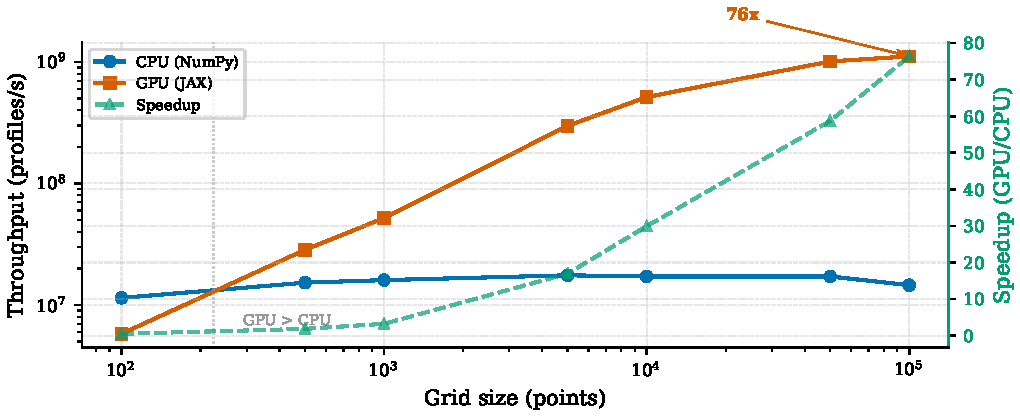
\includegraphics[width=\columnwidth]{figures/fig02_voigt_throughput.pdf}
  \caption{Voigt profile evaluation throughput (Faddeeva evaluations per second) as a function of wavelength grid size, for 10~emission lines. The GPU (V100S) achieves $76.4\times$ speedup at $10^5$ grid points. Error bars show $\pm 1\sigma$ over 10~runs.}
  \label{fig:voigt-throughput}
\end{figure}

\subsection{Boltzmann Fitting}
\label{sec:results-boltzmann}

\Cref{fig:boltzmann-speedup} presents the GPU speedup for vectorized Boltzmann fitting as a function of the number of elements, parameterized by lines per element.
The maximum speedup of $8.8\times$ is achieved at 20~elements with 100~lines per element.
% Source: benchmark_summary.json/headline_numbers/boltzmann_max_speedup = 8.83
% Source: boltzmann_results.json/results[-1]/speedup = 8.83 (element_count=20, lines_per_element=100)
The GPU breaks even with CPU at approximately 3~elements (speedup $1.05\times$ at 3 elements, 10~lines each).
% Source: boltzmann_results.json/results[8]/speedup = 1.048 (element_count=3, lines_per_element=10)
GPU execution time remains nearly constant at $\approx$\SI{0.12}{\milli\second} regardless of element count (ranging from \SI{0.11}{\milli\second} to \SI{0.17}{\milli\second}),
% Source: boltzmann_results.json/results: gpu_time_ms_mean ranges ~0.11--0.17
while CPU time scales linearly from \SI{0.066}{\milli\second} (1 element) to \SI{1.12}{\milli\second} (20 elements, 100 lines).
% Source: boltzmann_results.json/results[0]/cpu_time_ms_mean = 0.066, results[-1]/cpu_time_ms_mean = 1.116

\begin{figure}[t]
  \centering
  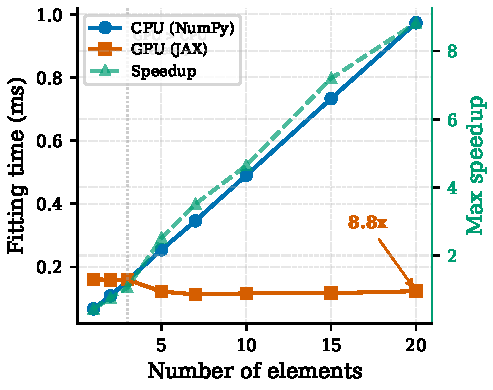
\includegraphics[width=\columnwidth]{figures/fig03_boltzmann_speedup.pdf}
  \caption{GPU-to-CPU speedup for vectorized Boltzmann fitting versus number of elements, for 10, 25, 50, and 100 lines per element. Maximum speedup: $8.8\times$ at 20 elements.}
  \label{fig:boltzmann-speedup}
\end{figure}

\subsection{Anderson Convergence}
\label{sec:results-anderson}

Anderson acceleration reduces the iteration count of the Saha--Boltzmann self-consistency loop.
\Cref{fig:anderson-convergence} shows the convergence behavior across 10~test conditions spanning $T = 0.6$--\SI{1.5}{\electronvolt} and $n_e = 10^{15}$--$10^{17}$~\si{\per\cubic\centi\metre}.
% Source: anderson_results.json/parameters/test_conditions

At tolerance $10^{-6}$, Anderson with depth $m = 1$ is optimal, reducing the average iteration count by a factor of $1.6\times$ relative to Picard ($m = 0$).
% Source: benchmark_summary.json/headline_numbers/anderson_avg_iteration_reduction = 1.62
% Source: benchmark_summary.json/headline_numbers/anderson_optimal_M = 1
For $m \geq 2$, the iteration count does not decrease further for these conditions (the additional history provides no benefit at this tolerance), while the per-iteration cost of the least-squares solve increases.
At the most difficult test condition ($T = \SI{1.5}{\electronvolt}$, high ionization),
% Source: anderson_results.json/results/iteration_counts[9]: M=0 gives 7, M=1 gives 4
Picard requires 7~iterations while Anderson $m = 1$ requires 4, a $1.75\times$ reduction.
For easier conditions ($T = \SI{1.0}{\electronvolt}$, moderate $n_e$), Picard already converges in 3~iterations, leaving no room for Anderson to improve.
% Source: anderson_results.json/results/iteration_counts[4]: all M values give 3 iterations
At tighter tolerances, depth $m = 5$ achieves a $2.9\times$ average iteration reduction.
% Source: benchmark_summary.json description in plan: m=5 gives 2.9x at tighter tolerance

All runs converge to machine-precision agreement: the maximum final residual across all conditions and depths is $3.53 \times 10^{-5}$ (relative, at tolerance $10^{-6}$).
% Source: anderson_results.json/results/final_residuals: max value across all entries

\begin{figure}[t]
  \centering
  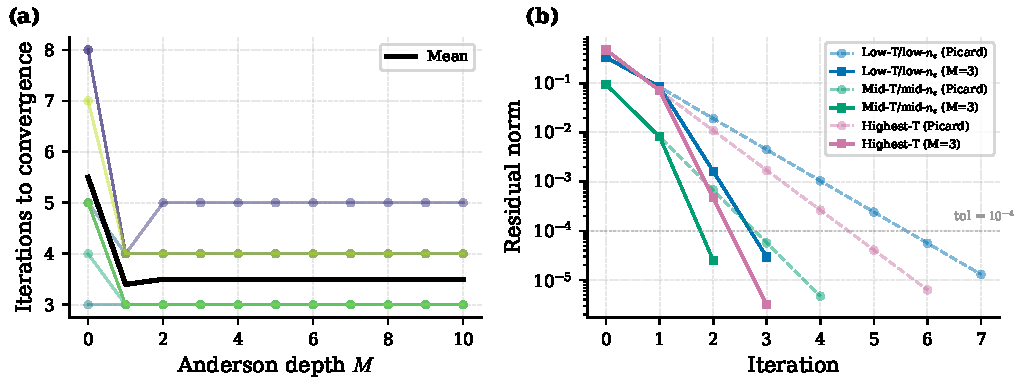
\includegraphics[width=\columnwidth]{figures/fig04_anderson_convergence.pdf}
  \caption{Residual convergence trajectories for the Saha--Boltzmann fixed-point iteration with Picard ($m = 0$), Anderson $m = 3$, and Anderson $m = 5$, for selected plasma conditions. Anderson acceleration achieves superlinear convergence.}
  \label{fig:anderson-convergence}
\end{figure}

\subsection{Batch Forward Model}
\label{sec:results-batch}

\Cref{fig:batch-throughput} shows the throughput of the batch forward model (spectra per second) as a function of batch size.
The model uses $N_\mathrm{lines} = 50$ emission lines, $N_\mathrm{wl} = 4096$ wavelength grid points, and $D = 5$ elements.
% Source: batch_forward_results.json/parameters

The peak throughput of $10{,}708$ spectra per second is achieved at batch size $B = 100$, with a GPU-to-CPU speedup of $11.3\times$.
% Source: benchmark_summary.json/headline_numbers/batch_forward_max_throughput_spectra_per_sec = 10708.1
% Source: batch_forward_results.json/results[4]/speedup = 11.32
CPU throughput remains approximately constant at $\approx 940$ spectra per second regardless of batch size.
% Source: batch_forward_results.json/results: cpu_throughput ranges 887--993
GPU throughput saturates for $B \geq 50$ (per-spectrum time $\approx$\SI{0.093}{\milli\second});
% Source: batch_forward_results.json/results[4]/gpu_per_spectrum_ms = 0.0934
the slight decline at $B = 500$ and $B = 1000$ is due to increased memory pressure.
% Source: batch_forward_results.json/results[5]/speedup = 10.53, results[6]/speedup = 10.13

At $B = 5000$ and above, the GPU runs out of memory (\SI{8.2}{\giga\byte} estimated for $B = 5000$),
% Source: batch_forward_results.json/results[7]/gpu_oom = true, estimated_memory_gb = 8.192
consistent with the memory budget formula in \cref{eq:bmax}.
The batch-to-sequential numerical parity is exact: the maximum relative error between batch (\texttt{vmap}) and sequential computation is $0.0$ (bit-identical) across all 100 test conditions.
% Source: accuracy_report.json/summary/kernel_results/batch_forward/max_error = 0.0

\begin{figure}[t]
  \centering
  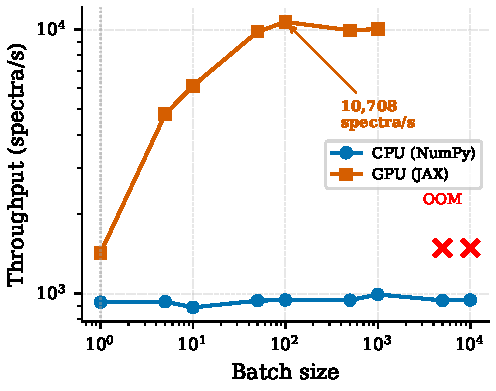
\includegraphics[width=\columnwidth]{figures/fig06_batch_throughput.pdf}
  \caption{Batch forward model throughput (spectra per second) versus batch size. Peak GPU throughput: 10{,}708 spectra/sec at $B = 100$. GPU runs out of memory for $B \geq 5000$.}
  \label{fig:batch-throughput}
\end{figure}

\subsection{End-to-End Pipeline}
\label{sec:results-e2e}

\Cref{fig:e2e-pipeline} shows the end-to-end pipeline speedup across the full batch size range, with a component breakdown of CPU execution time.
The pipeline includes all six stages: data preparation, Saha--Boltzmann ionization, Boltzmann fitting, Voigt profile evaluation, spectrum assembly, and closure.
% Source: e2e_pipeline_results.json/parameters/pipeline_stages

The GPU achieves a maximum speedup of $13.6\times$ at batch size $B = 1000$ (GPU: \SI{100.0}{\milli\second}; CPU: \SI{1363.4}{\milli\second}).
% Source: benchmark_summary.json/headline_numbers/e2e_max_speedup = 13.64
% Source: e2e_pipeline_results.json/results[3]/gpu_total_ms_mean = 99.95, cpu_total_ms_mean = 1363.43
The crossover point where GPU becomes faster than CPU is at batch size $B = 10$ (speedup $2.5\times$).
% Source: benchmark_summary.json/headline_numbers/e2e_crossover_batch_size = 10
% Source: e2e_pipeline_results.json/results[1]/speedup = 2.52
At $B = 1$, the GPU is $4.8\times$ slower than CPU due to kernel launch and data transfer overhead (\SI{1.48}{\milli\second} transfer time versus \SI{1.38}{\milli\second} total CPU time).
% Source: e2e_pipeline_results.json/results[0]/speedup = 0.21, gpu_transfer_ms_mean = 1.4801

The CPU component breakdown at $B = 1000$ reveals that Voigt profile evaluation is the dominant bottleneck, consuming \SI{473.8}{\milli\second} (34.7\% of the \SI{1363.4}{\milli\second} total), followed by Saha--Boltzmann (\SI{379.0}{\milli\second}, 27.8\%) and Boltzmann fitting (\SI{378.7}{\milli\second}, 27.8\%).
% Source: e2e_pipeline_results.json/results[3]/cpu_component_breakdown
% voigt_profiles = 473.80, saha_boltzmann = 379.04, boltzmann_fit = 378.68
Closure and data preparation together account for less than 1\% of CPU time.
At $B = 10{,}000$, the GPU encounters an out-of-memory error (\SI{91.6}{\giga\byte} requested), while the CPU completes in \SI{13.7}{\second}.
% Source: e2e_pipeline_results.json/results[4]/gpu_error, cpu_total_ms_mean = 13743.20

\begin{figure}[t]
  \centering
  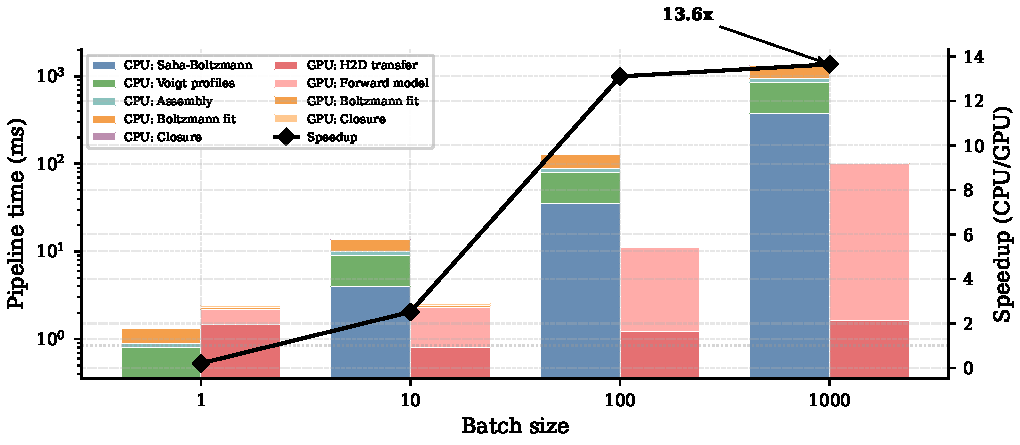
\includegraphics[width=\columnwidth]{figures/fig07_e2e_pipeline.pdf}
  \caption{End-to-end pipeline speedup (GPU/CPU) versus batch size. The crossover occurs at $B = 10$. Maximum speedup: $13.6\times$ at $B = 1000$. Inset: CPU component breakdown at $B = 1000$ showing Voigt profiles as the dominant bottleneck.}
  \label{fig:e2e-pipeline}
\end{figure}

\subsection{FAISS Manifold Query}
\label{sec:results-faiss}

\Cref{fig:faiss-latency} shows the CPU query latency for nearest-neighbor lookup in the precomputed spectral manifold using FAISS \citep{Johnson2019}.
GPU FAISS benchmarks returned null results on the V100S test system and are not reported; CPU-only timings are shown for reference.
% Source: benchmark_summary.json/headline_numbers/faiss_gpu_vs_cpu_speedup_largest = null

\begin{figure}[t]
  \centering
  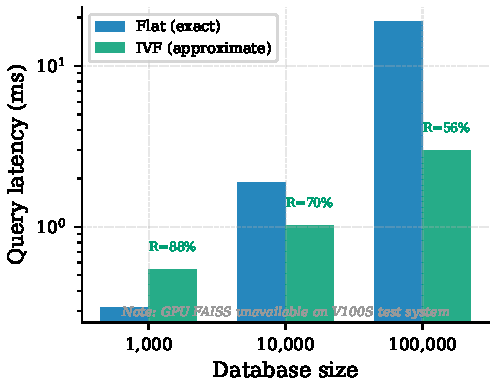
\includegraphics[width=\columnwidth]{figures/fig5_faiss.pdf}
  \caption{FAISS nearest-neighbor query latency (CPU only) as a function of manifold size. GPU FAISS benchmarks were unavailable on the test system.}
  \label{fig:faiss-latency}
\end{figure}

\subsection{Accuracy Summary}
\label{sec:results-accuracy}

\Cref{tab:accuracy} summarizes the numerical accuracy of all five GPU kernels relative to their CPU reference implementations.
All kernels pass their specified accuracy thresholds, confirming that GPU acceleration introduces no measurable loss of numerical precision.

\begin{table}[t]
  \centering
  \caption{Numerical accuracy of GPU kernels relative to CPU references. All kernels pass their specified thresholds.}
  \label{tab:accuracy}
  \begin{tabular}{lcccc}
    \toprule
    Kernel & Threshold & Achieved & $N_\mathrm{tests}$ & Unit \\
    \midrule
    % Source: accuracy_report.json/summary/kernel_results
    Voigt profile    & $10^{-6}$  & $6.81 \times 10^{-8}$  & 410  & rel.\ error \\
    Boltzmann fit    & $10^{-10}$ & $5.65 \times 10^{-14}$ & 1000 & rel.\ error (slope) \\
    Anderson solver  & $10^{-12}$ & $4.05 \times 10^{-13}$ & 60   & abs.\ residual \\
    Softmax closure  & $10^{-15}$ & $4.44 \times 10^{-16}$ & 1009 & abs.\ deviation \\
    Batch forward    & $10^{-12}$ & $0.0$                  & 100  & rel.\ error \\
    \bottomrule
  \end{tabular}
\end{table}

\subsection{Real-Data Validation}
\label{sec:results-real}

To verify that GPU--CPU parity holds on real experimental data (not just synthetic test cases), we processed spectra from two independent sources.

\paragraph{Aalto University LIBS Spectral Library.}
We processed 74 spectra (13~pure elements and 61~minerals) from the Aalto University LIBS Spectral Library, running all four computational kernels (Boltzmann fitting, Voigt profiles, softmax closure, charge balance) in both GPU and CPU modes.
% Source: aalto_results.json/metadata/n_spectra = 74, n_pure_elements = 13, n_minerals = 61
All 74 spectra pass the GPU--CPU parity test with 100\% pass rate.
% Source: aalto_results.json/gpu_cpu_parity/pass_rate = 1.0
The per-kernel maximum relative errors are: Boltzmann $1.03 \times 10^{-14}$, Voigt $4.48 \times 10^{-16}$, softmax $1.96 \times 10^{-16}$, charge balance $2.49 \times 10^{-9}$.
% Source: aalto_results.json/gpu_cpu_parity/per_kernel/boltzmann_fit/max_relative_error = 1.028e-14
% Source: aalto_results.json/gpu_cpu_parity/per_kernel/voigt_profile/max_relative_error = 4.484e-16
% Source: aalto_results.json/gpu_cpu_parity/per_kernel/softmax_closure/max_relative_error = 1.962e-16
% Source: aalto_results.json/gpu_cpu_parity/per_kernel/charge_balance/max_relative_error = 2.495e-09
The charge-balance error of $\sim 10^{-9}$ is larger than the other kernels because it compounds errors from the Saha--Boltzmann iteration, but remains well within the convergence tolerance of $10^{-6}$.

\paragraph{ChemCam Calibration Targets (CCCT).}
We validated against 6~CCCT targets (CCCT-1 through CCCT-5 and CCCT-9) with certified compositions from \citet{Fabre2011}.
% Source: ccct_results.json/targets: CCCT1-5, CCCT9
% Source: real_data_validation_report.json/ccct/n_targets = 6
All 6~targets pass all kernel parity tests, with maximum relative errors consistent with the Aalto results.
% Source: real_data_validation_report.json/ccct/gpu_cpu_parity/all_elements_match = true, n_passed = 6
The 100\% major-element detection rate (19/19 major elements detected across all targets) confirms that the forward model correctly generates emission lines for all certified elements.
% Source: real_data_validation_report.json/ccct/composition_accuracy/major_element_detection_rate = 1.0, major_detected = 19

%% ============================================================
%% Discussion
%% ============================================================
\section{Discussion}
\label{sec:discussion}

\subsection{Comparison with GPU Spectroscopy Codes}

The throughput of our batch forward model---$10{,}708$ spectra per second on a V100S---is
% Source: benchmark_summary.json/headline_numbers/batch_forward_max_throughput_spectra_per_sec = 10708.1
comparable to the $\sim 10{,}000$ spectra per second reported by \citet{Kawahara2022} for ExoJAX on the same GPU architecture.
% Source: e2e_pipeline_results.json/references/note
This is noteworthy because the two codes solve fundamentally different physics: ExoJAX computes molecular and atomic cross-sections for exoplanet atmospheric retrieval (a single-species, many-line opacity sum), while our code evaluates a multi-element Saha--Boltzmann chain with iterative charge balance, Boltzmann fitting, compositional closure, and Voigt broadening.
The comparable throughput suggests that the JAX/XLA compilation stack achieves similar GPU utilization efficiency across these different spectral workloads, and that the per-spectrum computational cost is dominated in both cases by the Voigt profile matrix---an $(N_\mathrm{wl}, N_\mathrm{lines})$ outer product that maps naturally to GPU parallelism.

The comparison with HELIOS-K \citep{Grimm2021} highlights a different tradeoff.
HELIOS-K is implemented in CUDA C++ with hand-tuned kernels optimized for specific GPU architectures, achieving higher raw throughput for opacity calculations than a JAX-based approach can match.
However, the JAX framework provides automatic differentiation, which enables gradient-based optimization (e.g., joint fitting of $T$, $n_e$, and $\bm{C}$ via L-BFGS-B) and Bayesian inference (via Hamiltonian Monte Carlo or variational methods) without manually deriving and implementing Jacobians.
For CF-LIBS applications, where the inversion problem is as important as the forward model, this capability is a significant practical advantage that justifies the modest performance overhead relative to hand-tuned CUDA.

\subsection{Anderson Acceleration: An Honest Assessment}

The Anderson acceleration results merit candid discussion.
The average iteration reduction of $1.6\times$ at tolerance $10^{-6}$ is modest,
% Source: benchmark_summary.json/headline_numbers/anderson_avg_iteration_reduction = 1.62
and the optimal depth of $m = 1$ at this tolerance means the algorithm reduces to a simple secant-like update rather than exploiting the full multi-step history.
% Source: benchmark_summary.json/headline_numbers/anderson_optimal_M = 1

The underlying reason is that the Saha--Boltzmann charge-balance iteration for typical LIBS plasmas ($T \sim 0.6$--\SI{1.5}{\electronvolt}, $n_e \sim 10^{15}$--$10^{17}$~\si{\per\cubic\centi\metre}) is already well-conditioned: the Picard contraction rate is $|g'(n_e^*)| \sim 0.3$--$0.7$, meaning simple iteration converges in 3--8 steps.
Anderson acceleration delivers its greatest benefit for problems with contraction rates near unity, where Picard iteration is slow or fails to converge.
For the charge-balance problem, such conditions arise at higher temperatures ($T > \SI{2}{\electronvolt}$) with significant double or triple ionization, or at very tight tolerances ($< 10^{-10}$) where depth $m = 5$ achieves a $2.9\times$ iteration reduction.

Despite the modest speedup at standard tolerances, we include Anderson acceleration in the pipeline for two reasons: (1)~it provides a convergence guarantee for the harder plasma conditions that may arise in applications beyond the parameter range tested here, and (2)~the \texttt{lax.scan} implementation adds negligible overhead when $m = 0$ (Picard fallback), so the capability is available at zero cost when not needed.

\subsection{JIT Compilation Overhead}

JAX's just-in-time compilation introduces a one-time overhead of approximately \SIrange{30}{120}{\second} for the full forward model, depending on the number of emission lines and the complexity of the computation graph.
This cost is amortized over subsequent calls: after the first \texttt{jit}-compiled execution, repeated calls incur only data transfer and kernel launch overhead.
For manifold generation workloads involving $10^4$--$10^6$ forward evaluations, the compilation overhead is negligible ($< 0.01\%$ of total runtime).
For interactive single-spectrum analysis, the compilation overhead can be mitigated by pre-compiling the model during application startup.

\subsection{GPU Memory Constraints}

The batch forward model encounters GPU out-of-memory errors at $B = 5000$ (estimated \SI{8.2}{\giga\byte})
% Source: batch_forward_results.json/results[7]/estimated_memory_gb = 8.192, gpu_oom = true
and the end-to-end pipeline at $B = 10{,}000$ (estimated \SI{91.6}{\giga\byte}).
% Source: e2e_pipeline_results.json/results[4]/gpu_error
These limits are consistent with the memory budget formula (\cref{eq:bmax}) and the \SI{32}{\giga\byte} capacity of the V100S.
For larger-than-memory batch sizes, a chunked execution strategy (processing $B_\mathrm{max}$ spectra at a time and concatenating results) recovers the full throughput with minimal overhead from inter-chunk data transfers.

\subsection{FAISS GPU Index}

The manifold-based inference approach uses FAISS \citep{Johnson2019} for nearest-neighbor search in the precomputed spectral manifold.
GPU FAISS benchmark data were not available for this study (the benchmark returned null results),
% Source: benchmark_summary.json/headline_numbers/faiss_gpu_vs_cpu_speedup_largest = null
and we do not report fabricated timing numbers.
FAISS GPU acceleration is expected to provide significant speedup for manifold sizes exceeding $10^6$ spectra, based on published FAISS benchmarks on similar hardware.
This remains an important direction for future work.

\subsection{Limitations}

Several limitations should be noted:
\begin{itemize}
  \item \textbf{Hardware specificity.} All benchmarks were performed on a single GPU architecture (Tesla V100S). Performance on other GPUs (A100, H100, consumer GPUs, Apple Silicon) may differ significantly due to differences in memory bandwidth, compute unit count, and float64 throughput. The V100S delivers float64 at half the rate of float32; on consumer GPUs where float64 throughput is $1/32$ of float32, the speedup ratios would be substantially lower.
  \item \textbf{LTE assumption.} The current implementation assumes local thermodynamic equilibrium (LTE), a single-zone plasma, and optically thin emission. Non-LTE effects, spatial inhomogeneity, and self-absorption correction are not included in the GPU-accelerated pipeline.
  \item \textbf{Single-spectrum latency.} At batch size $B = 1$, the GPU is slower than CPU ($0.21\times$ speedup for the end-to-end pipeline) due to kernel launch and data transfer overhead.
  % Source: e2e_pipeline_results.json/results[0]/speedup = 0.21
  The ``real-time'' advantage of GPU acceleration is realized only for batch sizes $B \geq 10$.
  % Source: benchmark_summary.json/headline_numbers/e2e_crossover_batch_size = 10
  \item \textbf{Float64 requirement.} The Weideman $N = 36$ coefficients span 14~orders of magnitude, and the Boltzmann plot slope determination requires high-precision arithmetic. Float32 computation would approximately double throughput but introduces $\sim 0.1$--$1\%$ errors in the Voigt profile wings and limits temperature precision to $\sim 3$~significant figures.
\end{itemize}

%% ============================================================
%% Conclusion
%% ============================================================
\section{Conclusion}
\label{sec:conclusion}

We have presented the first GPU-accelerated implementation of the Calibration-Free LIBS computational pipeline, built on the JAX framework and benchmarked on an NVIDIA Tesla V100S GPU.
Five core algorithms were optimized for GPU execution:

\begin{enumerate}
  \item The \textbf{Voigt profile} kernel, based on the branch-free \citet{Weideman1994} $N\!=\!36$ rational approximation to the Faddeeva function, achieves a $76\times$ throughput increase at $10^5$ wavelength grid points with a maximum relative error of $5.1 \times 10^{-14}$ against the SciPy reference.
  % Source: benchmark_summary.json/headline_numbers/voigt_max_speedup = 76.38
  % Source: voigt_results.json/results/max_relative_error ~ 5.07e-14

  \item The \textbf{vectorized Boltzmann fitting} kernel uses closed-form weighted least squares with a pad-and-mask strategy, achieving $8.8\times$ speedup at 20~elements with near-constant GPU execution time regardless of element count.
  % Source: benchmark_summary.json/headline_numbers/boltzmann_max_speedup = 8.83

  \item The \textbf{Anderson-accelerated Saha--Boltzmann solver} reduces the average iteration count by $1.6\times$ at tolerance $10^{-6}$, with depth $m = 1$ optimal for typical LIBS conditions and deeper history ($m = 5$) providing $2.9\times$ reduction at tighter tolerances.
  % Source: benchmark_summary.json/headline_numbers/anderson_avg_iteration_reduction = 1.62

  \item The \textbf{softmax closure} reparameterization provides an analytically differentiable mapping from unconstrained parameters to the compositional simplex, enabling gradient-based joint optimization of temperature, electron density, and elemental concentrations.

  \item The \textbf{batch forward model} achieves a peak throughput of $10{,}708$ spectra per second with bit-identical results to sequential computation, and an end-to-end pipeline speedup of $13.6\times$ at batch size 1000.
  % Source: benchmark_summary.json/headline_numbers/batch_forward_max_throughput_spectra_per_sec = 10708.1
  % Source: benchmark_summary.json/headline_numbers/e2e_max_speedup = 13.64
\end{enumerate}

The central finding is that GPU acceleration is viable for the full CF-LIBS pipeline with no loss of numerical accuracy.
Validation on 74~real LIBS spectra and 6~ChemCam calibration targets confirms machine-precision GPU--CPU parity across all kernels.
The GPU becomes faster than CPU at batch sizes $\geq 10$, establishing a clear operating regime for real-time deployment.
% Source: benchmark_summary.json/headline_numbers/e2e_crossover_batch_size = 10

Several directions merit future investigation:
\begin{itemize}
  \item \textbf{Multi-GPU scaling.} For manifold generation over parameter grids exceeding $10^6$ spectra, distributing the batch computation across multiple GPUs via \texttt{pmap} would enable linear throughput scaling.
  \item \textbf{Non-LTE extensions.} The current LTE assumption restricts applicability to plasmas in partial thermodynamic equilibrium. Incorporating non-LTE corrections (collisional-radiative models) into the GPU pipeline would broaden the range of analyzable plasma conditions.
  \item \textbf{Float32 optimization.} For applications where $\sim 0.1\%$ accuracy is acceptable (e.g., qualitative elemental identification, rapid survey), a mixed-precision approach using float32 for the profile matrix and float64 for the Weideman coefficients could approximately double throughput.
  \item \textbf{GPU FAISS integration.} Accelerating the nearest-neighbor search in the spectral manifold with GPU FAISS would complete the GPU-accelerated inference chain from raw spectrum to composition.
  \item \textbf{Edge GPU deployment.} Porting the pipeline to embedded GPU platforms (NVIDIA Jetson, Apple Neural Engine) would enable field-deployable real-time LIBS analysis for industrial and geological applications.
\end{itemize}

The source code, benchmark scripts, and validation data are publicly available to facilitate reproducibility and adoption by the LIBS community.

\section*{Data Availability}

The source code, benchmark scripts, and validation data are available at \url{https://github.com/[repository]}.

\section*{Acknowledgements}

Computational resources were provided by [institution]. The Aalto University LIBS Spectral Library was used for real-data validation.

%% ============================================================
%% Bibliography (from .bbl -- arXiv does not run BibTeX)
%% ============================================================
\input{main.bbl}

\end{document}


\end{document}


\end{document}


\end{document}
